\documentclass[12pt]{book}
\usepackage{mathptm,times,color}
\usepackage[pdftex]{graphicx}
\usepackage{hyperref}
\usepackage{multirow}
\usepackage{rotating}
\usepackage{longtable}
\usepackage{amsmath}
\usepackage{array}
\newcolumntype{L}[1]{>{\raggedright\let\newline\\\arraybackslash\hspace{0pt}}m{#1}}
\newcolumntype{C}[1]{>{\centering\let\newline\\\arraybackslash\hspace{0pt}}m{#1}}
\newcolumntype{R}[1]{>{\raggedleft\let\newline\\\arraybackslash\hspace{0pt}}m{#1}}


\usepackage{datetime}
\newdateformat{mydate}{\monthname[\THEMONTH] \THEYEAR}

\renewcommand{\bibname}{References}

\setlength{\textwidth}{6.5in}
\setlength{\textheight}{9.0in}
\setlength{\topmargin}{0.in}
\setlength{\headheight}{0.in}
\setlength{\headsep}{0.in}
\setlength{\parindent}{0.25in}
\setlength{\oddsidemargin}{0.0in}
\setlength{\evensidemargin}{0.0in}

\begin{document}

\bibliographystyle{unsrt}

%-----------------
\newcommand{\HGLtempavg}{31} % overall averages keep
\newcommand{\HGLhgtavg}{33} % keep
\newcommand{\Plumeavg}{20}
\newcommand{\Speciesavg}{22}
\newcommand{\Targfluxavg}{2}
\newcommand{\Abstargfluxavg}{22}
\newcommand{\Abstargtempavg}{20}
\newcommand{\Surfacefluxavg}{121}
\newcommand{\Surfacetempavg}{21}

\newcommand{\HGLfurnlow}{-43} % NBS furniture HGL
\newcommand{\HGLfurnhi}{31} 
\newcommand{\furntemplow}{-4}
\newcommand{\furntemphi}{31}
\newcommand{\furnhgtlow}{-43}
\newcommand{\furnhgthi}{-1}
\newcommand{\furnoxygenavg}{22}

\newcommand{\FoneAtemp}{-4} % these are for table 6.1 showing range for NBS furniture tests
\newcommand{\FoneBtemp}{-18}
\newcommand{\FsixAtemp}{31}
\newcommand{\FsixBtemp}{-16}
\newcommand{\FoneAhgt}{-1}
\newcommand{\FoneBhgt}{-8}
\newcommand{\FsixAhgt}{-8}
\newcommand{\FsixBhgt}{-43}

\newcommand{\HGLvttlow}{6} % ranges for VTT tests
\newcommand{\HGLvtthi}{10}
\newcommand{\Plumevtt}{10}

\newcommand{\Plumefmsnl}{13} % average for FM/SNL tests, not including test 21
\newcommand{\CeilingJetfmsnl}{19}

\newcommand{\OtwoIBMB}{58}
\newcommand{\COtwoIBMB}{66}

\newcommand{\Plumehighbay}{30} % average for Navy High Bay tests

\newcommand{\HGLnistnrclow}{9} % NIST/NRC test 15
\newcommand{\HGLnistnrchi}{24} % NIST/NRC test 18
\newcommand{\CeilingJetnistnrc}{5}
\newcommand{\Oxygenclosednrc}{20}
\newcommand{\Carbondioxideclosednrc}{15}
\newcommand{\Oxygenopennrc}{7}
\newcommand{\Carbondioxideopennrc}{13}


\newcommand{\nbscorrtempavg}{14} % average absolute value HGL NBS corridor tests
\newcommand{\nbscorrhgtavg}{21} 

\newcommand{\fmnbstempavg}{14} % FM/NBS absolute averages
\newcommand{\fmnbshgtavg}{21} 
\newcommand{\fmnbsOtwoavg}{54}
\newcommand{\fmnbsCOtwoavg}{22}

\newcommand{\plazatempseven}{292} % Plaza hotel 7th floor temp

%-----------------


\newcommand{\asqh}{$A_T/A\sqrt{h}$}
\newcommand{\degc}{$^{\circ}$C }
\newcommand{\degf}{$^{\circ}$F }

\newcommand{\brackets}[1]{ { \left( {#1} \right) } }

\newcommand{\superscript}[1]{\ensuremath{^{\textnormal{#1}}}}
\newcommand{\subscript}[1]{\ensuremath{_{\textnormal{#1}}}}

\newcommand{\dx}{\delta x}
\newcommand{\dy}{\delta y}
\newcommand{\dz}{\delta z}
\newcommand{\dt}{\delta t}
\newcommand{\dQ}{\dot{Q}}
\newcommand{\dm}{\dot{m}}

\newcommand{\ha}{\frac{1}{2}}
\newcommand{\ft}{\frac{4}{3}}
\newcommand{\ot}{\frac{1}{3}}
\newcommand{\fofi}{\frac{4}{5}}
\newcommand{\of}{\frac{1}{4}}
\newcommand{\twth}{\frac{2}{3}}

\newcommand{\be}{\begin{equation}}
\newcommand{\ee}{\end{equation}}

\newcommand{\RE}{\hbox{Re}}
\newcommand{\PR}{\hbox{Pr}}
\newcommand{\NU}{\hbox{Nu}}

\newcommand{\COTWO}{{\tiny \hbox{CO}_2}}
\newcommand{\OTWO}{{\tiny \hbox{O}_2}}
\newcommand{\CO}{{\tiny \hbox{CO}}}
\newcommand{\F}{{\tiny \hbox{F}}}
\newcommand{\rb}[1]{\raisebox{1.5ex}[0pt]{#1}}

\pagestyle{empty}

\begin{minipage}[t][9in][s]{6.5in}

\flushright{
    \fontsize{20}{24}\selectfont
    \bf{NIST Technical Note XXXX\\}
     }

\vspace{1in}

\flushright{
  \fontsize{28}{33.6}\selectfont
   \bf{CFAST -- Consolidated Model of Fire \\
   Growth and Smoke Transport \\
 \vspace{.25in}
   Volume 3: Software Development and \\
   Model Evaluation Guide \\}
   }
   
\vspace{.5in}

\flushright{
  \fontsize{14}{16.8}\selectfont
   Richard D. Peacock \\
   Paul A. Reneke \\
}

\vspace{.5in}

\normalsize
\flushright{http://dx.doi.org/10.6028/NIST.TN.xxxxv3}

\vfill

\flushright{
\includegraphics[height=1.05in]{FIGURES/nistident}}

\end{minipage}

\newpage

\hspace{5in}

\newpage

\begin{minipage}[t][9in][s]{6.5in}

\flushright{
    \fontsize{20}{24}\selectfont
    \bf{NIST Technical Note XXXX\\
}
     }

\vspace{1.in}

\flushright{
  \fontsize{28}{33.6}\selectfont
   \bf{CFAST -- Consolidated Model of Fire \\
   Growth and Smoke Transport \\
\vspace{.25in}
   Volume 3: Software Development and  \\
   Model Evaluation Guide \\}
   }

\vspace{.5in}

\normalsize
\flushright{
Richard D. Peacock \\
Paul A. Reneke \\
{\em Fire Research Division} \\
{\em Engineering Laboratory} 
 }
 
 \vspace{.5in}
 
\flushright{http://dx.doi.org/10.6028/NIST.SP.xxxxv3}

\vspace{.25in}

\flushright{\mydate\today\\
$SVN Repository$~$Revision: 831$}


\vfill

\flushright{
\includegraphics[width=1in]{FIGURES/doc} }

\small
\flushright{U.S. Department of Commerce \\
{\em Rebecca Blank, Acting Secretary} \\
\hspace{1in} \\
National Institute of Standards and Technology \\
{\em Patrick D. Gallagher, Under Secretary of Commerce for Standards and Technology and Director} }

\end{minipage}




\newpage

\frontmatter

\pagestyle{plain}
\setcounter{page}{3}

\chapter{Disclaimer}

The U. S. Department of Commerce makes no warranty, expressed or implied, to users of 
CFAST and associated computer programs, and accepts no responsibility for its use.  Users of 
CFAST assume sole responsibility under Federal law for determining the appropriateness of its 
use in any particular application; for any conclusions drawn from the results of its use; and for 
any actions taken or not taken as a result of analyses performed using these tools. 
CFAST is intended for use only by those competent in the field of fire safety and is intended 
only to supplement the informed judgment of a qualified user. The software package is a 
computer model which may or may not have predictive value when applied to a specific set of 
factual circumstances. Lack of accurate predictions by the model could lead to erroneous 
conclusions with regard to fire safety. All results should be evaluated by an informed user.

\chapter{Intent and Use}

The algorithms, procedures, and computer programs described in this report constitute a 
methodology for predicting some of the consequences resulting from a prescribed fire.  They 
have been compiled from the best knowledge and understanding currently available, but have 
important limitations that must be understood and considered by the user.  The program is 
intended for use by persons competent in the field of fire safety and with some familiarity with 
personal computers. It is intended as an aid in the fire safety decision-making process.

\chapter{Abstract}

This supplement to the CFAST Technical Reference Guide provides details of the software development process for CFAST and accompanying experimental evaluation of the model. It is based in part on the ``Standard Guide for Evaluating the Predictive Capability of Deterministic Fire Models,'' ASTM~E~1355~\cite{ASTM:E1355}. ASTM~E~1355 defines {\em model evaluation} as ``the process of quantifying the accuracy of chosen results from a model when applied for a specific use.'' The model evaluation process consists of two main components: verification and validation. {\em Verification} is a process to check the correctness of the solution of the governing equations. Verification does not imply that the governing equations are appropriate; only that the equations are being solved correctly. {\em Validation} is a process to determine the appropriateness of the governing equations as a mathematical model of the physical phenomena of interest. Typically, validation involves comparing model results with experimental measurement. Differences that cannot be explained in terms of numerical errors in the model or uncertainty in the measurements are attributed to the assumptions and simplifications of the physical model.

Evaluation is critical to establishing both the acceptable uses and limitations of a model. Throughout its development, CFAST has undergone various forms of evaluation, both at the National Institute of Standards and Technology and beyond. This Supplement provides a survey of validation work conducted to date to evaluate CFAST. Documentation of CFAST Verification is contained in the CFAST Technical Reference Guide~\cite{CFAST_Tech_Guide_6}.

\chapter{Acknowledgments}

\label{acksection}

The following individuals and organizations played a role in the validation process of CFAST.
\begin{itemize}
\item Continuing support for CFAST is via internal funding at the National Institute of Standards and Technology (NIST). 

\item In addition, support is provided by other agencies of the U.S. Federal Government, most notably the Nuclear Regulatory Commission (NRC) Office of Research and the U.S. Department of Energy. 

The US Nuclear Regulatory Commission Office of Research has funded key validation experiments, the preparation of the CFAST manuals, and the development of various sub-models that are of importance in the area of nuclear power plant safety. Special thanks to Mark Salley, David Stroup, and Jason Dreisbach for their efforts and support.

Support to refine the software development and quality assurance process for CFAST has been provided by the U.S. Department of Energy (DOE). The assistance of Subir Sen and Debra Sparkman in understanding DOE software quality assurance programs and the application of the process to CFAST is gratefully acknowledged.  Thanks are also due to Allan Coutts, Washington Safety Management Solutions for his insight into the application of fire models to nuclear safety applications and detailed review of the CFAST document updates for DOE.

\item Anthony Hamins, currently Chief of the Fire Research Division at NIST directed the NIST/NRC and WTC experiments, and quantified the experimental uncertainty of these and other experiments used in this study. Alex Maranghides was the Director of the Large Fire Laboratory at NIST at the time these tests were conducted, and he helped to design the experiments. Therese McAllister oversaw the instrumentation of the structural steel during the WTC experiments.

\item Anthony Hamins developed the technique of evaluating experimental uncertainty that is used throughout this Guide. 

\item Kevin McGrattan and Randy McDermott of the Fire Research Devision at NIST developed the automated process for validation and verification testing of the Fire Dynamics Simulator (FDS) model.  We use this same process for validation and verification testing of CFAST.

\item Kevin McGrattan of the Fire Research Division and Blaza Toman of the Statistical Engineering Division of NIST developed the method of quantifying the model uncertainty.at
\item For the NIST/NRC tests, Alex Maranghides was in charge of the Large Fire Laboratory at NIST where these tests were conducted, and helped to design the experiments. Thanks also to technicians Laurean Delauter, Jay McElroy, and Jack Lee who constructed and conducted these validation experiments at NIST. 

\item Steve Nowlen at Sandia National Laboratories provided data, documentation and further information for the NRC-sponsored experiments referred to in this document and the "FM/SNL Test Series" (Factory Mutual and Sandia National Laboratories conducted these experiments). 

\item Thanks to VTT, Finland, for their contribution of experimental data, referred to in this document as the ``VTT Large Hall Experiments.''

\item Bryan Klein, currently employed at Thunderhead Engineering, Inc., assisted in the development of techniques to automatically generate the plots that are found throughout this Guide.

\item David Sheppard, currently of the Bureau of Alcohol, Tobacco and Firearms (ATF), conducted the experiments referred to as the ``UL/NFPRF Test Series'' on behalf of the Fire Protection Research Foundation (then known as the National Fire Protection Research Foundation) while working at Underwriters Labs in Northbrook, Illinois. Sheppard, along with Bryan Klein, currently employed at Thunderhead Engineering, Inc., conducted the experiments referred to as the ``ATF Corridors'' series in 2008.

\item Steve Nowlen of Sandia National Laboratory provided valuable information about the FM/SNL series.

\item Taylor Myers, a student at the University of Maryland and a Summer Undergraduate Research Fellow (SURF) at NIST, analyzed the Vettori Flat sprinkler experiments. Thanks also to Bob Vettori of the U.S. Nuclear Regulatory Commission and formerly of NIST for his help in locating the original test data and laboratory notebooks.

\item Taylor Myers also analyzed the NIST Dunes 2000 experiments and the WTC Spray Burner experiments using CFAST.

\item Barbara Hall, a student at theWorcester Polytechnic Insitute and a SURF student at NIST, analyzed the Lawrence Livermore National Laboratory experiements using CFAST.

\end{itemize}

\tableofcontents

\listoffigures

\listoftables

\mainmatter


\chapter{Overview}

CFAST is a fire model capable of predicting the fire-induced environmental conditions as a function of time for single- or multi-compartment scenarios.  Toward that end, the CFAST software calculates the evolution of temperature, smoke, and fire gases throughout a building during a user-prescribed fire.  The model was developed, and is maintained, by the Fire Research Division of the National Institute of Standards and Technology (NIST).

CFAST is a two-zone model, in that it subdivides each compartment into two zones, or control volumes and the two volumes are assumed to be homogeneous within each zone.  This two-zone approach has evolved from observations of layering in actual fires and real-scale fire experiments.  Differential equations that approximate solution of the mass and energy balances of each zone, equations for heat conduction into the walls, and the ideal gas law simulate the environmental conditions generated by a fire.

This document describes the underlying structure of the CFAST model and the processes used during the development and deployment of the model. It is intended to provide guidelines for

\begin{itemize}
\item the planning for modifications to the model,
\item any required reviews for both software and associated documentation of the model,
\item testing to be conducted prior to the release of an updated model,
\item problem reporting and resolution,
\item retention of records, source code, and released software over the life of the code.
\end{itemize}

\section{What is Model Validation?}

Key to ensuring the quality of the software are ongoing validation testing of the model. Validation typically involves comparing model simulations with experimental measurements. To say that CFAST is ``validated'' means that the model has been shown to be of a given level of accuracy for a given range of parameters for a given type of fire scenario. Although the CFAST developers periodically perform validation studies, it is ultimately the end user of the model who decides if the model is adequate for the job at hand. Thus, this Guide does not and cannot be considered comprehensive for every possible modeling scenario.

Although there are various definitions of model validation, for example those contained in
ASTM E 1355~\cite{ASTM:E1355}, most define it as the process of determining how well the mathematical model
predicts the actual physical phenomena of interest.
Validation typically involves (1) comparing model predictions with experimental measurements, (2) quantifying the differences in light of uncertainties in
both the measurements and the model inputs, and (3) deciding if the model is appropriate for the given application. This Guide only does (1) and (2). Number (3) is
the responsibility of the model user.

A common question asked of any mathematical model is whether it is validated. To say that CFAST is
``validated'' means that the model has been shown to be of a given level of accuracy for a given range of parameters for a given
type of fire scenario. Although the CFAST developers continuously perform validation studies, it is ultimately the end user of the model who
decides if the model is adequate for the job at hand. Thus, this Guide provides the raw material for a validation study, but it does not
and cannot be considered comprehensive.

The following sections discuss key issues that you must consider when deciding whether or not CFAST has been validated. It depends on (a) the scenarios
of interest, (b) the predicted quantities, and (c) the desired level of accuracy. Keep in mind that CFAST can be used to model most any compartment fire scenario and predict
quantities of interest, but the prediction may not be accurate because of limitations in the description of the fire physics, and also because of limited
information about the fuels, geometry, and so on.


\section{How to Use this Guide}

 This guide presents a compilation of past and present validation exercises for the CFAST model are presented.  As CFAST continues to develop, it will expand to include new experimental
measurements of newly modeled physical phenomena. With each change in,
the plots and graphs are all be redone to ensure that changes to the model are consistent with any changes in the predictions and the overall accuracy of the model. If you are embarking on a validation study, you might want to consider the following steps:
\begin{enumerate}
\item Survey Chapter~\ref{Survey_Chapter} to learn about past efforts by others to validate the model for
applications similar to yours. Keep in mind that most of the referenced validation exercises have been performed with
older versions of CFAST, and you may want to obtain the experimental data and the old FDS input files and redo the
simulations with the version of CFAST that you plan to use.
\item Identify in Chapter~\ref{Experiment_Chapter} experimental data sets appropriate for your application. In particular,
the summary of the experiments found in table~\ref{Test_Parameters} contains a table listing various non-dimensional
quantities that characterize the parameters of the experiments. For example, the equivalence ratio of a compartment fire
experiment indicates the degree to which the fire was over or under-ventilated.
To say that the results of a given experiment are relevant to
your scenario, you need to demonstrate that its parameters ``fit'' within the parameter space outlined in
Table~\ref{Test_Parameters}.
\item Search the Table of Contents to find comparisons of CFAST simulations with the relevant experiments.
For a given experiment, there may be numerous measurements of quantities like the gas temperature,
heat flux, and so on.
It is a challenge to sort out all the plots and graphs of all the different quantities and come to some general conclusion.
For this reason, this Guide is organized by output quantity, not by individual experiment or fire scenario.
In this way, it is possible to assess, over a range of
different experiments and scenarios, the performance of the model in predicting a given quantity.
Overall trends and biases become much more clear when the data is organized this way.
\end{enumerate}
The experimental data sets and CFAST input files described in this Guide are all managed via the on-line project archiving system.
You might want to re-run examples of interest
to better understand how the calculations were designed, and how changes in the various parameters might affect the results.
This is known as a {\em sensitivity study},
and it is difficult to document all the parameter variations of the calculations described in this report.
Thus, it is a good idea to determine which of the input parameters are particularly important.

\section{Blind, Specified, and Open Validation Experiments}

ASTM E 1355~\cite{ASTM:E1355} describes three basic types of validation calculations -- {\em Blind}, {\em Specified}, and
{\em Open}.
\begin{description}
\item [Blind Calculation:] The model user is provided with
a basic description of the scenario to be modeled. For this
application, the problem description is not exact; the model
user is responsible for developing appropriate model inputs
from the problem description, including additional details of
the geometry, material properties, and fire description, as
appropriate. Additional details necessary to simulate the scenario
with a specific model are left to the judgement of the
model user. In addition to illustrating the comparability of
models in actual end-use conditions, this will test the ability of
those who use the model to develop appropriate input data for
the models.
\item [Specified Calculation:] The model user is provided
with a complete detailed description of model inputs, including
geometry, material properties, and fire description. As a
follow-on to the blind calculation, this test provides a more
careful comparison of the underlying physics in the models
with a more completely specified scenario.
\item [Open Calculation:] The model user is provided with
the most complete information about the scenario, including
geometry, material properties, fire description, and the results
of experimental tests or benchmark model runs which were
used in the evaluation of the blind or specified calculations of
the scenario. Deficiencies in available input (used for the blind
calculation) should become most apparent with comparison of
the open and blind calculation.
\end{description}
The calculations presented in this Guide all fall into the {\em Open} category. There are several reasons for this, the first
being the most practical:
\begin{itemize}
\item All of the calculations presented in this Guide are routinely rerun. The
fact that the experiments have already been performed and the results are known automatically qualify these
calculations as {\em Open}.
\item Some of the calculations described in this Guide did originally fall into the {\em Specified} category because they
were first performed before the experiments were conducted. However, in almost every case, the experiment was not conducted
exactly as specified, and the calculation results were not particulary useful in determining the accuracy of the model.
\item None of the calculations were truly {\em Blind}, even those performed prior to the experiments. The purpose of a
{\em Blind} calculation is to assess the degree to which the choice of input parameters affects the outcome. However,
in such cases it is impossible to discern the uncertainty associated from the choice of input parameters from that associated
with the model itself. The primary purpose of this Guide is to quantify the uncertainty of the model itself, in which
case {\em Blind} calculations are of little value.
\end{itemize}


\section{Software Development and Quality Assurance}

The development and maintenance of CFAST is guided by software quality assurance measures for the planning of modifications to the model that provide required reviews for both software and associated documentation of the model, define testing to be conducted prior to the release of an updated model, describe problem reporting and resolution procedures, and ensure all records, source code, and released software is kept available for the life of the code.

The internal structure of the model also has an impact on the ease of modification and correctness of the model.  The method for incorporating new phenomena and ensuring the correctness of the code was adopted as part of the consolidation of CCFM and FAST and has resulted in a more transparent, transportable and verifiable numerical model. This transparency is crucial to a verifiable and robust numerical implementation of the predictive model as discussed in the sections on code checking and numerical analysis.  More recently, all of the software development and software tracking has been made available on the web to further enhance the software development process.

\section{Model Validation Scenarios}

Key to ensuring the correctness and accuracy of the model are comparisons of the model with both earlier versions of the model and with documented experimental data applicable to the intended range of application of the model. When doing a validation study, the first question to ask is, ``What is the application?'' There are countless fire scenarios to consider, but from the point of view of validation, it is useful to divide them into two classes -- those for which the fire is {\em specified} as an input to the model and those for which the fire must be estimated by use of the model. The former is often the case for a design application, the latter for a forensic reconstruction. Consider each in turn.

Design  applications  typically  involve  an existing  building  or  a building  under  design. A  so-called  ``design  fire'' is  prescribed either by  a regulatory authority  or by the engineers  performing the analysis. Because the  fire's heat release rate is  specified, the role of the model is to predict  the transport of heat and combustion products throughout  the room or  rooms of  interest. Ventilation  equipment is often included  in the simulation, like fans,  blowers, exhaust hoods, ductwork,  smoke management systems,  {\em etc.} Sprinkler  and heat and smoke detector activation are also of interest.  The effect of the sprinkler spray on the fire is usually less of interest since the fire is  prescribed rather  than  predicted. Detailed  descriptions of  the contents of the building are usually not necessary because these items are not assumed to be burning,  and even if they are, the burning rate will be  fixed, not predicted.  Sometimes, it is necessary  to predict the heat  flux from the fire  to a nearby ``target,''  and even though the target  may heat up  to some prescribed ignition  temperature, the subsequent spread  of the  fire usually goes  beyond the scope  of the analysis because of the uncertainty  inherent in object to object fire spread.

Forensic reconstructions require the  model to simulate an actual fire based on  information that is collected  after the event,  such as eye witness accounts, unburned materials,  burn signatures, {\em etc.} The purpose  of  the simulation  is  to  connect  a sequence  of  discrete observations  with  a continuous  description  of  the fire  dynamics. Usually,  reconstructions  involve  more gas/solid  phase  interaction because  virtually  all  objects  in  a  given  room  are  potentially ignitable, especially when flashover  occurs. Thus, there is much more emphasis on  such phenomena as  heat transfer to  surfaces, pyrolysis, flame  spread, and suppression.  In general,  forensic reconstructions are more challenging simulations  to perform because they require more detailed  information  about the  room  geometry and contents,  and  there is  much greater uncertainty in the total heat release rate as the fire spreads from object to object.

CFAST has been applied for both design and reconstruction scenarios. For the former, specified design fires are typically used (e.g., reference \cite{NRCNUREG6850}).  For the latter, iterative simulation with multiple model runs allow the user to develop fire growth inputs consistent with observed post fire conditions.

\section{Input Data Required to Run the Model}

All of the data required to run the CFAST model reside in a primary data file, which the user creates.  Some instances may require databases of information on objects, thermophysical properties of boundaries, and sample prescribed fire descriptions.  In general, the data files contain the following information:

\begin{itemize}
\item compartment dimensions (height, width, length)
\item construction materials of the compartment (e.g., concrete, gypsum)
\item material properties (e.g., thermal conductivity, specific heat, density, thickness, heat of combustion)
\item dimensions and positions of horizontal and vertical flow openings such as doors, windows, and vents
\item mechanical ventilation specifications
\item fire properties (e.g., heat release rate, lower oxygen limit, and species production rates as a function of time)
\item sprinkler and detector specifications
\item positions, sizes, and characteristics of targets
\end{itemize}

The CFAST User's Guide \cite{CFAST_Users_Guide_6} provides a complete description of the required input parameters.  Some of these parameters have default values included in the model, which are intended to be representative for a range of fire scenarios.  Unless explicitly noted, default values were used for parameters not specifically included in this validation study.

\section{Property Data}

Required inputs for CFAST must be provided with a number of material properties related to compartment bounding surfaces, objects (called targets) placed in compartments for calculation of object surface temperature and heat flux to the objects, or fire sources.  For compartment surfaces and targets, CFAST needs the density, thermal conductivity, specific heat, and emissivity.

For fire sources, CFAST needs to know the pyrolysis rate of fuel, the heat of combustion, stoichiometric fuel-oxygen ratio, yields of important combustion products in a simplified combustion reaction (carbon monoxide, carbon dioxide, soot, and others), and the fraction of energy released in the form of thermal radiation.

These properties are commonly available in fire protection engineering and materials handbooks. Experimentally determined property data may also be available for certain scenarios.  However, depending on the application, properties for specific materials may not be readily available.  A small file distributed with the CFAST software contains a database with thermal properties of common materials.  These data are given as examples, and users should verify the accuracy and appropriateness of the data.

\section{Model Outputs}

Once the simulation is complete, CFAST produces an output file containing all of the solution variables.  Typical outputs include (but are not limited to) the following:

\begin{itemize}
\item environmental conditions in the room (such as hot gas layer temperature; oxygen and smoke concentration; and ceiling, wall, and floor temperatures)
\item heat transfer-related outputs to walls and targets (such as incident convective, radiated, and total heat fluxes)
\item fire intensity and flame height
\item flow velocities through vents and openings
\item detector and sprinkler activation times
\end{itemize}


Thus, for a given fire scenario, there are a number of different quantities that the model predicts A typical
fire experiment can produce hundreds of time histories of point measurements, each of which can be reproduced by the model to some level of accuracy. It is a challenge to sort out all the plots and graphs of all the different quantities and come to some general conclusion. For this reason, this Guide
is organized by output quantity, not by individual experiment or fire scenario. In this way, it is possible to assess, over a range of different experiments and scenarios, the performance of the model in predicting a given quantity. Overall trends and biases become much more clear when the data is organized this way.


\section{Model Accuracy}

The degree of  accuracy for each output variable  required by the user is  highly  dependent on  the  technical  issues  associated with  the analysis.  The user  must ask: How accurate does  the analysis have to be  to  answer  the  technical  question posed?  Thus,  a  generalized definition of the  accuracy required for each quantity  with no regard as  to the specifics  of a  particular analysis  is not  practical and would be limited in its usefulness.

Returning   to    the   earlier   definitions    of   ``design''   and ``reconstruction,'' fire scenarios, design applications  typically are  more accurate because the heat release rate is prescribed rather than predicted, and the    initial    and    boundary    conditions   are    far    better characterized. Mathematically, a design calculation is an example of a ``well-posed''  problem  in  which   the  solution  of  the  governing equations is  advanced in  time starting from  a known set  of initial conditions and constrained by a known set of boundary conditions.  The accuracy of the results is a function of the fidelity of the numerical solution, which is  largely dependent on the quality of the model inputs. This CFAST validation guide includes efforts to date involving well-characterized geometries and prescribed fires. These studies show that  CFAST predictions vary from being within experimental   uncertainty  to  being   about  30~\%   different  than measurements of temperature, heat flux, gas concentration, {\em etc} (see, for example, reference \cite{NRCNUREG1824}).

A reconstruction is an example of an ``ill-posed'' problem because the outcome  is known  whereas  the initial  and  boundary conditions  are not. There is  no single, unique solution to the  problem. Rather, it is possible to simulate numerous fires that produce the given outcome. There is no right or wrong answer, but rather a small set of plausible fire scenarios that are  consistent with the collected evidence and physical laws incorporated into the model. These simulations are then used to demonstrate why the fire behaved as it did  based on the current understanding of fire physics  incorporated in  the model.  Most  often, the  result of  the
analysis is only  qualitative. If there is any  quantification at all, it could be in the time to reach critical events, like a roof collapse or room flashover.

\section{Uses and Limitations of the Model}
CFAST has been developed for use in solving practical fire problems in fire protection engineering.  It is intended for use in system modeling of building and building components.  A priori prediction of flame spread or fire growth on objects is not modeled. Rather, the consequences of a specified fire is estimated. It is not intended for detailed study of flow within a compartment, such as is needed for smoke detector siting.  It includes the activation of sprinklers and fire suppression by water droplets.

The most extensive use of the model is in fire and smoke spread in complex buildings.  The efficiency and computational speed are inherent in the few computation cells needed for a zone model implementation.  The use is for design and reconstruction of time-lines for fire and smoke spread in residential, commercial, and industrial fire applications.  Some applications of the model have been for design of smoke control systems.

\begin{itemize}
\item Compartments:  CFAST is generally limited to situations where the compartment volumes are strongly stratified.  However, in order to facilitate the use of the model for preliminary estimates when a more sophisticated calculation is ultimately needed, there are algorithms for corridor flow, smoke detector activation, and detailed heat conduction through solid boundaries.  This model does provide for non-rectangular compartments, although the application is intended to be limited to relatively simple spaces.  There is no intent to include complex geometries where a complex flow field is a driving force.  For these applications, computational fluid dynamics (CFD) models are appropriate.

\item Gas Layers:  There are also limitations inherent in the assumption of stratification of the gas layers.  The zone model concept, by definition, implies a sharp boundary between the upper and lower layers, whereas in reality, the transition is typically over about 10~\% of the height of the compartment and can be larger in weakly stratified flow.  For example, a burning cigarette in a normal room is not within the purview of a zone model.  While it is possible to make predictions within 5~\% of the actual temperatures of the gas layers, this is not the optimum use of the model.  It is more properly used to make estimates of fire spread (not flame spread), smoke detection and contamination, and life safety calculations.

\item Heat Release Rate:  CFAST does not predict fire growth on burning objects. Heat release rate is specified by the user for one or more fire objects. The model does include the ability to limit the specified burning based on available oxygen. There are also limitations inherent in the assumptions used in application of the empirical models.  As a general guideline, the heat release should not exceed about 1 MW/m$^3$.  This is a limitation on the numerical routines attributable to the coupling between gas flow and heat transfer through boundaries (conduction, convection, and radiation).  The inherent two-layer assumption is likely to break down well before this limit is reached.

\item Radiation:  Because the model includes a sophisticated radiation model and ventilation algorithms, it has further use for studying building contamination through the ventilation system, as well as the stack effect and the effect of wind on air circulation in buildings.  Radiation from fires is modeled with a simple point source approximation.  This limits the accuracy of the model near fire sources. Calculation of radiative exchange between compartments is not modeled.

\item Ventilation and Leakage:  In a single compartment, the ratio of the area of vents connecting one compartment to another to the volume of the compartment should not exceed roughly 1/2 m.  This is a limitation on the plug flow assumption for vents.  An important limitation arises from the uncertainty in the scenario specification.  For example, leakage in buildings is significant, and this affects flow calculations especially when wind is present and for tall buildings.  These effects can overwhelm limitations on accuracy of the implementation of the model.  The overall accuracy of the model is closely tied to the specificity, care, and completeness with which the data are provided.

\item Thermal Properties:  The accuracy of the model predictions is limited by how well the user can specify the thermophysical properties.  For example, the fraction of fuel which ends up as soot has an important effect on the radiation absorption of the gas layer and, therefore, the relative convective versus radiative heating of the layers and walls, which in turn affects the buoyancy and flow.  There is a higher level of uncertainty of the predictions if the properties of real materials and real fuels are unknown or difficult to obtain, or the physical processes of combustion, radiation, and heat transfer are more complicated than their mathematical representations in CFAST.
\end{itemize}

In addition, there are specific limitations and assumptions made in the development of the algorithms.  These are detailed in the discussion of each of these sub-models in the NIST Technical Reference Guide \cite{CFAST_Tech_Guide_6}. 

\chapter{Software Quality Assurance}

This chapter describes the processes used during the development and deployment of the Consolidated Fire and Smoke Transport model (CFAST).  This software quality assurance (SQA) plan is intended to guide the planning for modifications to the model, provide required reviews for both software and associated documentation of the model, define testing to be conducted prior to the release of an updated model, describe problem reporting and resolution procedures, and ensure all records, source code, and released software is kept available for the life of the code.  While this memorandum and many of our practices follow the Institute of Electrical and Electronics Engineers (IEEE) standard for software quality assurance, IEEE 730-2002 \cite{IEEE:730}, other standards have been followed as well.  Most notably, ASTM 1355-05, �Standard Guide for Evaluating the Predictive Capability of Deterministic Fire Models� \cite{ASTM:E1355} has been used extensively to guide the documentation, verification, and validation of the model.

CFAST is intended for use only by those competent in the field of fire safety and is intended only to supplement the informed judgment of the qualified user. The software package is a computer model which has limitations based on the way it is used, and the data used for calculations. All results should be evaluated by a qualified user.

The SQA process and requirements outlined in this chapter apply specifically to the CFAST and is focused on ensuring the quality of the numerical predictions of the model.  The user interface that may be used to develop input for the model is included in this process to insure that changes to the model are reflected in the user interface and in the data files created by the user interface for use by the model.  Of course, users must ensure that the input files developed for the simulations accurately reflect the desired model inputs, whether developed using the supplied user interface, another third-party interface, or manually input with a spreadsheet or text editor program.  Documentation of these inputs is included as part of the model documentation outlined below.

\section{Relevant Publications}

To accompany the model and simplify its use, NIST has developed a Technical Reference Guide \cite{CFAST_Tech_Guide_6} and a User's Guide \cite{CFAST_Users_Guide_6} and this Software and Validation Guide.  The Technical Reference Guide describes the underlying physical principles and summarizes sensitivity analysis, model validation, and model limitations consistent with ASTM E 1355 \cite{ASTM:E1355}.  The User�s Guide describes how to use the model.  

The U.S. Nuclear Regulatory Commission has published a verification and validation study of five selected fire models commonly used in support of risk-informed and performance-based fire protection at nuclear power plants \cite{NRCNUREG1824_CFAST}. In addition to an extensive study of the CFAST model, the report compares the output of several other models ranging from simple hand calculations to more complex CFD codes such as the Fire Dynamics Simulator (FDS) developed by NIST.

While this document and many of our practices make extensive use of ASTM 1355, �Standard Guide for Evaluating the Predictive Capability of Deterministic Fire Models� \cite{ASTM:E1355} to guide the documentation, verification, and validation of the model, other standards have been followed as well.  Most notably, our software quality assurance processes were guided by the IEEE standard for software quality assurance, IEEE 730-2002 \cite{IEEE:730}.

In addition, numerous related documents available at http://cfast.nist.gov provide a wealth of information concerning including earlier versions of the model and its user interface. Software quality assurance (SQA) plan is intended to guide the planning for modifications to the model, provide required reviews for both software and associated documentation of the model, define testing to be conducted prior to the release of an updated model, describe problem reporting and resolution procedures, and ensure all records, source code, and ensure released software is kept available for the life of the code.  

\section{Model Management}

CFAST is developed and maintained by the Building and Fire Research Laboratory (BFRL) at the National Institute of Standards and Technology (NIST). Like all projects at BFRL, a designated project leader is responsible for directing and prioritizing model development, error correction, and preparation of documentation for the model development.  The organization chart in Figure \ref{figOrgChart} provides a graphical representation of the software quality organization structure for CFAST

\begin{figure}
\begin{center}
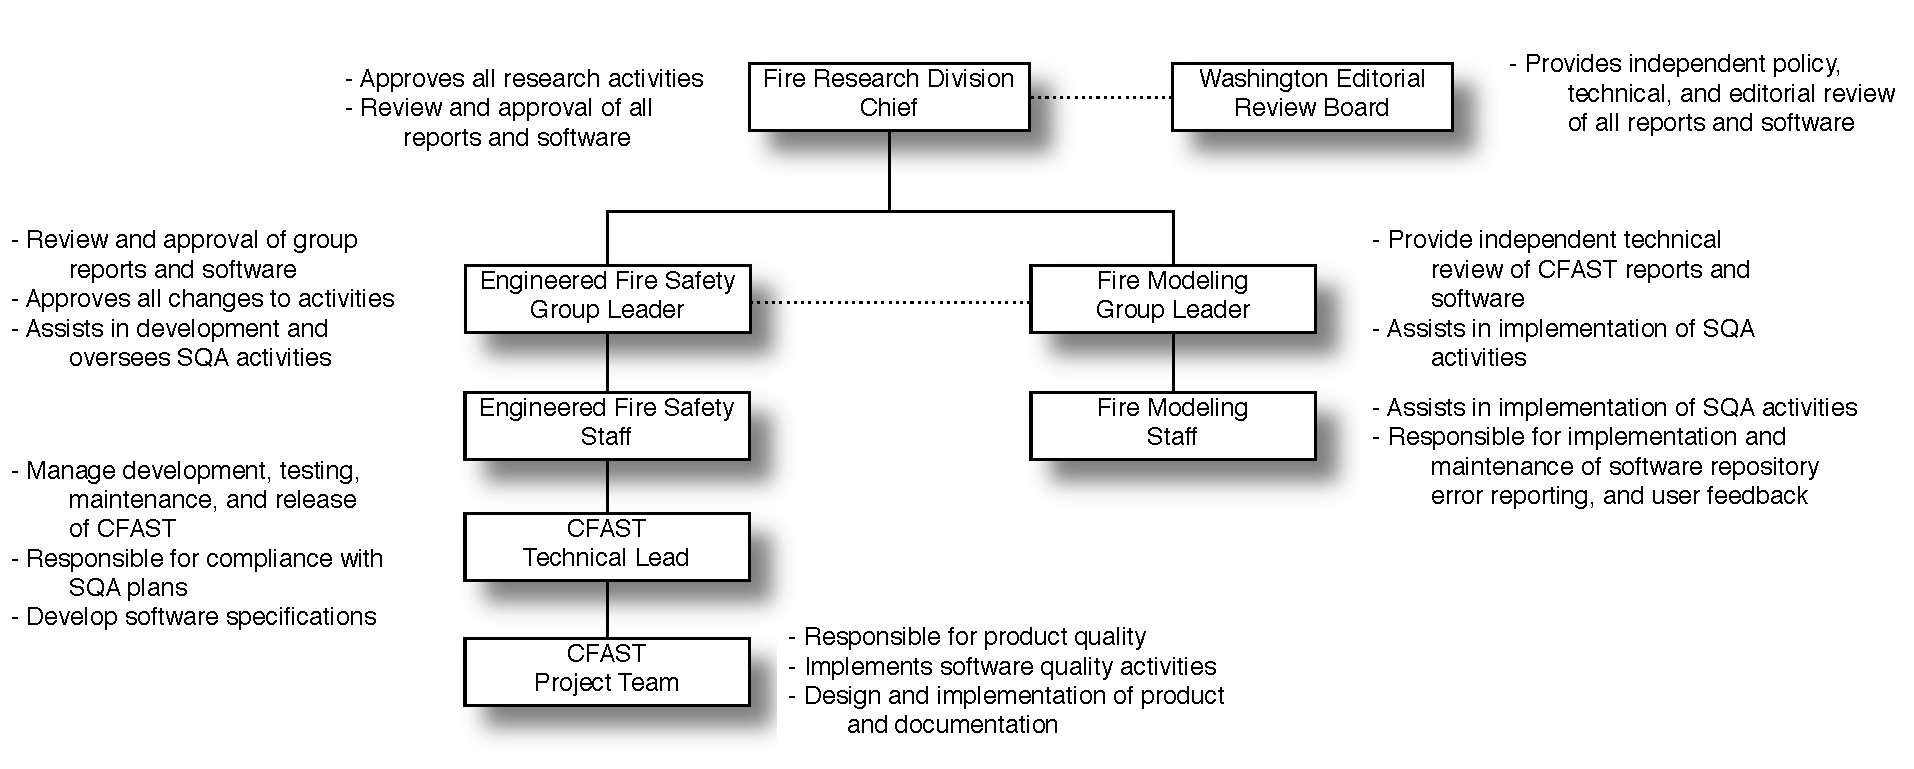
\includegraphics[width=6.5in]{FIGURES/OrgChart.pdf}\\
\end{center}
\caption{CFAST SQA Organization Structure.}
 \label{figOrgChart}
\end{figure}

Review and approval of software and documentation is part of the standard review process for any report or other product developed by NIST. A minimum of five reviews are required prior to release of reports or software, including two independent technical peer reviews, two technical and management reviews at the technical workgroup and division level, and a policy review at the NIST-wide level.  This review is documented and recorded on the NIST standard form NIST 114 along with official approval notification provided to the primary author of the product.

CFAST is distributed exclusively through a NIST website dedicated to the CFAST model (http://cfast.nist.gov).  Content of the website is the responsibility of the CFAST project leader and the BFRL webmaster. Additions and changes to the website are made only with the approval of the CFAST project leader after any required NIST reviews.

\section{SQA Documentation}

The released version of CFAST is documented by three primary publications, the Technical Reference Guide\cite{CFAST_Tech_Guide_6}, the User�s Guide \cite{CFAST_Users_Guide_6}, and this Software and Model Evaluation Guide. The documents apply to the newest version of the model available on the NIST website. The Technical Reference Guide describes the underlying physical principles, provides a review of model verification and validation efforts by NIST and others, and describes the limitations of the model.  The User's Guide describes how to use the model, includes a detailed description of the model inputs and outputs, and provides a process to ensure the correct installation of the model. There are also documents archived on the website that are applicable to older versions of both the model and user interface.

During development of new or corrected features for the model, the following documents are developed:

\begin{itemize}
\item {\em Software Requirements and Design Specifications:}  This is an internal memorandum that documents the intended function of a new or enhanced feature, describes its implementation in sufficient detail to allow an independent review of the feature, and identifies any new or existing testing and validation required prior to acceptance of the feature in a release version of the model.  This document forms the basis for necessary changes to the technical reference guide and user�s guide for the model once the new feature is ready for general release. As defined in IEEE 730-2002 \cite{IEEE:730}, this document includes the software requirements specification, software design description, and software verification and validation plan. The level of detail in this document depends on the complexity of the change to the model. 

\item {\em Software Validation and Testing Results:}  This is an internal memorandum that demonstrates the use of the new feature through appropriate test cases and describes validation and verification tests performed to ensure the new feature is implemented properly without unexpected changes in other features. This document forms the basis for the model verification and validation documentation included as part of this Software and Experimental Validation guide. As defined in IEEE 730-2002 \cite{IEEE:730}, this document includes the software verification and validation report. The level of detail in this document depends on the complexity of the change to the model.
\end{itemize}

Both of these documents are reviewed internally to NIST by group staff not directly involved with model development. In addition, the NIST review process documents the review and approval of released versions of the model as described above.

Source code for released versions of the model is maintained with version control software that allows tracking of specific changes to the model from version to version.   Each version of the model released includes a unique version number that identifies the major and minor version numbers of the release as well as the date of release. Differences with prior versions are documented and provided as part of the release and on the CFAST website so that users can ascertain what effect these changes will have on prior calculations.

\section{Standards, Practices, Conventions, and Metrics}

Prior to final implementation of a new feature or change, a review of the proposed modification is conducted by a developer who is not involved in the modification.  This review includes review and concurrence of the software requirements and design specification as well as more detailed review of code changes as the complexity of the modification requires. Review and acceptance of the software requirements and design specification by interested project sponsors or users may be included as appropriate. Name and date of approval and/or review is noted electronically in the document.

Review of the testing and validation report is also conducted by a developer who is not involved in the modification prior to proposed model release. Any significant changes in model output (typically a change greater than 1 \% of a given output) should be explained based on changes to the code as a result of a new feature.  Name and date of approval and/or review is noted electronically in the document.

\section{Software Reviews}

Software reviews are outlined as part of the standard practices described above.  The standard NIST review process includes review of software and documentation prior to any report or product release by NIST.

\section{Model Testing}

Individual testing of model algorithms are made by the developers during any revision of the model. Often, this testing forms the basis for any new standard test cases included with future model releases. System release testing of the model prior to release includes the following:

\begin{itemize}
\item Examination of results of test cases specific to any model modifications made as appropriate.  Comparison with analytic solutions to simplified problems is desirable when available.

\item Examination of results of standard test cases included with the release version of the model. Any changes in the output from prior versions is explained (and documented in the software testing and validation results report) by modifications made to the model.

\item For major new releases of the model, a complete suite of test cases should be compared to those from previous versions of the model.  At a minimum this includes the set of validation exercises described in NUREG 1824 \cite{NRCNUREG1824}, but may include additional example cases or validation exercises as appropriate.
\end{itemize}

\section{Problem Reporting and Resolution}

NIST maintains an e-mail address specifically for inquiries and problem reporting for the CFAST model (cfast@nist.gov).  These e-mails are directed to the CFAST project leader for response and resolution as appropriate.  Inquiries and responses are catalogued and retained by the project leader.

NIST has developed an automated reporting and resolution tracking website for use with the CFAST model to facilitate tracking and cataloging of inquires, problems, and model enhancements / revisions. This is included as part of the CFAST website at http://cfast.nist.gov

\section{Tools, Techniques, and Methodologies}

NIST will use an automated comparison tool (under development) to compare CFAST predictions between different versions of the model and with experimental data to simplify testing and validation for the CFAST model.

\section{Media Control}

Release versions of the CFAST model are available exclusively on the CFAST specific website maintained by the Building and Fire Research Laboratory (BFRL) at NIST. This website is included in NIST�s automated backup and recovery system for computer systems organization wide.

Development versions of the model are maintained by the CFAST project leader.  All software and documents are included in NIST�s automated backup and recovery system for computer systems organization wide.

Both of these computer systems are available only to specified personnel, including the CFAST project leader and BFRL webmaster.

\section{Supplier Control}

CFAST is entirely a product of BFRL / NIST and as such does not include any commercial software libraries. The differential equation solver used by CFAST, DASSL, is a publicly available software package.  Full source code for the solver as used by CFAST is maintained under version control with the rest of the model code.

BFRL currently uses Microsoft Visual Studio 2005 and Intel Visual Fortran 10.1 for development\footnote{Certain commercial entities, equipment, or materials may be identified in this document 
in order to describe an experimental procedure or concept adequately. Such identification 
is not intended to imply recommendation or endorsement by the National Institute of 
Standards and Technology, nor is it intended to imply that the entities, materials, or 
equipment are necessarily the best available for the purpose.}.  Prior to any change to a different development system, a full test suite of test cases must be compared to verify consistent operation of the model and model results.

\section{Records Collection, Maintenance, and Retention}

All software, documentation, and SQA documents are retained by the CFAST project leader, typically in electronic form. Software and documentation is also maintained and archived on the NIST CFAST website as part of the version control software for the model. 

BFRL management approval is required prior to destruction of old or out-of-date records. Records are typically maintained for a minimum of 25 years.

\section{Training}

No specific training is identified for use of this SQAP.  Details of training requirements for use of the model included in the CFAST user�s guide is applicable to developers of the model as well.

{\section{Risk Management}

The primary risk management tool for software developed and released by NIST is the official NIST review process for software, documents, and other products of NIST. Official approval is required prior to release of the model for general use.



\chapter{Software Structure and Verification}

The mathematical and numerical robustness of a deterministic computer model depends upon
three issues: the code must be transparent so that it can be understood and modified by visual
inspection; it must be possible to check and verify the coding implementation (perhaps with automated tools); and there must be a
method for checking the correctness of the solution, at least for asymptotic (steady state)
solutions (numerical stability and agreement with known solutions).

The terms {\em verification} and {\em validation} are often used interchangeably to mean the process of checking the
accuracy of a numerical model. For many, this entails comparing model predictions with experimental measurements. However,
there is now a fairly broad-based consensus that comparing model and experiment is largely what is considered {\em validation}. So what is
{\em verification}? ASTM~E~1355~\cite{ASTM:E1355}, ``Standard Guide for
Evaluating the Predictive Capability of Deterministic Fire Models,'' defines verification as
\begin{quote}
The process of determining that the implementation of a calculation method accurately
represents the developer's conceptual description of the calculation method and the solution to the calculation method.
\end{quote}
and it defines validation as
\begin{quote}
The process of determining the degree to which a calculation method is an accurate representation of the real world
from the perspective of the intended uses of the calculation method.
\end{quote}
Simply put, verification is a check of the math; validation is a check of the physics. If the model predictions closely match
the results of experiments, using whatever metric is appropriate, it is assumed by most that the model suitably describes, via
its mathematical equations, what is happening. It is also assumed that the solution of these equations must be correct. So why do
we need to perform model verification? Why not just skip to validation and be done with it? The reason is that rarely do model and
measurement agree so well in all applications that anyone would just accept its results unquestionably. Because there is
inevitably differences between model and experiment, we need to know if these differences are due to limitations or errors in
the numerical solution, or the physical sub-models, or both.

Whereas model validation consists mainly of comparing predictions with measurements, as documented later in this guide, 
model verification consists of a much broader range of activities, from checking the computer program
itself to comparing calculations to analytical (exact) solutions to understanding the impact on model outputs from a range of different model inputs.

In order to understand the meaning model verification, it is also  necessary to understand the
means by which the numerical routines are structured. In this chapter, details of the
implementation of the model are presented, including the tests used to assess the numerical
aspects of the model. These include:

\begin{itemize}
\item the structure of the model, including the major routines implementing the various
physical phenomena included in the model,
\item the organization of data initialization and data input used by the model,
\item the structure of data used to formulate the differential equations solved by the model,
\item a summary of the main control routines in the model that are used to control all input and
output, initialize the model and solve the appropriate differential equation set for the
problem to be solved,
\item the means by which the computer code is checked for consistency and correctness,
\item analysis of the numerical implementation for stability and error propagation, and
\item comparison of the results of the system model with simple analytical or numerical
solutions.
\item a series of reference test cases used to evaluate the impact of model changes to the full range of model outputs.
\end{itemize}

\section{Structure of the Numerical Routines}

A methodology which is critical to verification of the model is the schema used to incorporate
physical phenomena. This is the subroutine structure discussed below. The method for
incorporating new phenomena and ensuring the correctness of the code was adopted as part of
the consolidation of CCFM and FAST. This consolidation occurred in 1990 and has resulted in a
more transparent, transportable and verifiable numerical model. This transparency is crucial to a
verifiable and robust numerical implementation of the predictive model as discussed in the
sections on code checking and numerical analysis.

The model can be split into distinct parts. There are routines for reading data, calculating results
and reporting the results to a file or printer. The major routines for performing these functions
are identified in figure \ref{figCFASTStructure}. These physical interface routines link the CFAST model to the actual routines which calculate quantities such as mass or energy flow at one particular point in time for a given environment.

\begin{figure}[\figoptions{b}]
\begin{center}
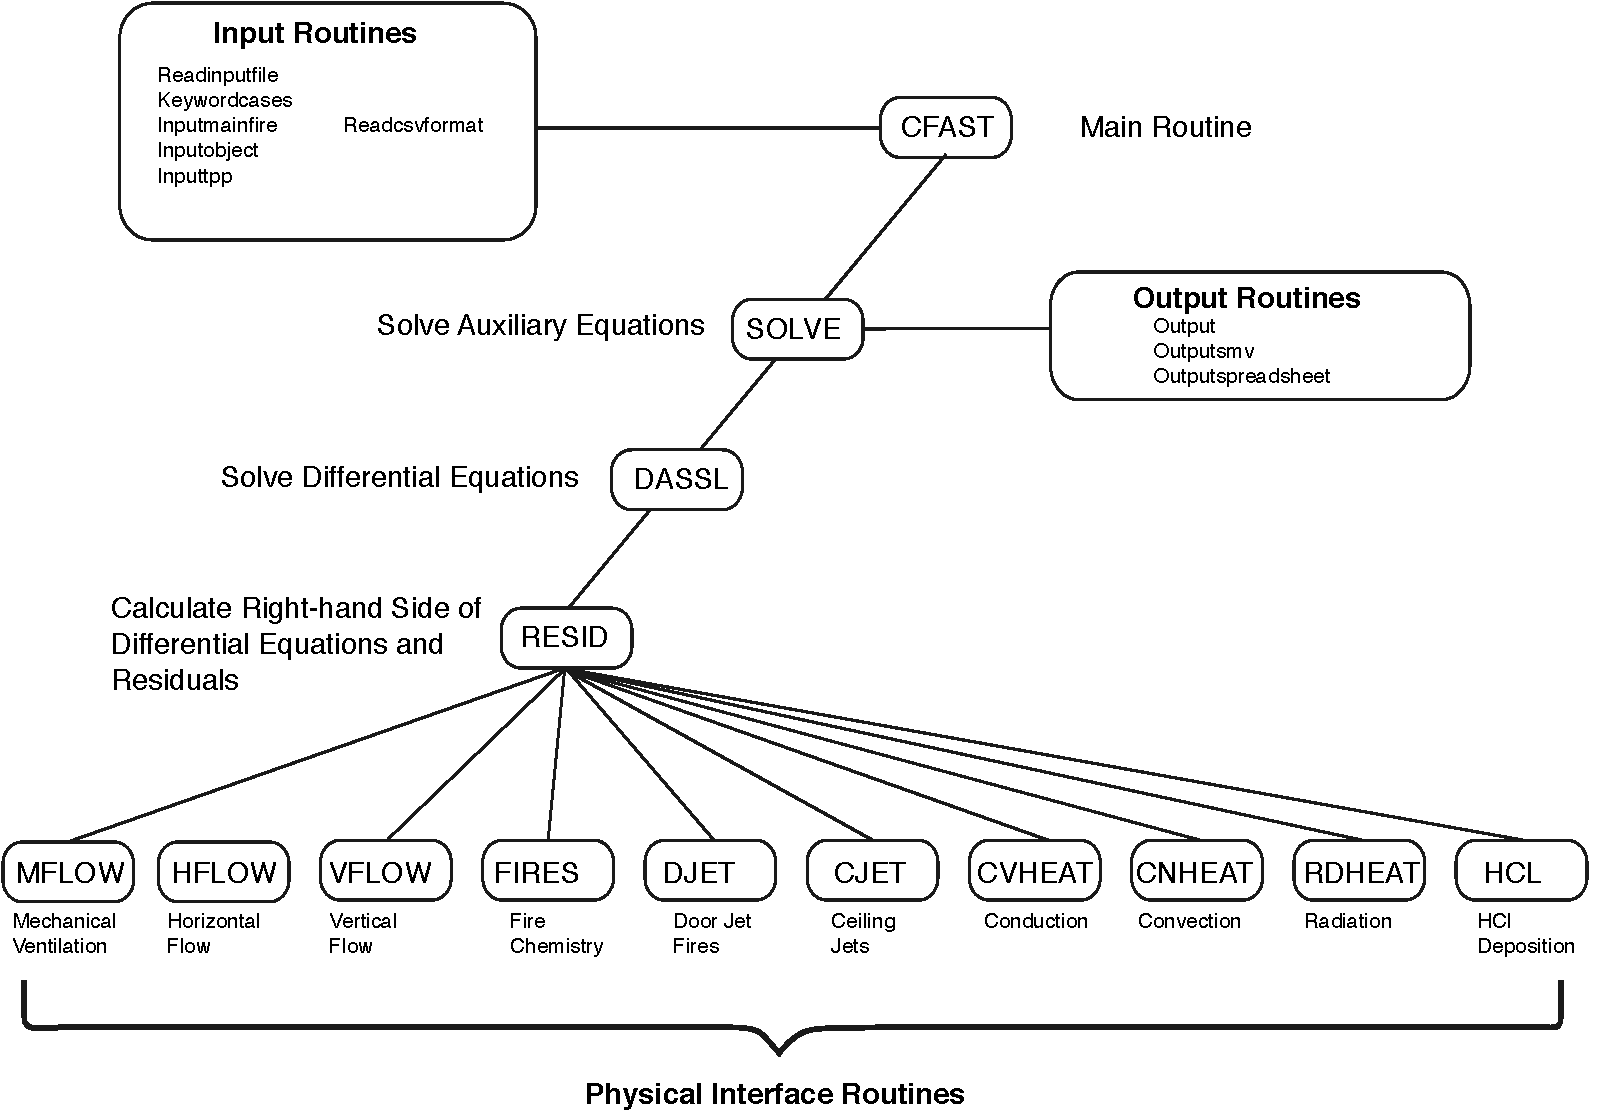
\includegraphics[width=4.4444in]{FIGURES/Structure}\\
\end{center}
\caption[Subroutine structure for the CFAST model]{Subroutine structure for the CFAST model showing major routines and calling structure.}
 \label{figCFASTStructure}
\end{figure}

The routines SOLVE, RESID and DASSL are the key to understanding how the physical
equations are solved. SOLVE is the control program that oversees the general solution of the
problem. It invokes the differential equation solver DASSL \cite{DASSL} which in turn calls RESID to
solve the transport equations. Given a solution at time t, what is the solution at time t plus a
small increment of time, $\dt$? The differential equations are of the form

\begin{eqnarray}
   \frac{{dy}}{{dx}} &=& f(y,t) \label{eqdiffeqform}  \\
    y(t_0 ) &=& y_0 \nonumber
\end{eqnarray}

where $y$ is a vector representing pressure, layer height, mass and such, and $f$ is a vector function that represents changes in these values with respect to time. The term $y_0$ is an initial condition at
the initial time $t_0$. The time increment is determined dynamically by the program to ensure convergence of the solution at $t + \Delta t$. The subroutine RESID computes the right hand side of eq \ref{eqdiffeqform} and returns a set of residuals of that calculation to be compared to the values expected by DASSL. DASSL then checks for convergence. Once DASSL reaches an error limit (defined as convergence of the equations) for the solution at $t + \Delta t$, SOLVE then advances the solution of species concentration, wall temperature profiles, and mechanical ventilation for the same time interval.
Note that there are several distinct time scales that are involved in the solution of this type of
problem. The fastest will be chemical kinetics. In CFAST, chemical reactions are assume to be instantaneous so we ignore the impact of chemical kinetics.  The next larger time scale is that associated with the flow field. These are the equations which are cast into the form of ordinary differential equations. Then there is the time scale for mechanical ventilation, and finally, heat conduction through objects.

Chemical kinetic times are typically on the order of milliseconds. The transport time scale are
on the order of 0.1 s. The mechanical ventilation and conduction time scales are typically
several seconds, or even longer. The time step is dynamically adjusted to a value appropriate for
the solution of the currently defined equation set. In addition to allowing a more correct solution
to the pressure equation, very large time steps are possible if the problem being solved
approaches steady-state.

\section{Numerical Tests}

CFAST is designed to use 64-bit precision for real number calculations to minimize the effects of numerical error.

The differential and algebraic equation solver (called DASSL) has been tested for a variety of differential equations and is widely used and accepted \cite{DASSL}.  The radiation and conduction routines have also been tested against known solutions for asymptotic results \cite{Forney_radiation}.

Coupling between the physical algorithms of the model and the differential equation solver also works to ensure numerical accuracy by dynamically adjusting the time step used by the model to advance the solutions of the equation set. Solution tolerances are set to require solution of the model equations within one part in $10{^6}$. This ensures that the error attributable to numerical solution is far less than that associated with the model assumptions.

\section{Code Checking}
Two standard programs have been used to check the CFAST model structure and language.  Specifically, FLINT and LINT have been applied to the entire model to verify the correctness of the interface, undefined or incorrectly defined (or used) variables and constants, and completeness of loops and threads.

The CFAST code has also been checked by compiling and running the model on a variety of computer platforms.  Because FORTRAN and C are implemented differently for various computers, this represents both a numerical check as well as a syntactic check.  CFAST has been compiled for Sun (Solaris), SGI (Irix), Microsoft Windows-based PCs (Lahey, Digital, and Intel FORTRAN), and Concurrent computer platforms.  Within the precision afforded by the various hardware implementations, the model outputs are identical on the different platforms. \footnote{Typically an error limit of one part in $10^6$ which is the limit set for the differential equation solver in the solution of the CFAST equations}

The CFAST Technical Reference Guide \cite{CFAST_Tech_Guide_6} contains a detailed description of the CFAST subroutine structure and interactions between the subroutines.

\section{Simple Analytical Comparisons}

Certain CFAST sub-models address phenomena that have analytical solutions, for example, one dimensional heat conduction through a solid or pressure increase in a sealed or slightly leaky compartment as a result of a fire or fan.  The developers of CFAST use analytical solutions to test sub-models to verify the correctness of the coding of the model as part of the development. This section provides an overview of the verification testing conducted with each change of the model to verify the basic underlying principles of the model, the mass and energy balances.

For most of the examples presented in this chapter, the same basic geometry is used, a single 5 m x 5 m x 5m compartment.  Depending on the exact simulation, additional details will be added to verify individual model results.  To begin, the simplest example is simply a compartment set at uniform ambient conditions with no ventilation, fires, or additional modeled features.  With no added mass or energy to the system, conditions are expected to remain at the initial ambient. Figure \ref{fig:Ambient_Conditions_Test} shows the simulated conditions for this simple test.

\begin{figure}
\begin{tabular*}{\textwidth}{l@{\extracolsep{\fill}}r}
\includegraphics[width=3.0in]{FIGURES/Verification/Ambient_Temperature} &
\includegraphics[width=3.0in]{FIGURES/Verification/Ambient_Pressure}
\end{tabular*}
\caption{Ambient conditions for test case with no fire, no vents, and non-conducting surfaces. Initial conditions set to 20 \degc. CFAST verification file Base.in.} \label{fig:Ambient_Conditions_Test}
\end{figure}

As a simple test of the energy balance,raising the external temperature of the base case compartment from an initial condition of 20~\degc to 25~\degc allows the temperature to equilibrate to the exterior. With conducting compartment surfaecs, the interior compartment temeprature is expected to equilibrate to the exterior. From the ideal gas law, the pressure rise can be calculated as

\begin{eqnarray}
   \frac{P_i V_i}{N_i R T_i} &=&  \frac{P_f V_f}{N_f R T_f} \label{eq:Temperature_Equilibrium}  \\
   P_f &=& T_f\frac{P_i}{T_i}  \nonumber \\
  P_f &=& 298.15 \frac{101300}{293.15} \nonumber \\
  &=& 103027.78 \text{\ Pa} \nonumber
\end{eqnarray}

or a pressure rise of 1727.78, matching the output from CFAST.  Figure \ref{fig:Temperature_Equilibrium} shows the simulated conditions for this test.

\begin{figure}
\begin{tabular*}{\textwidth}{l@{\extracolsep{\fill}}r}
\includegraphics[width=3.0in]{FIGURES/Verification/Temperature_Equilibrium_Test} &
\includegraphics[width=3.0in]{FIGURES/Verification/Pressure_Change_Temperature_Equilibrium_Test}
\end{tabular*}
\caption{Ambient conditions for test case with no fire and Gypsum board surfaces, with intenral initial temperature of 20~\degc and external initial temperature of 25~\degc. CFAST verification file basic\_tempequilib.in.} \label{fig:Temperature_Equilibrium}
\end{figure}

The same test can be repeated with all surfaces turned off.  With the absence of conductive surfaces, compartment conditions are not expected to change. Figure \ref{fig:Different_Ambients_Nonconducting}  shows the simulated conditions for the test case.

\begin{figure}
\begin{tabular*}{\textwidth}{l@{\extracolsep{\fill}}r}
\includegraphics[width=3.0in]{FIGURES/Verification/Temperature_Equilibrium_Walls_Off} &
\includegraphics[width=3.0in]{FIGURES/Verification/Pressure_Change_Temperature_Equilibrium_Test_With_Walls_Off}
\end{tabular*}
\caption{Ambient conditions for test case with no ventilation and non-conducting surfaces.  Exterior conditions set to 25 \degc.  CFAST verification file basic\_tempequilib\_wallsoff.in.} 
\label{fig:Different_Ambients_Nonconducting}
\end{figure}

The compartment surfaces are then turned back on, returning to the original base case.  With exterior conditions set to 25 \degc and an open window present, conditions are expected to equilibrate to those of the exterior. For this example, the open window allows the pressure to equlibrate as well. Figure \ref{fig:Temperature_Equilibrium_With_Window} shows the simulated conditions for the test case.

\begin{figure}
\begin{tabular*}{\textwidth}{l@{\extracolsep{\fill}}r}
\includegraphics[width=3.0in]{FIGURES/Verification/Temperature_Equilibrium_Test_With_Window} &
\includegraphics[width=3.0in]{FIGURES/Verification/Pressure_Change_Temperature_Equilibrium_Test_With_Window}
\end{tabular*}
\caption{Ambient conditions for test case with no ventilation and non-conducting surfaces.  Exterior conditions set to 25 \degc.  CFAST verification file basic\_tempequilib\_window.in.} 
\label{fig:Temperature_Equilibrium_With_Window}
\end{figure}

To test both the mass and energy balance, consider the base case with the addition of a fixed amount of ambient air (injected through a mechanical vent.  The vent is set to deliver 0.1 m$^3$/s into the compartment for 10 s. After this, the vent is closed.  Over the 10 s period, an additional 1 m$^3$ of air at ambient temperature is added.  Since CFAST, by default, closes vent over a 1 s time period, an additional 0.05 m$^3$ is also added. With a compartment volume of 125~m$^3$ at 20 \degc, the initial mass of air is 150.5 kg or 5.195 moles. With the added mass, the final mass of air in the compartment is 151.7 kg or 5.239 moles. From the CFAST output, the final temperature of the compartment rises slightly due to the pressure increase to 20.98 \degc. From the ideal gas law, the expected pressure rise can be calculated as

\begin{eqnarray}
   \frac{P_i V_i}{N_i R T_i} &=&  \frac{P_f V_f}{N_f R T_f} \label{eq:Added_Mass}  \\
   P_f &=& \frac{P_i N_f  T_f}{N_i T_i}  \nonumber \\
  P_f &=& \frac{101300 \cdot 5.239 \cdot 294.13}{5.195 \cdot 293.15} \nonumber \\
  &=& 102491.3 \text{\ Pa} \nonumber
\end{eqnarray}

or a pressure rise of 1191.3 Pa, matching the calculated CFAST output to within 0.002~\%. Figure \ref{fig:Added_Mass_Test} shows the simulated conditions for this test.

\begin{figure}
\begin{tabular*}{\textwidth}{l@{\extracolsep{\fill}}r}
\includegraphics[width=3.0in]{FIGURES/Verification/Ambient_Temperature_Added_Mass} &
\includegraphics[width=3.0in]{FIGURES/Verification/Ambient_Pressure_Added_Mass}
\end{tabular*}
\caption{Ambient conditions for test case with no fire and non-conducting surfaces, with a mechanical ventilation system injecting 0.1~m$^3$/s of air into the compartment for 10 s. CFAST verification file Added\_Mass.in.} \label{fig:Added_Mass_Test}
\end{figure}

A model examining heat added to a system can be demonstrated with a test case containing a constant 100 kW fire.  With non-conducting surface and no ventilation, the heat and mass released by the fire (and added to the compartment) can be determined.  Here we use a single zone simulation to simplfy the calculations (CFAST simply assumes the entire volume is taken up by the upper layer).  Densities are obtained using the calculated temperature. The energy and mass added to the system can be calculated as

\begin{eqnarray}
M_0 &=& V \cdot \rho_{ambient} \nonumber \\
 &=& 150 \cdot 1.195 \nonumber \\
 &=& 149.39 \text{\ kg} \nonumber \\
M &=& M_0 + \dm_f \cdot t \\
E_0 &=& M_0 \cdot c_v \cdot T_{ambient} \nonumber \\
 &=& 149.39 \cdot 1012/1.4 \cdot 293.15 \nonumber \\
 &=& 31.65  \text{\ MJ} \nonumber \\
E &=& E_0 + Q_f \cdot t + \dm_f \cdot c_v \cdot T
\end{eqnarray}
where $M_0$ is the initial mass of air in the compartment, $V$ is the compartment volume, $\rho_{ambient}$ is the air density at ambient conditions, $M$ is the mass of gases in the compartment at time $t$\, $\dm_f$ is the pyrolysis rate of the burning fuel, $E_0$ is the initial internal energy of the system, $c_v$ is the heat capacity of air at constant volume, $T_{ambient}$ is the temperature of the compartment at ambient conditions, $E$ is the internal energy of the system at time $t$, $Q_f$ is the convective heat release rate of the fire, and $T$ is the temperature of the compartment at time $t$.

Finally, the temperature of the compartment can be calculated from the definition of internal energy of the system

\begin{equation}
E = M \cdot c_v \cdot T \text{, or, rearranging, } T = \frac{E}{c_v \cdot M}
\end{equation} 

Figure \ref{fig:Analytical_Closed_Compartment} shows the comparison of the calculated and CFAST results for this test. The average difference between the calculations is approximately 0.01 \%, with the difference due to the way CFAST handles a single layer calculation while maintaining its default equation set that includes both a lower and upper layer.

\begin{figure}
\begin{center}
\includegraphics[width=3.0in]{FIGURES/Verification/Sealed_Compartment_Temperature}
\caption{Comparison of CFAST calculations and analytical solution for a 100 kW fire in a closed 5 m x 5 m x 5 m compartment.  CFAST verification file sealed\_test.in.}
\label{fig:Analytical_Closed_Compartment}
\end{center}
\end{figure}

\section{Simple Reference Cases}

In addition to the comparisons of test cases with analytical solutions discussed in the previous section, we have included a number of simple test cases intended to demonstrate the impact of individual model features.  While these are too complex to provide analytical solutions, many can be estimated with simpler engineering calculations.  Together, these form a set of simulations that can be routinely run to verify continued consistency of the calculation results as the model is further developed to insure unintended side-effects of modifications to the model are prevented.

For completeness, the first examples dupicate the simple examples in the previous section. As in the previous section,  most of the examples presented in this section share the same basic geometry, a single 5 m x 5 m x 5 m compartment. Unless otherwise detailed, the ‘base case’ has a single window centered on the front wall that is 2 m x 1 m and has 5/8 in Gypsum Board walls and ceiling. Depending on the exact simulation, additional details will be added to verify individual model results. 

\subsection{Ambient Conditions}

To begin, the simplest example is the base case compartment set at uniform ambient conditions with no ventilation, fires, or additional modeled features. With no added mass or energy to the system, conditions are expected to remain at the initial ambient. Figure \ref{fig:Ambient_Conditions_Reference} shows the simulated conditions for this simple test.

\begin{figure}
\begin{tabular*}{\textwidth}{l@{\extracolsep{\fill}}r}
\includegraphics[width=3.0in]{FIGURES/Verification/Ambient_Temperature} &
\includegraphics[width=3.0in]{FIGURES/Verification/Ambient_Pressure}
\end{tabular*}
\caption{Ambient conditions for test case with no fire, no vents, and non-conducting surfaces. Initial conditions set to 20 \degc. CFAST verification file Base.in.} \label{fig:Ambient_Conditions_Reference}
\end{figure}

With the exterior temperature still set to 25 \degc, the elevation is raised to 1500 m, approximately the average elevation of Idaho.  Since CFAST calculations are relative to the exterior ambient, conditions are expected to be identical to the previous examples and equilibrate to those of the exterior. Figure \ref{fig:Temperature_Equilibrium_Elevation} shows the simulated conditions for the test case.

\begin{figure}
\begin{tabular*}{\textwidth}{l@{\extracolsep{\fill}}r}
\includegraphics[width=3.0in]{FIGURES/Verification/Temperature_Equilibrium_Elevation_Change} &
\includegraphics[width=3.0in]{FIGURES/Verification/Pressure_Change_Temperature_Equilibrium_Test_Elevation}
\end{tabular*}
\caption{Ambient conditions for test case with no ventilation and non-conducting surfaces.  Exterior conditions set to 25 \degc and elevation to 1500 m.  CFAST verification file basic\_tempequilib\_window\_elevation.in.} 
\label{fig:Temperature_Equilibrium_Elevation}
\end{figure}

With the exterior temperature still set to 25 \degc, the compartment dimensions are altered to 10 m x 10 m x 5 m.  Conditions are predicted to equilibrate to those of the exterior more slowly than that of the base case model. Figure \ref{fig:Temperature_Equilibrium_Bigger} shows the simulated conditions for the test case.

\begin{figure}
\begin{tabular*}{\textwidth}{l@{\extracolsep{\fill}}r}
\includegraphics[width=3.0in]{FIGURES/Verification/Temperature_Equilibrium_Compartment_Dimension_Change} &
\includegraphics[width=3.0in]{FIGURES/Verification/Pressure_Change_Temperature_Equilibrium_Test_Compartment}
\end{tabular*}
\caption{Ambient conditions for test case with no ventilation and non-conducting surfaces.  Exterior conditions set to 25 \degc and compartment dimensions enlarged to 10 m x 10 m x 10 m..  CFAST verification file basic\_tempequilib\_window\_geometry.in.} 
\label{fig:Temperature_Equilibrium_Bigger}
\end{figure}

With the exterior temperature still set to 25 \degc, the wind is raised to 10 m/s.  Temperature conditions are expected to equilibrate to those of the exterior, while the pressure will remain at a constant pressure greater than zero due to wind pressure.  Figure \ref{fig:Temperature_Equilibrium_Wind_Speed} shows the simulated conditions for the test case.

\begin{figure}
\begin{tabular*}{\textwidth}{l@{\extracolsep{\fill}}r}
\includegraphics[width=3.0in]{FIGURES/Verification/Temperature_Equilibrium_Wind_Speed_Change} &
\includegraphics[width=3.0in]{FIGURES/Verification/Pressure_Change_Temperature_Equilibrium_Test_Wind}
\end{tabular*}
\caption{Ambient conditions for test case with no ventilation and non-conducting surfaces.  Exterior conditions set to 25 \degc and compartment dimensions enlarged to 10 m x 10 m x 10 m..  CFAST verification file basic\_tempequilib\_window\_geometry.in.} 
\label{fig:Temperature_Equilibrium_Wind_Speed}
\end{figure}

Returning to the base case input, the interior pressure is lowered from the default value of 101300 Pa down to 100000 Pa.  Conditions are expected to equilibrate to those of the exterior.  Figure \ref{fig:Pressure_Equilibrium} shows the simulated conditions for the test case.

\begin{figure}
\begin{tabular*}{\textwidth}{l@{\extracolsep{\fill}}r}
\includegraphics[width=3.0in]{FIGURES/Verification/Temperature_Change_Pressure_Equilibrium_Test_With_Window} &
\includegraphics[width=3.0in]{FIGURES/Verification/Pressure_Equilibrium_Ventilation}
\end{tabular*}
\caption{Ambient conditions for test case with ventilation and conducting surfaces. Interior pressure is initially set to 100000 Pa.  CFAST verification file basic\_pressure\_vent.in.} 
\label{fig:Pressure_Equilibrium}
\end{figure}

\subsection{Ventilation}

All ambient conditions are returned to the standard base case.  A mechanical vent is added to the test case with a flow rate of 0.1 m$^3$/s for 10 s. Figure \ref{fig:Mechanical_Vent_Cutoff} shows the pressure building in the compartment for the default fan cutoff pressure of 200 Pa to 300 Pa compared to a raised fan cutoff pressure of 2000 Pa.

\begin{figure}
\begin{center}
\includegraphics[width=3.0in]{FIGURES/Verification/Pressure_Dropoff_Test}
\caption{Model with mechanical vent and non-inhibited drop off pressure of 2000 Pa versus model with mechanical vent and interfering drop off pressure of 200 Pa..  CFAST verification files basic\_mechvent\_n.csv and basic\_mechvent\_dropoff\_n.csv.}
\label{fig:Mechanical_Vent_Cutoff}
\end{center}
\end{figure}

Two identical 5 m x 5 m x 5m compartments are stacked on each other.  A 1 m$^2$ mechanical vent is added on the front face of compartment one, the shared ceiling/floor between compartment one and two, and the rear wall of compartment two.  The flow rate is set to 0.1 m$^3$/s or 0.12 kg/s of air.  The mass flow through each of these vents is expected to the same because the flow rate in is constant and there is no change in temperature.   Figure \ref{fig:Mechanical_Flow_Two_Compartments} shows vent flows for all vents in the simulation.

\begin{figure}
\begin{center}
\includegraphics[width=3.0in]{FIGURES/Verification/Mass_Flow_Test_Mechanical_Vent}
\caption{Side-by-side base case compartments with mechanical vents added from outside to compartment one, compartment one to compartment two, and compartment two to outside.  CFAST verification file basic\_connection\_floorceiling\_mechvent.in.}
\label{fig:Mechanical_Flow_Two_Compartments}
\end{center}
\end{figure}

\subsection{Fire Characteristics}

A fire was added to the base case.  The fire is positioned at X=2.5 m, Y=2.5 m, Z= 0, with a methane fire at a maximum heat release rate of 1054 kW. All other fire inputs remain as the standard setting. Unless otherwise defined, the following reference cases contain this defined fire.

\begin{figure}
\begin{center}
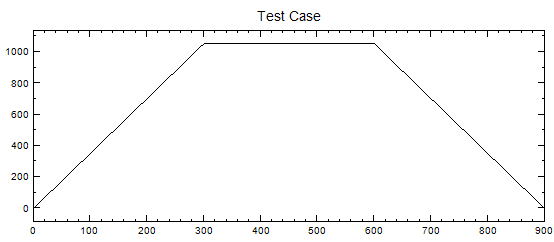
\includegraphics[width=5.772in]{FIGURES/Verification/Test_Case_HRR.png}
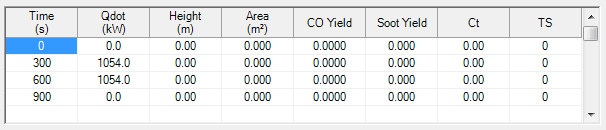
\includegraphics[width=5.772in]{FIGURES/Verification/Test_Case_HRR_Chart.png}
\caption{Simple defined fire for base case model with added fire.}
\label{fig:Base_Fire_Configuration}
\end{center}
\end{figure}

Figure \ref{fig:Fire_Base} shows compartment temperatures, layer height, and species concentrations for the base case with a 1054 kW fire.

\begin{figure}
\begin{tabular*}{\textwidth}{l@{\extracolsep{\fill}}r}
\includegraphics[width=3.0in]{FIGURES/Verification/Temperature_Fire_Base} &
\includegraphics[width=3.0in]{FIGURES/Verification/HGT_Fire_Base}
\end{tabular*}
\begin{center}
\includegraphics[width=3.0in]{FIGURES/Verification/Species_Production_Fire_Base}
\end{center}
\caption{Test case conditions for the base case model with a 1054 kW fire and no vent.  CFAST verification file fire.in.} 
\label{fig:Fire_Base}
\end{figure}

Returning to the base case with an added fire, the heat release rate curve was then altered to have the same area under the curve but a different shape.  The altered curve had a maximum heat release rate of 1333.3 kW and reached peak heat release rate at 450 s. The altered fire is shown in Figure \ref{fig:Altered_Fire_Configuration}. Figure \ref{fig:Fire_Alternate_HRR} shows the base fire and alternate fire.

\begin{figure}
\begin{center}
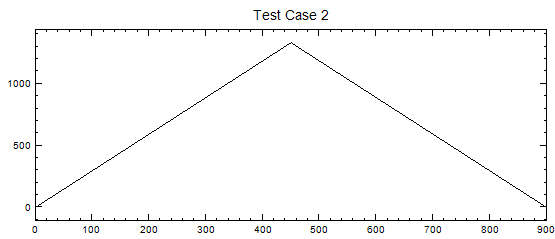
\includegraphics[width=5.772in]{FIGURES/Verification/Test_Case_Altered_HRR.png}
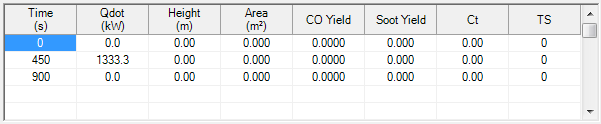
\includegraphics[width=5.772in]{FIGURES/Verification/Test_Case_Altered_HRR_Chart.png}
\caption{Alternate defined fire for base case model with added fire with the same total heat released as the base fire from Figure \ref{fig:Base_Fire_Configuration}.}
\label{fig:Altered_Fire_Configuration}
\end{center}
\end{figure}

\begin{figure}
\begin{tabular*}{\textwidth}{l@{\extracolsep{\fill}}r}
\includegraphics[width=3.0in]{FIGURES/Verification/Temperature_HRR_Area_Base} & \includegraphics[width=3.0in]{FIGURES/Verification/Temperature_HRR_Area_Change} \\
\includegraphics[width=3.0in]{FIGURES/Verification/HGT_HRR_Area_Base} & \includegraphics[width=3.0in]{FIGURES/Verification/HGT_HRR_Area_Change} \\
\includegraphics[width=3.0in]{FIGURES/Verification/Species_Production_HRR_Area_Base} & \includegraphics[width=3.0in]{FIGURES/Verification/Species_Production_HRR_Area_Change} 
\end{tabular*}
\caption{Test case conditions for the base case model with a trapezoidal 1054 kW fire and a single 1 m x 2 m window (left) and a triangular 1333 kW fire and a single 1 m x 2 m window. The same total heat is released in both fires.  CFAST verification file fire\_HRRarea2.in.} 
\label{fig:Fire_Alternate_HRR}
\end{figure}

The chemical composition of the fire can also be changed in CFAST.  Figure \ref{fig:fire_fuel_composition} shows the base fire configuration with a window with several different fual compositions for the fire.

\begin{figure}
\begin{center}
\includegraphics[width=3.0in]{FIGURES/Verification/Upper_Layer_Temperature_Materials} \\
\includegraphics[width=3.0in]{FIGURES/Verification/Lower_Layer_Temperature_Materials} \\
\includegraphics[width=3.0in]{FIGURES/Verification/HGT_Materials} 
\caption{Test case conditions for the base case model with a 1054 kW fire and a single 1 m x 2 m window with several different fuel compositions (methane, hexane, urethane, and wood) for the fire.  CFAST verification file fire\_fuels.in.} 
\label{fig:fire_fuel_composition}
\end{center}
\end{figure}

Returning to the base case with a window vent, the soot yield is changed to 0.5 kg/kg.  Figure \ref{fig:fire_soot_yield} shows the results.

\begin{figure}
\begin{center}
\begin{tabular*}{\textwidth}{l@{\extracolsep{\fill}}r}
\includegraphics[width=3.0in]{FIGURES/Verification/Species_Production_Soot_Yield_O2} & \includegraphics[width=3.0in]{FIGURES/Verification/Species_Production_Soot_Yield_CO2} \\
\includegraphics[width=3.0in]{FIGURES/Verification/Species_Production_Soot_Yield_H2O} & \includegraphics[width=3.0in]{FIGURES/Verification/Species_Production_Soot_Yield_OD}
\end{tabular*}
\caption{Test case conditions with the soot yield raised to 0.500, versus the base case model.  CFAST verification file fire\_sootyield.in.} 
\label{fig:fire_soot_yield}
\end{center}
\end{figure}

\subsection{Fires and Ventilation}

Figures \ref{fig:Fire_Window} to \ref{fig:Fire_Window_Compartment_Mechanical_Vent_Only} show a range of cases that vary the ventilation in the compartment, keeping the fire input constant.

\begin{figure}
\begin{tabular*}{\textwidth}{l@{\extracolsep{\fill}}r}
\includegraphics[width=3.0in]{FIGURES/Verification/Temperature_Fire_Base} & \includegraphics[width=3.0in]{FIGURES/Verification/Temperature_Window} \\
\includegraphics[width=3.0in]{FIGURES/Verification/HGT_Fire_Base} & \includegraphics[width=3.0in]{FIGURES/Verification/HGT_Window} \\
\includegraphics[width=3.0in]{FIGURES/Verification/Species_Production_Fire_Base} & \includegraphics[width=3.0in]{FIGURES/Verification/Species_Production_Window} 
\end{tabular*}
\caption{Test case conditions for the base case model with a 1054 kW fire and no vent (left) with the same model with a single 1 m x 2 m window (right).  CFAST verification file fire\_window.in.} 
\label{fig:Fire_Window}
\end{figure}

\begin{figure}
\begin{tabular*}{\textwidth}{l@{\extracolsep{\fill}}r}
\includegraphics[width=3.0in]{FIGURES/Verification/Temperature_Window} & \includegraphics[width=3.0in]{FIGURES/Verification/Temperature_Two_Windows} \\
\includegraphics[width=3.0in]{FIGURES/Verification/HGT_Window} & \includegraphics[width=3.0in]{FIGURES/Verification/HGT_Two_Windows} \\
\includegraphics[width=3.0in]{FIGURES/Verification/Species_Production_Window} & \includegraphics[width=3.0in]{FIGURES/Verification/Species_Production_Two_Windows} 
\end{tabular*}
\caption{Test case conditions for the base case model with a 1054 kW fire and a single 1 m x 2 m window (left) with the same model with a two 1 m x 2 m windows (right).  CFAST verification file fire\_window\_windowchange.in.} 
\label{fig:Fire_Two_Windows}
\end{figure}

\begin{figure}
\begin{tabular*}{\textwidth}{l@{\extracolsep{\fill}}r}
\includegraphics[width=3.0in]{FIGURES/Verification/Temperature_Window} & \includegraphics[width=3.0in]{FIGURES/Verification/Temperature_Ceiling_Vent} \\
\includegraphics[width=3.0in]{FIGURES/Verification/HGT_Window} & \includegraphics[width=3.0in]{FIGURES/Verification/HGT_Ceiling_Vent} \\
\includegraphics[width=3.0in]{FIGURES/Verification/Species_Production_Window} & \includegraphics[width=3.0in]{FIGURES/Verification/Species_Production_Ceiling_Vent} 
\end{tabular*}
\caption{Test case conditions for the base case model with a 1054 kW fire and a single 1 m x 2 m window (left) with the same model with 2 m$^2$ ceiling vent replacing the window vent (right).  CFAST verification file fire\_ceiling.in.} 
\label{fig:Fire_Window_Compartment_Vertical_Vent}
\end{figure}

\begin{figure}
\begin{tabular*}{\textwidth}{l@{\extracolsep{\fill}}r}
\includegraphics[width=3.0in]{FIGURES/Verification/Temperature_Window} & \includegraphics[width=3.0in]{FIGURES/Verification/Temperature_Mechanical_Only_Vent} \\
\includegraphics[width=3.0in]{FIGURES/Verification/HGT_Window} & \includegraphics[width=3.0in]{FIGURES/Verification/HGT_Mechanical_Only_Vent} \\
\includegraphics[width=3.0in]{FIGURES/Verification/Species_Production_Window} & \includegraphics[width=3.0in]{FIGURES/Verification/Species_Production_Mechanical_Only_Vent} 
\end{tabular*}
\caption{Test case conditions for the base case model with a 1054 kW fire and a single 1 m x 2 m window (left) with the same model with a mechanical vent replacing the window vent (right).  CFAST verification file fire\_ceiling.in.} 
\label{fig:Fire_Window_Compartment_Mechanical_Vent_Only}
\end{figure}

\subsection{Compartment Geometry}

Figure \ref{fig:Fire_Window_Compartment_Aspect_Ratio} shows the results of a  simulation where the aspect ratio of the compartment is changed from the base model of 5 m x 5 m to one 10 m x 2.5 m.  Ceiling height and other details are the same as the base case.

\begin{figure}
\begin{tabular*}{\textwidth}{l@{\extracolsep{\fill}}r}
\includegraphics[width=3.0in]{FIGURES/Verification/Temperature_Window} & \includegraphics[width=3.0in]{FIGURES/Verification/Temperature_Window_Aspect_Ratio} \\
\includegraphics[width=3.0in]{FIGURES/Verification/HGT_Window} & \includegraphics[width=3.0in]{FIGURES/Verification/HGT_Window_Aspect_Ratio} \\
\includegraphics[width=3.0in]{FIGURES/Verification/Species_Production_Window} & \includegraphics[width=3.0in]{FIGURES/Verification/Species_Production_Window_Aspect_Ratio} 
\end{tabular*}
\caption{Test case conditions for the base case model with a 1054 kW fire and a single 1 m x 2 m window (left) with the same model with the compartment aspect ratio changed to 10 m x 2.5 m x 5 m (right).  CFAST verification file fire\_window\_aspect\_ratio.in.} 
\label{fig:Fire_Window_Compartment_Aspect_Ratio}
\end{figure}

Figure \ref{fig:Fire_Window_Compartment_Geometry_Increase} shows the results of a simulation where the size of the compartment  is increased from the base model of 5 m x 5 m to one 10 m x 10 m.  Ceiling height and other details are the same as the base case.

\begin{figure}
\begin{tabular*}{\textwidth}{l@{\extracolsep{\fill}}r}
\includegraphics[width=3.0in]{FIGURES/Verification/Temperature_Window} & \includegraphics[width=3.0in]{FIGURES/Verification/Temperature_Compartment_Geometry_Increase} \\
\includegraphics[width=3.0in]{FIGURES/Verification/HGT_Window} & \includegraphics[width=3.0in]{FIGURES/Verification/HGT_Compartment_Geometry_Increase} \\
\includegraphics[width=3.0in]{FIGURES/Verification/Species_Production_Window} & \includegraphics[width=3.0in]{FIGURES/Verification/Species_Production_Compartment_Geometry_Increase} 
\end{tabular*}
\caption{Test case conditions for the base case model with a 1054 kW fire and a single 1 m x 2 m window (left) with the same model with the compartment size increased to 10 m x 10 m x 5 m (right).  CFAST verification file fire\_window\_windowchange.in.} 
\label{fig:Fire_Window_Compartment_Geometry_Increase}
\end{figure}

\subsection{Sprinklers}

The following plots compare the base case model to an array of test cases that vary the sprinkler feature of CFAST.  The following test cases include a graph depicting the sensor activation time.  When these graphs rise from zero to one, this indicates the time that the sprinkler was activated.  The sprinkler was added at X=2.5 m, Y=2.5 m, and Z=4.95 m.  Figure \ref{fig:fire_sprinkler_base} shows the base case fire with a single 1 m by 2 m window with and without a sprinkler.  Sprinkler was defined with an operating temperature of 57 \degc (135 \degf), an RTI of 100~$\sqrt{\text{m~s}}$, and a spray density of 7 x 10$^{-5}$ m/s. Figure \ref{fig:fire_sprinkler_density} shows results with the spray density doubled, Figure \ref{fig:fire_sprinkler_RTI} shows results with the RTI cut in half, and Figure \ref{fig:fire_sprinkler_HRR_doubled} shows results with the peak heat release rate of the fire doubled. 

\begin{figure}
\begin{tabular*}{\textwidth}{l@{\extracolsep{\fill}}r}
\includegraphics[width=3.0in]{FIGURES/Verification/Temperature_Sprinkler} & \includegraphics[width=3.0in]{FIGURES/Verification/HGT_Sprinkler} \\
\includegraphics[width=3.0in]{FIGURES/Verification/Sensor_Activation_Time_Sprinkler} & \includegraphics[width=3.0in]{FIGURES/Verification/Species_Production_Sprinkler} 
\end{tabular*}
\caption{Test case conditions for the base case model with a 1054 kW fire and a single 1 m x 2 m window (left) with the same model with a sprinkler added (right).  CFAST verification file fire\_sprinkler.in.} 
\label{fig:fire_sprinkler_base}
\end{figure}

\begin{figure}
\begin{tabular*}{\textwidth}{l@{\extracolsep{\fill}}r}
\includegraphics[width=3.0in]{FIGURES/Verification/Temperature_Sprinkler_Density_Doubled} & \includegraphics[width=3.0in]{FIGURES/Verification/HGT_Sprinkler_Density_Doubled} \\
\includegraphics[width=3.0in]{FIGURES/Verification/Sensor_Activation_Time_Sprinkler_Density_Doubled} & \includegraphics[width=3.0in]{FIGURES/Verification/Species_Production_Sprinkler_Density_Doubled} 
\end{tabular*}
\caption{Test case conditions for the base case model with a 1054 kW fire, a single 1 m x 2 m window, and a sprinkler (left), with the same model with the sprinkler spray density doubled (right).  CFAST verification file fire\_sprinkler\_density.in.}
\label{fig:fire_sprinkler_density}
\end{figure}

\begin{figure}
\begin{tabular*}{\textwidth}{l@{\extracolsep{\fill}}r}
\includegraphics[width=3.0in]{FIGURES/Verification/Temperature_Half_Sprinkler_RTI} & \includegraphics[width=3.0in]{FIGURES/Verification/HGT_Half_Sprinkler_RTI} \\
\includegraphics[width=3.0in]{FIGURES/Verification/Sensor_Activation_Time_Half_Sprinkler_RTI} & \includegraphics[width=3.0in]{FIGURES/Verification/Species_Production_Half_Sprinkler_RTI} 
\end{tabular*}
\caption{Test case conditions for the base case model with a 1054 kW fire, a single 1 m x 2 m window, and a sprinkler (left), with the same model with the sprinkler RTI reduced by 50~\% (right).  CFAST verification file fire\_sprinkler\_RTI.in.}
\label{fig:fire_sprinkler_RTI}
\end{figure}

\begin{figure}
\begin{tabular*}{\textwidth}{l@{\extracolsep{\fill}}r}
\includegraphics[width=3.0in]{FIGURES/Verification/Temperature_Sprinkler_and_HRR_Doubled} & \includegraphics[width=3.0in]{FIGURES/Verification/HGT_Sprinkler_and_HRR_Doubled} \\
\includegraphics[width=3.0in]{FIGURES/Verification/Sensor_Activation_Time_Sprinkler_and_HRR_Doubled} & \includegraphics[width=3.0in]{FIGURES/Verification/Species_Production_Sprinkler_and_HRR_Doubled} 
\end{tabular*}
\caption{Test case conditions for the base case model with a 1054 kW fire, a single 1 m x 2 m window, and a sprinkler (left), with the same model with the peak heat release rate of the fire doubled (right).  CFAST verification file fire\_sprinkler\_HRRdoubled.in.}
\label{fig:fire_sprinkler_HRR_doubled}
\end{figure}

\section{Complex Examples}

In addition to the numerous validation experiements included in this guide, organizations have developed a number of detailed example cases with different versions of CFAST.  This section includes a selection of these cases run with the current version of CFAST.

\subsection{NRC Fire Modeling Application Guide Examples}

The U.S. Nuclear Regulatory Commission provides guide to users of fire model for nuclear power plant applications in NUREG-1934 \cite{NRCNUREG1934}.  This section presents the outputs (using the current version of CFAST) for the four of these example applications that included analysis using CFAST. Table\ref{tab:NUREG_1934_Tests} shows the four examples included in this section.

\begin{table}[h!]
\caption[Summary of NRC example scenarios from NUREG-1934]{Summary of NRC example scenarios from NUREG-1934  \cite{NRCNUREG1934} run using CFAST}
\begin{center}
\begin{tabular*}{\textwidth}{|c|@{\extracolsep{\fill}}L{5.0in}|}
\hline
Example & Scenario Description \\ \hline \hline
A & Determination of the time to main control room abandonment given a low voltage panel fire. \\ \hline
B & Determination of the potential for a switchgear panel fire to damage cables above the fire and adjacent to the fire. \\ \hline
D & Determination of the potential for a motor control center panel fire to damage cables via the hot gas layer in an irregularly-shaped enclosure \\ \hline
E & Determination of the potential for a transient trash fire to damage cables in a stack of horizontal cable trays located directly above the fire \\ \hline
\end{tabular*}
\end{center}
\label{tab:NUREG_1934_Tests}
\end{table}

\begin{figure}
\begin{tabular*}{\textwidth}{l@{\extracolsep{\fill}}r}
\includegraphics[width=3.0in]{FIGURES/Verification/ULT_NRC_Test_1} & \includegraphics[width=3.0in]{FIGURES/Verification/HGT_NRC_Test_1} \\
\includegraphics[width=3.0in]{FIGURES/Verification/Heat_Flux_NRC_Test_1} & \includegraphics[width=3.0in]{FIGURES/Verification/OD_NRC_Test_1} 
\end{tabular*}
\caption{Test case conditions for the NRC main control room fire scenario.  CFAST verification file Cabinet\_fire\_in\_MCR.in.}
\label{fig:NRC_Scenario_A}
\end{figure}

\begin{figure}
\begin{tabular*}{\textwidth}{l@{\extracolsep{\fill}}r}
\includegraphics[width=3.0in]{FIGURES/Verification/Temperature_Cable_A_NRC_Test_2} & \\
\includegraphics[width=3.0in]{FIGURES/Verification/Temperature_Cabinet_A_NRC_Test_2} & \includegraphics[width=3.0in]{FIGURES/Verification/Heat_Flux_Cabinet_A_NRC_Test_2} 
\end{tabular*}
\caption{Test case conditions for the NRC cabinet fire in swithgear room scenario.  CFAST verification file Cabinet\_fire\_in\_switchgear.in.}
\label{fig:NRC_Scenario_B}
\end{figure}

\begin{figure}
\begin{tabular*}{\textwidth}{l@{\extracolsep{\fill}}r}
\includegraphics[width=3.0in]{FIGURES/Verification/Temperature_Cabinet_NRC_Test_4} & \includegraphics[width=3.0in]{FIGURES/Verification/Heat_Flux_Cabinet_NRC_Test_4} \\
\includegraphics[width=3.0in]{FIGURES/Verification/Temperature_Cables_NRC_Test_4} & \includegraphics[width=3.0in]{FIGURES/Verification/Heat_Flux_Cables_NRC_Test_4} 
\end{tabular*}
\caption{Test case conditions for the NRC motor control center fire in switchgear room scenario.  CFAST verification file MCC\_in\_switchgear.in.}
\label{fig:NRC_Scenario_D}
\end{figure}

\begin{figure}
\begin{tabular*}{\textwidth}{l@{\extracolsep{\fill}}r}
\includegraphics[width=3.0in]{FIGURES/Verification/ULT_NRC_Test_5} & \includegraphics[width=3.0in]{FIGURES/Verification/Flame_HGT_NRC_Test_5} \\
\includegraphics[width=3.0in]{FIGURES/Verification/Temperature_Cables_NRC_Test_5} & \includegraphics[width=3.0in]{FIGURES/Verification/Heat_Flux_Cables_NRC_Test_5} 
\end{tabular*}
\caption{Test case conditions for the NRC transient fire in cable spreading room scenario.  CFAST verification file Trash\_fire\_in\_cable\_spreading\_room.in.}
\label{fig:NRC_Scenario_E}
\end{figure}

\newpage

\subsection{DOE Example Cases}
\chapter{Survey of Past Validation Work}

CFAST has been subjected to extensive validation studies by NIST and others.  There are two ways of comparing predictive capability with actual events. The first is simply graphing the time series curves of model results with measured values of variables such as temperature. Another approach is to consider the time to critical conditions such as flashover. Making such direct comparisons between theory and experiment provides a sense of whether predictions are reasonable. This chapter provides a review of CFAST validation efforts by NIST and others to better understand the quality of the predictions by the model.

Some of the work has been  performed at NIST, some by its grantees and some by engineering firms using the model.  Because each organization has its  own reasons for  validating the model, the  referenced papers and reports do not follow any particular guidelines. Some of the works only provide  a qualitative assessment  of the model,  concluding that the  model  agreement with  a  particular  experiment  is ``good''  or ``reasonable.'' Sometimes, the conclusion is that the model works well in certain cases, not as well in others. These studies are included in the survey because the references  are useful to other model users who may have a similar application  and are interested in qualitative assessment. It is important to note  that some of the papers point out flaws in early releases of CFAST that have been corrected or improved in more recent  releases. Some of  the issues raised, however,  are still subjects of  active research. Continued updates for CFAST  are greatly influenced  by   the  feedback   provided  by  users,   often  through publication of validation efforts.


\section{Comparisons with Full-Scale Tests Conducted Specifically for the Chosen Evaluation}

Several studies have been conducted specifically to validate the use of CFAST in building performance design. Dembsey   \cite{Valid:Dempsey} used CFAST version 3.1 to predict the ceiling jet temperatures, surface heat fluxes and heat transfer coefficients for twenty compartment fire experiments in a compartment that is similar in size, geometry, and construction to the standard fire test compartment specified in the Uniform Building Code \cite{UBC}\footnote{The 1997 Uniform Building Code has been superceded by the International Building Code, 2003 Edition, International Code Council, Country Club Hills, Illinois.}. Results from 330 kW, 630 kW, and 980 kW fires were used. In general, CFAST made predictions which were higher than the experimental results. In these cases, the temperature prediction is typically 20 \% to 30 \% higher than measured values. Much of this can be attributed to not knowing the species production (soot) and relative absorption of radiation by the gas layers which highlights the importance of scenario specification. This is the most common cause of  �over prediction� of temperature by CFAST. A secondary source of discrepancy is correcting for radiation from thermocouple beads. The authors provide for this correction, but the corrections cited are not as large as has been reported in other fire experiments \cite{Valid:Pitts}.

He et al. \cite{Valid:He} describe a series of full-scale fire experiments that were designed to investigate the validity of two zone models including CFAST version 3.1. The experiments, involving steady state burning rates and a number of ventilation conditions, were conducted in a four-story building. Temperature, pressure, flow velocity, smoke density and species concentrations were measured in various parts of the building. The stack effect and its influence on temperature distribution in a stair shaft were observed. Comparisons were then made between the experimental results and the model predictions. Early in the fire there is a few percent difference\footnote{Unless otherwise noted, percent differences are defined as (model-experiment)/experiment x100.} between the predictions and measurements; beyond 10 min, there are significant variations. Both the experiment and the model are internally consistent; that is, higher flow leads to a higher interface height (figure 13 in the paper). Once again, the difference is about 25 \%. The authors discuss the effect of fuel composition and correction for radiation from thermocouple beads but did not draw firm conclusions based on their measurements of fuel products.

A series of experimental results for flaming fires, obtained using realistic fires in a prototype apartment building were performed by Luo et al. \cite{Valid:Luo}. Fuel configurations in the fire test included a horizontal plain polyurethane slab, mock-up chair (polyurethane slabs plus a cotton linen cover), and a commercial chair. CFAST version 3.1 typically over-predicted upper layer temperatures by 10 \% to 50 \% depending on the test conditions and measurement location in that test. The predicted and experimental time dependent upper layer temperatures were similar in shape. The time to obtain peak upper layer temperatures was typically predicted to within 15 \% of the experimental measurements. The authors concluded that CFAST was conservative in terms of life safety calculations.

In order to optimize fire service training facilities, the best use of resources is imperative. The work reported by Poole et al. \cite{Valid:Poole} represents one aspect of a cooperative project between the city of Kitchener Fire Department (Canada) and the University of Waterloo aimed at developing design criteria for the construction of a fire fighter training facility. One particular criterion is that realistic training with respect to temperature, heat release and stratification be provided in such a facility. The purpose of this paper was to compare existing analytical heat release and upper and lower gas temperature rise correlations and models with data from actual structures which were instrumented and burned in collaboration with the Kitchener Fire Department. According to the authors, the CFAST model was used `successfully' to predict these conditions and will be used in future design of such facilities.

A report by Bailey et al. \cite{Valid:Bailey_Shadwell} compares predictions by CFAST version 3.1 to data from real scale fire tests conducted onboard ex-USS SHADWELL, the {Navy's} R\&D damage control platform. The phenomenon of particular interest in this validation series was the conduction of heat in the vertical direction through compartment ceilings and floors. As part of this work, Bailey et al. \cite{Valid:Bailey_Vertical_Heat} compared CFAST temperature predictions on the unexposed walls of large metal boxes, driven by steady state fires. This tested the model�s prediction of radiation and conduction in both the vertical and horizontal directions. Indirectly it quantifies the quality of the conduction/convection/radiation models. The model and experiment compared well within measurement error bounds of each. The comparison was particularly good for measurements in the fire compartment as well as for the compartment and deck directly above it, with predictions typically agreeing with experiments within measurement uncertainty. The model under-predicted the temperatures of the compartments and decks not directly adjacent to the fire compartment early in the tests. Most of the error arose due to uncertainty in modeling the details of the experiment. The size of the vent openings between decks and to the outside must be included, but these were not always known. Cracks formed in the deck between the fire compartment and the compartment above due to the intense fire in the room of origin, but a time dependent record was not kept. The total size of the openings to the outside of warped doors in both compartments was not recorded. As can be seen in figures 7 and 8 of reference \cite{Valid:Bailey_Shadwell}, the steady state predictions are identical (within error bounds of the experiment and prediction). The largest error is after ignition (uncertainty in the initial fire) and during development of the cracks between the compartments. While this does not affect the agreement in the room of origin, it does lead to an error of about 30 \% in the adjacent compartment.

\section{Comparisons with Previously Published Test Data}

A number of researchers have studied the level of agreement between computer fire models and
real-scale fires. These comparisons fall into two broad categories: fire reconstruction and
comparison with laboratory experiments. Both categories provide a level of verification for the
models used. Fire reconstruction, although often more qualitative, provides a higher degree of
confidence for the user when the models successfully simulate real-life conditions. Comparisons
with laboratory experiments, however, can yield detailed comparisons that can point out
weaknesses in the individual phenomena included in the models.

Deal \cite{Valid:Deal} reviewed four computer fire models (CCFM \cite{Models:CCFM}, FIRST \cite{Models:FIRST}, FPETOOL \cite{Models:FPETool} and FAST \cite{Models:FAST}) version 18.5 (the immediate predecessor to CFAST) to ascertain the relative performance of the models in simulating fire experiments in a small room (about 12 m$^3$ in volume) in which the vent and fuel effects were varied. Peak fire size in the experiments ranged up to 800 kW. According to the author, all the models simulated the experimental conditions including temperature, species generation, and vent flows `quite satisfactorily.' With a variety of conditions, including narrow and normal vent widths, plastic and wood fuels, and flashover and sub-flashover fire temperatures, competence of the models at these room geometries was `demonstrated.'

\subsection{Fire Plumes}

Davis compared predictions by CFAST version 5 (and other models) for high ceiling spaces \cite{Valid:Davis_Plumes}. In this paper, the predictive capability of two algorithms designed to calculate plume centerline temperature and maximum ceiling jet temperature in the presence of a hot upper layer were compared to measurements from experiments and to predictions using CFAST�s ceiling jet algorithm. The experiments included ceiling heights of 0.58 m to 22 m and heat release rates of 0.62 kW to 33 MW. When compared to the experimental results CFAST�s ceiling jet algorithm tended to over-predict the upper layer temperature by 20 \%. With proper adjustment for radiation effects in the thermocouple measurements, some of this difference disappears. The effect of entrainment of the upper layer gases was identified for improvement.

\subsection{Multiple Compartments}
\label{secMultipleCompartments}

Jones and Peacock \cite{Valid:Jones} presented a limited set of comparisons between the FAST model (version 18.5) and a multi-room fire test. The experiment involved a constant fire of about 100 kW in a three-compartment configuration of about 100 m$^3$. They observed that the model predicted an upper layer temperature that was too high by about 20 \% with satisfactory prediction of the layer interface position. These observations were made before the work of Pitts et al. \cite{Valid:Pitts} showed that the thermocouple measurements need to be corrected for radiation effects. Convective heating and plume entrainment were seen to limit the accuracy of the predictions. A comparison of predicted and measured pressures in the rooms showed within 20 \%. Since pressure is the driving force for flow between compartments, this agreement was seen as important.

Levine and Nelson \cite{Valid:Levine} used a combination of full-scale fire testing and modeling to simulate a fire in a residence. The 1987 fire in a first-floor kitchen resulted in the deaths of three persons in an upstairs bedroom, one with a reported blood carboxyhemoglobin content of 91 \%. Considerable physical evidence remained. The fire was successfully simulated at full scale in a fully-instrumented seven-room two-story test structure. The data collected during the test have been used to test the predictive abilities of two multiroom computer fire models: FAST and HARVARD VI. A coherent ceiling layer flow occurred during the full-scale test and quickly carried high concentrations of carbon monoxide to remote compartments. Such flow is not directly accounted for in either computer code. However, both codes predicted the carbon monoxide buildup in the room most remote from the fire. Prediction of the pre-flashover temperature rise was also `good' according to the authors. Prediction of temperatures after flashover that occurred in the room of fire origin was seen as `less good.' Other predictions of conditions throughout the seven test rooms varied from `good approximations' to `significant deviations' from test data. Some of these deviations are believed to be due to combustion chemistry in the not upper layer not considered in detail in either of the two models.

\subsection{Large Compartments}

Duong \cite{Valid:Duong} studied the predictions of several computer fire models (CCFM, FAST, FIRST, and BRI \cite{Models:BRI}), comparing the models with one another and with large fires (4 MW to 36 MW) in an aircraft hanger (60 000 m$^3$). For the 4 MW fire size, he concluded that all the models are `reasonably accurate.' At 36 MW, however, `none of the models did well.' Limitations of the heat conduction and plume entrainment algorithms were thought to account for some of the inaccuracies.

\subsection{Prediction of Flashover}

A chaotic event that can be predicted by mathematical modeling is that of flashover. Flashover is
the common term used for the transition a fire makes from a few objects pyrolyzing to full room
involvement. It is of interest to the fire service because of the danger to fire fighters and to
building designers because of life safety and the attendant impact on occupants. Several papers
have looked at the capability of CFAST to predict the conditions under which flashover can
occur.

Chow \cite{Valid:Chow_Flashover} concluded that FAST correctly predicted the onset of flashover if the appropriate criteria were used. The criteria were gas temperature near the ceiling, heat flux at the floor level and flames coming out of the openings. This analysis was based on a series of compartment
fires.

A paper by Luo et al. \cite{Valid:Luo_Flashover} presents a comparison of the results from CFAST version 3 against a comprehensive set of data obtained from one flashover fire experiment. The experimental results were obtained from a full-scale prototype apartment building under flashover conditions. Three polyurethane mattresses were used as fuel. It was found that the predicted temperatures from the CFAST fire model agreed well with the experimental results in most areas, once radiation corrections are applied to the thermocouple data.

Collier \cite{Valid:Collier} makes an attempt to quantify the fire hazards associated with a typical New
Zealand dwelling with a series of experiments. These tests, done in a three-bedroom dwelling,
included both non-flashover and flashover fires. The predictions by CFAST version 2 were seen by the author as consistent with the experiments within the uncertainty of each.

Post-flashover fires in shipboard spaces have a pronounced effects on adjacent spaces due to
highly conductive boundaries. CFAST (version 3.1) predictions for the gas temperature and the
cold wall temperature were compared with shipboard fires \cite{Valid:White}. The comparisons between the model and experimental data show `conservative predictions' According to the authors. The authors attribute this to an overestimation of the average hot wall temperature and an underestimation of external convective losses due to wind effects.

Finally, a comparison of CFAST with a number of simple correlations was used by
Peacock and Babrauskas \cite{Valid:Peacock_Flashover_1,Valid:Peacock_Flashover_2} to simulate a range of geometries and fire conditions to predict the development of the fire up to the point of flashover. The simulations represent a range of compartment sizes and ceiling heights. Both the correlations and CFAST predictions were seen to provide a lower bound to observed occurrence of flashover. For very small or very large compartment openings, the differences between the correlations, experimental data, and CFAST predictions was more pronounced.

The important test of all these prediction methods is in the comparison of the predictions with
actual fire observations. Figure \ref{figValidFlashover} (reference \cite{Valid:Peacock_Flashover_2}) presents estimates of the energy required to achieve flashover for a range of room and vent sizes. This figure is an extension of the earlier work of Babrauskas  \cite{Valid:Babrauskas_Flashover} and includes additional experimental measurements from a variety of sources, most notably the work of Deal and Beyler \cite{Valid:DealandBeyler}. For a number of the experimental observations, values are included that were not 
explicitly identi�ed as being a minimum value at flashover. In addition, figure \ref{figValidFlashover} includes predictions from the CFAST model (version 5).

\begin{figure}[\figoptions{b}]
\begin{center}
\includegraphics[width=5.0000in]{FIGURES/flashover.pdf}\\
\end{center}
\caption{Comparison of correlations, CFAST predictions, and experimental data for the prediction of flashover in a compartment fire.}
 \label{figValidFlashover}
\end{figure}

As with some of the experimental data defining flashover as an upper layer temperature reaching
600 $^{\circ}$C, many experimental measures were reported as peak values rather than minimum values necessary to achieve flashover. Thus, ideally all the predictions should provide a lower bound
for the experimental data. Indeed, this is consistent with the graph � the vast majority of the
experimental observations lie above the correlations and model predictions. For a considerable
range in the ratio \asqh, the correlations of Babrauskas \cite{Valid:Babrauskas_Flashover} Thomas \cite{Thomas:1981fk}, and the MQH correlation of McCaffrey et al. \cite{McCaffrey:1981uq} provide similar estimates of the minimum energy required to produce flashover. The estimates of H\"{a}gglund \cite{Hagglund:1980} yields somewhat higher estimates for values of \asqh  \, greater than 20 m$^{-1/2}$.

The results from the CFAST model for this single compartment scenario provide similar results
to the experiments and the correlations for most of the range of \asqh. For small values of \asqh, the CFAST values rise somewhat above the values from the correlations. These small values of \asqh \, result from either very small compartments (small $A_T$) or very large openings (large \asqh), both of which stretch the limits of the assumptions inherent in the model. For very small compartments, radiation from the fire to the compartment surfaces becomes more important, enhancing the conductive heat losses through the walls. However, the basic two-zone assumption may break down as the room becomes very small. For very large openings, the calculation of vent flow via an orifice flow coefficient approach is likely inaccurate. Indeed, for such openings, this limitation has been observed experimentally \cite{Valid:Babrauskas_Flashover}. The estimates are close to the range of uncertainty shown by the correlations which also diverge at very small values of \asqh.

Perhaps most significant in these comparisons is that all the simple correlations provide estimates similar to the CFAST model and all the models are consistent with a wide range of experimental data. For this simple scenario, little is gained with the use of the more complex models. For more complicated scenarios, the comparison may not be as simple.

\section {Comparison with Documented Fire Experience}

There are numerous cases of CFAST being used to adjudicate legal disputes. Since these are discussed in courts of law, there is a great deal of scrutiny of the modeling, assumptions, and results. Most of these simulations and comparisons are not available in the public literature. A few of the cases which are available are discussed below. The metric for how good the model performed is its ability to reproduce the time-line as observed by witnesses and the death of occupants or the destruction of property as was used in evidence in legal proceedings.

As mentioned in section \ref{secMultipleCompartments}, Levine and Nelson describe the use of FAST for understanding the deaths of two adults in a residence in Sharon, Pennsylvania in 1987 \cite{Valid:Levine}. The paper compared the evidence of the actual fire, a full scale mockup done at NIST and the results from FAST (version 18) \cite{Jones:1985} and Harvard VI \cite{Rockett:1985}. The most notable shortcoming of the models was the lower than actual temperatures in the bedrooms, caused by loss of heat through the fire barriers. This led to the improvement in CFAST in the mid-90s to couple compartments together so that both horizontal and vertical heat transfer can occur to adjacent compartments.

Bukowski used CFAST version 3.1 to analyze a fire in New York City \cite{Bukowski:1996} in 1994 which resulted in the death of three fire fighters. The CFAST model was able to reproduce the observed conditions and supported the theory as to how the fire began and the cause of death of the three fire fighters.

Chow describes the use and comparison of CFAST simulations with a 1996 high rise building fire in Hong Kong \cite{Chow:1996}. CFAST simulations were performed to help understand the probable fire environment under different conditions. Three simulations were performed to study the consequences of a fire starting in the lift shaft. Smoke flow in the simulations qualitatively matched those observed during the incident.

In the early morning hours of March 25,1990 a tragic fire took the lives of 87 persons at a neighborhood club in the Bronx, New York \cite{Bukowski:1992}. The New York City Fire Department requested the assistance of the NIST Center for Fire Research (CFR) in understanding the factors which contributed to this high death toll and to develop a strategy that might reduce the risk of a similar occurrence in the many similar clubs operating in the city. The simulation showed the potential for development of untenable conditions within the club and particularly in the single exit stairway.

\section{Comparison with Experiments Which Cover Special Situations}

There are several sets of comparisons used in the development of the model or specific
applications beyond those discussed more generally above.

\subsection{Nuclear Facilities}

Floyd validated CFAST version 3.1 by comparing the modeling results with measurements from fire tests at
the Heiss-Dampf Reaktor (HDR) facility \cite{Floyd:2002}. The structure was originally the containment
building for a nuclear power reactor in Germany. The cylindrical structure was 20 m in diameter
and 50 m in height topped by a hemispherical dome 10 m in radius. The building was divided
into eight levels. The total volume of the building was approximately 11 000 m$^3$. From 1984 to
1991, four fire test series were performed within the HDR facility. The T51 test series consisted
of 11 propane gas tests and three wood crib tests. To avoid permanent damage to the test facility,
a special set of test rooms were constructed, consisting of a fire room with a narrow door, a long
corridor wrapping around the reactor vessel shield wall, and a curtained area centered beneath a
maintenance hatch. The fire room walls were lined with fire brick. The doorway and corridor
walls had the same construction as the test chamber. Six gas burners were mounted in the fire
room. The fuel source was propane gas mixed with 10 \% air fed at a constant rate to one of the
six burners.

In general, the comparison between CFAST and the HDR results was seen as `good' by the author, with two exceptions. The first is the over estimate of the temperature of the upper layer, typically within about 15 \% of the experimental measurements. This is common and generally results from the using too low a value for the production of soot, water (hydrogen) and carbon monoxide. The other exception consists of predictions in spaces where the zone model concept breaks down, for example in the stairways between levels. In this case, CFAST has to treat the space either in the filling mode (two layer approximation) or as a fully mixed zone (using the SHAFT option). Neither is quite correct, and in order to understand the condition in such spaces in detail (beyond the transfer of mass and energy), a more detailed CFD model must be used, for example, FDS \cite{FDS_Tech_Guide_5}.

The U.S. Nuclear Regulatory Commission performed an extensive verification and validation of several fire models commonly used in nuclear power plant applications \cite{NRCNUREG1824}.  These models included simple spreadsheet calculations, zone models (including CFAST \cite{NRCNUREG1824_CFAST}), and CFD models. The results of this study are presented in the form of relative differences between fire model predictions and experimental data for fire modeling attributes such as temperature or heat flux that are important to NPP fire modeling applications.  These relative differences are affected by the capabilities of the models, the availability of accurate applicable experimental data, and the experimental uncertainty of these data. Evaluation of the two-zone models showed that the models simulated the experimental results within experimental uncertainty  for many of the parameters of interest. The reason for this may be that the relatively simple experimental configurations selected for this study conform well to the simple two-layer assumption that is the basis of these models. 

While the relative differences sometimes show agreement for many parameters, they also show both under-prediction and over-prediction in some circumstances, most notably when conditions vary within a compartment or detailed local conditions are important to accurate prediction (for example, plume temperature or heat flux near to the fire source). The results and comparisons included the the NRC study are included in this report for the current version of CFAST.

\subsection{Small Scale Testing}

As an implementation of the zone model concept, CFAST is applicable to a wide range of scenarios. One end of this spectrum are small compartments, one to two meters on a side. Several research efforts have looked at small scale validation. There are three papers by Chow \cite{Lui:2003,Chow:1995,Chow:1992} which examine this issue. The first is the use of an electric heater with adjustable thermal power output was to verify temperature predictions by CFAST version 3.1. The second was closed chamber fires studied by burning four types of organic liquids, namely ethanol, N-heptane, and kerosene. The burning behavior of the liquids was observed, and the hot gas temperature measured. These behaviors along with the transient variations of the temperature were then compared with those predicted by the CFAST model. Finally, in another series of experiments, three zone models, one of which was CFAST, were evaluated experimentally using a small fire chamber. Once again, liquid fires were chosen for having better control on the mass loss rate. The results on the development of smoke layer and the hot gas temperature predicted by the three models were compared with those measured experimentally. According to Chow, `fairly good agreement' was found if the input parameters were carefully chosen.

\subsection{Unusual Geometry and Specific Algorithms}

A zone model is inherently a volume calculation. There is an assumption in the derivation of the equations that gas layers are strongly stratified. This allows for the usual interpretation that a volume can then be thought of as a rectangular parallelepiped, which allows the developers to express the volume in terms of a floor area and height of a compartment, saying simply that the height times the floor area is the volume. However, there are other geometries which can be adequately described by zone models. Tunnels, ships, and attics are the most common areas of application which fall outside of the usual scope.

\subsubsection{Railway and Vehicle Tunnels}

Altinakar et al. \cite{Altinakar:1997} used a \emph{modified version} of CFAST for predicting fire development and smoke propagation in vehicle or railroad tunnels. The two major modifications made to the model dealt with mixing between the upper and lower layers and friction losses along the tunnel. The model was tested by simulating several full-scale tests carried out at memorial Tunnel Ventilation Test Program in West Virginia, and the Offeneg Tunnel in Switzerland. His article compares simulated values of temperature, opacity and similar sensible quantities with measured values and discusses the limits of the applicability of zone models for simulating fire and smoke propagation in vehicle and railroad tunnels. 

Peacock et al. \cite{Peacock:2004} compared times to untenable conditions determined from tests in a
passenger rail car with those predicted by CFAST for the same car geometry and fire scenarios.
For a range of fire sizes and growth rates, they found agreement that averaged approximately
13 \%.

\subsubsection{Non-Uniform Compartments}

In January 1996, the U.S. Navy began testing how the CFAST model would perform when tasked with predicting shipboard fires. These conditions include mass transport through vertical vents (representing hatches and scuttles), energy transport via conduction through decks, improvement to the radiation transport sub-model, and geometry peculiar to combat ships. The purpose of this study was to identify CFAST limitations and develop methods for circumnavigating these problems \cite{Hoover:2001}. A retired ship representing the forward half of a {USS} Los Angeles class submarine was used during this test. Compartments in combat ships are not square in floor area, nor do they have parallel sides.

Application of CFAST to these scenarios required a direct integration of compartment cross-sectional area as a function of height to correctly interpret the layer interface position and provide correct predictions for flow through doors and windows (vertical vents). This required user specification of the area as a function of height (ROOMA and ROOMH inputs) to provide a description for the model to use. For most applications of CFAST, the effort required for the input outweighs any additional precision in the calculated results gained by use of the ROOMA and ROOMH inputs in the model.

\subsubsection{Long Corridors}

Prior to development of the corridor flow model, the implementation of flow in compartments assumed that smoke traveled instantly from one side of a compartment to another. The work of Bailey et al. \cite{Bailey:2002} provided the basis for the corridor flow model in CFAST. According to the author, it shows `good agreement' for the delay time calculated using CFAST version 5 and measured flow along high aspect ratio passageways.

\subsubsection{Mechanical Ventilation}

There have been two papers which have looked at the effectiveness of the mechanical ventilation system. The first considered a fire chamber of length 4.0 m, width 3.0 m and height 2.8 m with adjustable ventilation rates \cite{Chow:1995a}. Burning tests were carried out with wood cribs and methanol to study the preflashover stage of a compartmental fire and the effect of ventilation. The mass loss rate of fuel, temperature distribution of the compartment and the air intake rate were measured. The heat release rates of the fuel were calculated and the smoke temperature was used as a validation parameter. A scoring system was proposed to compare the results predicted by the three models. According to the author, CFAST does `particularly well,' though there are some differences which can be attributed to the zone model approach.

A second series of experiments by Luo \cite{Luo:1997} indicate that the CFAST model (version 3.1) generally over predicts the upper layer temperature in the burn room because the two-zone assumption is likely to
break down in the burn room. It was found that the room �averaged temperatures obtained from
CFAST were in `good overall agreement' with the experimental results. The discrepancies can be
attributed to the correction needed for thermocouple measurements. The CO concentration,
however, was inconsistent. CFAST tended to overestimate CO concentration when the air
handling system was in operation. This was seen due to inconsistencies in what is measured
(point measurements) and predicted (global measurements).

\subsubsection{Sprinkler Activation}


A suppression algorithm \cite{Madrzykowski:1992} was incorporated into CFAST. Chow \cite{Chow:1996a} evaluates the predictive capability for a sprinkler installed in an atrium roof. There were three main points being considered: the possibility of activating the sprinkler, thermal response, and water requirement. The zone model CFAST was used to analyze the possibility of activation of a sprinkler head. Results derived from CFAST were seen to be `accurate, that is, providing good agreement with experimental measurements.'

\subsubsection{t$^2$ Fires}

Matsuyama conducted a series of full-scale experiments \cite{Matsuyama:2000} using t$^2$ fires. Fire room and corridor smoke filling processes were measured. The size of the corridors and arrangements of smoke curtains were varied in several patterns. Comparisons were then made between the experimental results and those predicted by CFAST. The author concludes that while the model does a `good job' of predicting experimental results, there are systematic differences which could be reduced with some revision to zone model formulation to include the impact of smoke curtains.


\chapter{Description of Experiments}

This chapter summarizes the range of experiments used in the current evaluation for the CFAST model. This study focused on the predicted results of the CFAST fire model and did not include an assessment of the user interface for the model.  However, all input files used for the simulations were prepared using the CFAST graphical user interface (GUI) and reviewed for correctness prior to the simulations.  The comparisons between the experiments and model predictions were characterized as semi-blind calculations, i.e., the modelers were given detailed descriptions of the test conditions, test geometry, and fire source, but did not modify model inputs from these given conditions to improve model predictions.  As such, the comparisons in this report provide an assessment of the predictive capability of the model, but not an assessment of the ability of different modelers to develop appropriate model inputs.

\section{ATF Corridors Experiments}

A series of eighteen experiments were conducted in a two-story structure with long hallways and a connecting stairway
in the large burn room of the ATF Fire Research Laboratory in Ammendale, Maryland, in 2008~\cite{Sheppard:Corridors}.
The test enclosure consisted of two 17.0~m long hallways connected by a
stairway consisting of two staircases and an intermediary landing.
There was a door at the opposite end of the first floor hallway, which was closed during all tests.
The end of the second floor hallway was open with a soffit near the ceiling.

The walls and ceilings of the test structure were constructed of 1.2~cm gypsum wallboard.
The flooring throughout the structure, including the stairwell landing floor, consisted of one layer of 1.3~cm thick cement board on one
layer of 1.9~cm thick plywood supported by wood joists. The first set of stairs, which had eight risers, led from the first floor up to the landing area.
The second set of stairs, which had nine risers, led from the landing area up to the second floor.
The stairs were constructed of 2.5~cm thick clear pine lumber. The two set of stairs were separated by an approximately 0.42~m wide gap in the middle of the stairwell.
This gap was separated from the stairs by a 0.91~m tall barrier constructed of a single piece of gypsum board.
The flue space was open to the first floor.  The flue space was separated from the second floor by a 0.9~m tall barrier constructed of gypsum board.
There was a metal exterior type door at the end of the first floor near the burner.  The door was closed during all experiments.

The fire source was a natural gas diffusion burner.  The burner surface was horizontal, square and 0.45~m on each side, its surface was 0.37~m above the floor, and it was filled with gravel.
The burner was located near the end of the first floor away from the stairs. A diagram of the test structure is displayed in Figure~\ref{ATF Drawing}.


\begin{figure}[h]
\begin{center}
\includegraphics[width=6.5in]{FIGURES/ATF_Corridors/ATF}
\end{center}
\caption{Geometry of the ATF Corridors Experiments.}
\label{ATF Drawing}
\end{figure}

\clearpage

\section{FM Four Room Including Corridor Test Series}

This data set describes a series of tests conducted in a multiple room configuration with more complex gas burner fires than the previous data set.  This study \cite{Heskestad:1986} was included because, in many ways, it is similar to the smoke movement study performed at NBS \cite{Peacock:1988}, and permits comparisons between two different laboratories. In addition, it expands upon that data set by providing larger a time-varying gas burner fires in a room-corridor configuration. Fire size was about up to 1 MW with a total volume of 200 m$^3$.

This study was performed to collect data allowing for variations in fire source, ventilation, and geometry in a multi-compartment structure, especially for situations with closed doors. This test program was carried out at Factory Mutual Research Corporation (FMRC) in West Glocester, RI, in which 60 fire experiments were conducted in a multiple-room enclosure to furnish validation data for theoretical fire models.

Figure \ref{fig:FMSummary} shows a diagram of the basic facility with indications of instrumentation location. The facility was built on the floor of FMRC's fire test building, using part of the 67 m by 76 m test building where the ceiling height is 18.3 m. The layout in figure 25 shows a burn room and two target rooms connected to a corridor. The corridor was 2.43 m wide x 18.89 m long x 2.43 m high. The burn room measured 3.63 m deep x 3.64 m wide x 2.45 m high; a sealable window opening, measuring 0.85 m square, was centered on the rear wall, 0.34 m down from the top, and a door, measuring 0.92 m by 2.05 m high, was centered on the front wall (opening to the corridor). For closed window experiments, the wood-framed calcium silicate board window cover was pressed against a bead of caulking around the steel window frame and held by drop bars positioned into slots on the outside wall.

\begin{figure}[h]
\begin{center}
\begin{tabular}{cc}
\includegraphics[width=6.0in]{FIGURES/FM_NBS/FMSummary}\\
\end{tabular}
\end{center}
\caption{Overview of the {F}actory {M}utual Four Room test series.}
 \label{fig:FMSummary}
\end{figure}

Room 3, located opposite the burn room, measured 3.65 m deep x 3.64 m wide x 2.45 m high; a door, measuring 0.88 m by 2.02 m high, was centered on the front wall (opening to the corridor). Room 4, located at the opposite end of the corridor, measured 3.65 m deep x 3.65 m wide x 2.43 m high and had a 0.88 m by 2.02 m high door centered on the front wall (opening to the corridor); an observation alcove, measuring 1.28 m by 0.86 m by 1.99 m high, was located in the front corner of room 4. Each room was equipped with a 102~mm inside diameter vent tube with a 61 mm inside diameter orifice meter and thermocouple, with option of exhaust fan (tube centered 0.27 m from the floor and 0.17 m from the closest parallel wall). An inlet vent (0.29 m$^2$) used with exhaust fans was centered 0.43 m above the floor at the end of the corridor between the burn room and room 3. When not in use, the inlet vent was sealed with a gypsum board cover taped in place.

The target room doors were commercial fire doors (wood-faced composite doors with calcium silicate cores, 14 h rated) mounted on 16 gage steel frames. The burn room door was fabricated from 12.7 mm calcium silicate, mounted in a steel frame lined with calcium silicate. Details of the doors and the spacings (cracks) are given in the original reference \cite{Heskestad:1986}. 

Gypsum wallboard, 12.7 mm thick, on wood studs was used throughout the experimental facility. In addition, the walls and ceiling of the burn room were overlaid with calcium silicate, also 12.7 mm thick, to harden against repeated fire exposure. The existing concrete floor of the test building was used.

Two types of fire sources were used: 1) steady propylene fires at 56 kW on a 0.30 m diameter sand burner and 522 kW on a 0.91 m diameter burner and 2) propylene fires on the 0.91 m diameter burner programmed under computer control to grow with the square of time, exceeding 1 MW in 1, 2, 4, or 8 min.

The 0.91 m diameter, 0.58 in high propylene burner was used for most of the tests. Its design consisted of a 12 gage steel container with a gas distributor near the bottom, filled with gravel to a 67 percent height, where there was wire mesh screen, and coarse sand to the full height of the burner. The 0.30 m diameter burner was a scaled-down version of similar design.

\section{FM / SNL Test Series}

The Factory Mutual and Sandia National Laboratories (FM/SNL) Test Series was a series of 25 fire tests conducted in 1985 for the NRC by Factory Mutual Research Corporation (FMRC), under the direction of Sandia National Laboratories (SNL).  The primary purpose of these tests was to provide data with which to validate computer models for various types of NPP compartments.  The experiments were conducted in an enclosure measuring 18 m x 12 m x 6 m, constructed at the FMRC fire test facility in Rhode Island.  Figure \ref{fig:FMSNL_Detailed} shows detailed schematic drawings of the compartment from various perspectives.  The FM/SNL test series is described in detail, including the types and locations of measurement devices, as well as some results in References \cite{Nowlen:1987, Sandia:1989}.  Six of
the experiments were conducted with a full-scale control room mock-up in place. Parameters varied
during the experiments included fire intensity, enclosure ventilation rate, and fire location.
The current guide uses data from nineteen experiments (Tests 1-17, 21, and 22).
In these tests,  propylene gas burners, heptane pools, and methanol pools were used as fire sources.
Table~\ref{FM_SNL_Matrix} lists the test parameters.

The following information was provided by the test director,
Steve Nowlen of Sandia National Laboratory. In particular, Tests 4, 5, and 21 were given extra attention.
\begin{description}
\item[Heat Release Rate:] The HRR was determined using oxygen consumption calorimetry in the exhaust stack with
a correction applied for the carbon dioxide in the upper layer of the compartment. The
uncertainty of the fuel mass flow was not documented. Several tests selected for this study had
the same target peak heat release rate of 516~kW following a 4~min ``t-squared'' growth
profile. The test report contains time histories of the measured HRR, for which the average,
sustained HRR following the ramp up for Tests 4, 5, and 21 have been estimated as 510~kW, 480~kW, and 470~kW, respectively.
Once reached, the peak HRR was maintained essentially constant
during a steady-burn period of 6~min in Tests~4 and 5, and 16~min in Test~21. Note that in Test 21, Nowlen reports a
``significant'' loss of effluent from the exhaust hood that could lead to an under-estimate of the HRR towards the end of the experiment.
\item[Radiative Fraction:] The radiative fraction was not measured during the experiment, but
in this study it is assumed to equal 0.35, which is typical for a smoky hydrocarbons.
It was further assumed that the radiative fraction was about the same in
Test~21 as the other tests, as fuel burning must have occurred outside of the electrical cabinet in
which the burner was placed.
\item[Measurements:] Four types of measurements were conducted during the FM/SNL test series that are used in the
current model evaluation study, including the HGL temperature and depth, and the ceiling jet and
plume temperatures. Aspirated thermocouples (TCs) were used to make all of the temperature
measurements. Generally, aspirated TC measurements are preferable to bare-bead TC measurements,
as systematic radiative exchange measurement error is reduced.
\item[HGL Depth and Temperature:] Data from all of the vertical TC trees were used when reducing
the HGL height and temperature. For the majority of the tests, Sectors 1, 2, and 3 were used,
all weighted evenly. For Tests 21 and 22, Sectors 1 and 3 were used, evenly weighted. Sector 2 was
partially within the fire plume.
\end{description}

\begin{table}[h!]
\caption{Summary of FM/SNL Experiments.}
\begin{center}
\begin{tabular}{|c|c|c|c|c|c|c|}
\hline
Test    &  Fuel             & Nominal Peak  & Fire          & Ventilation       & Room                  & Used in  \\
No.     &  Type             & HRR (kW)      & Position      & Rate (ach)        & Configuration         & Guide?      \\ \hline \hline
1       & Propylene Burner  &     516       & Center        & 10                & Empty                 &        Yes \\ \hline
2       & Propylene Burner  &     516       & Center        & 10                & Empty                 &        Yes \\ \hline
3       & Propylene Burner  &    2000       & Center        & 10                & Empty                 &        Yes \\ \hline
4       & Propylene Burner  &     516       & Center        & 1                 & Empty                 &        Yes \\ \hline
5       & Propylene Burner  &     516       & Center        & 10                & Empty                 &        Yes \\ \hline
6       & Heptane Pool      &     500       & Wall          & 1                 & Empty                 &        Yes \\ \hline
7       & Propylene Burner  &     516       & Center        & 1                 & Empty                 &        Yes \\ \hline
8       & Propylene Burner  &    1000       & Center        & 1                 & Empty                 &        Yes \\ \hline
9       & Propylene Burner  &    1000       & Center        & 8                 & Empty                 &        Yes \\ \hline
10      & Heptane Pool      &    1000       & Wall          & 4.4               & Empty                 &        Yes \\ \hline
11      & Methanol Pool     &     500       & Wall          & 4.4               & Empty                 &        Yes \\ \hline
12      & Heptane Pool      &    2000       & Wall          & 4.4               & Empty                 &        Yes \\ \hline
13      & Heptane Pool      &    2000       & Wall          & 8                 & Empty                 &        Yes \\ \hline
14      & Methanol Pool     &     500       & Wall          & 1                 & Empty                 &        Yes \\ \hline
15      & Heptane Pool      &    1000       & Wall          & 1                 & Empty                 &        Yes \\ \hline
16      & Heptane Pool      &    500       & Corner        & 1                 & Empty                 &        Yes \\ \hline
17      & Heptane Pool      &    500       & Corner        & 10                & Empty                 &         No \\ \hline
18      &  PMMA Slab        &    1000       & Wall          & 1                 & Empty                 &         No \\ \hline
19      & Heptane Pool      &    1000       & Center        & 1                 & Furnished             &         No \\ \hline
20      & Heptane Pool      &    1000       & Corner        & 8                 & Furnished             &        Yes \\ \hline
21      & Propylene Burner  &     500       & Cabinet       & 1                 & Furnished             &        Yes \\ \hline
22      & Propylene Burner  &    1000       & Cabinet       & 1                 & Furnished             &         No \\ \hline
23      & Qualified Cable   &        N/A    & Cabinet       & 1                 & Furnished             &         No \\ \hline
24      & Unqualified Cable &        N/A    & Cabinet       & 1                 & Furnished             &         No \\ \hline
25      & Unqualified Cable &        N/A    & Cabinet       & 8                 & Furnished             &         No \\ \hline
\end{tabular}
\end{center}
\label{FM_SNL_Matrix}
\end{table}

\begin{figure}
\begin{center}
\includegraphics[width=8.0in, angle=90]{FIGURES/FM_SNL/FMSNL_Detailed}\\
\end{center}
\caption{Detailed plan, side, and perspective schematic drawings of the FM/SNL experimental arrangement, including the supply and exhaust ducts, and the fuel pan.}
 \label{fig:FMSNL_Detailed}
\end{figure}
 
All of the tests involved forced ventilation to simulate typical nuclear power plant installation practices.   

\begin{figure}[\figoptions{t}]
\begin{center}
\includegraphics[width=3.0in]{FIGURES/FM_SNL/FMSNL_HRR}\\
\end{center}
\caption{Prescribed (dotted line) and measured (solid line) heat release rate as a function of time during Test 21 of the FM/SNL test series}
 \label{fig:FMSNL_HRR}
\end{figure}

\section{iBMB Compartment Tests}

A series of small compartment kerosene pool fire experiments, conducted at the
Institut f\"ur Baustoffe, Massivbau und Brandschutz (iBMB) of Braunschweig University of
Technology in Germany in 2004 \cite{Klein-Helbetaling:2005}.  The results from Test 1 were
considered here.  These experiments involved relatively large fires in a relatively small (3.6 m x 3.6 m x 5.7 m) concrete enclosure. Figure  \ref{fig:iBMB_Pool_Detailed} shows plan, side and perspective schematic drawings
of the experimental arrangement, including the location of the fuel pan, which was located at the
center of the compartment.

\begin{figure}
\begin{center}
\includegraphics[width=6.5in]{FIGURES/iBMB/iBMB_Pool}\\
\end{center}
\caption{Detailed plan, side, and perspective schematic drawings of the iBMB pool fire experimental arrangement.}
 \label{fig:iBMB_Pool_Detailed}
\end{figure}
 
 Only a portion of Test 1 was selected for consideration in the present study, because a significant amount of data was lost in Test 2, and the measured ${\dQ}$  during Test 3 exhibited significant amounts of fluctuation. Five types of measurements that were conducted during the test series were used in the model evaluation reported here.  These included the HGL temperature and depth, the temperature of targets and compartment surfaces, and heat flux. In addition, figure \ref{fig:iBMB_HRR} shows the heat release rate for Test 1, which was estimated from a mass loss rate measurement.  In this calculation, the heat of combustion and the combustion efficiency were taken as 42.8 MJ/kg and 1, respectively, as suggested by Refs. \cite{NRCNUREG1824Experimental, Riese:2004}.  There were several reported difficulties in measuring the mass loss rate, including data loss due to an instrument malfunction and significant fluctuations in the measured mass loss rate. Due to these measurement issues and because the combustion efficiency was not well-characterized, the ${\dQ}$ uncertainty was assigned a relatively large expanded uncertainty of $\pm$ 25 \% \cite{NRCNUREG1824Experimental}.
 
 \begin{figure}
\begin{center}
\includegraphics[width=4.0in]{FIGURES/iBMB/iBMB_HRR}\\
\end{center}
\caption{Estimated heat release rate for the iBMB fire experiments.}
 \label{fig:iBMB_HRR}
\end{figure}

A second series of fire experiments in 2004, conducted under the International Collaborative Fire Model Project (ICFMP) involved realistically routed cable
trays inside the same concrete enclosure at iBMB \cite{Riese:2004}. The compartment was configured slightly differently with a ceiling height of 5.6 m. A schematic diagram from plan, side, and perspective views of the experimental arrangement is shown in figure \ref{fig:iBMB_Cable_Detailed}. Six types of measurements conducted during the test series were used in the evaluation conducted here, including the HGL temperature and depth, oxygen gas concentration, the temperature of targets and compartment surfaces, and heat flux.

\begin{figure}
\begin{center}
\includegraphics[width=6.5in]{FIGURES/iBMB/iBMB_Cable}\\
\end{center}
\caption{Detailed plan, side, and perspective schematic drawings of the iBMB cable fire experimental arrangement.}
 \label{fig:iBMB_Cable_Detailed}
\end{figure}

The results of four tests were
available, of which one has been used in the current study.
These tests were conducted primarily for the evaluation of cable ignition and flame spread.
The results were erratic, and no replicate experiments were performed. Given the primitive
nature of the ignition and spread algorithms within the models, it was decided that only
a qualitative analysis would be possible with the data from three of the four experiments.
However, in one experiment, the first 20 minutes involved a fairly well-characterized ethanol
pool fire burning on the opposite side of the compartment from the cable tray. This part of
the experiment has been used as part of the model evaluation.

The first part of the test consisted of preheating the cable trays in the room with a 1 m$^2$ round pan on the floor filled with ethanol (ethyl alcohol) used as the preheating source.  At 30 min, a propane gas burner was used as the fire source � this was not considered because only the first 20 min of the test was used in this validation study.  
Exhaust products were collected in an exhaust duct and the $\dQ$  was measured using the oxygen calorimetry.  For the purpose of this study, the measured $\dQ$ was used as direct input to the various fire models.  The first 20 min of data were used for the model evaluation. After 20 min, the  $\dQ$ became relatively noisy.  Figure \ref{fig:iBMB_HRR} shows the HRR. The relative combined expanded uncertainty was assigned a value of $\pm$15 \%, consistent with typical values of this parameter \cite{NRCNUREG1824Experimental}.

\section{LLNL Enclosure Tests}

Sixty-four enclosure fire tests were conducted by Lawrence Livermore National Laboratory (LLNL) in 1986 to study the effects of ventilation on enclosure fires~\cite{Foote:LLNL1986}. The test
enclosure was 6~m long, 4~m wide, and 4.5~m high. It contained a methane rock burner which was placed in the center of the space. For most of the tests the burner was placed on the
floor. The fires varied in size from 50~kW to 400~kW. The burner was 0.57~m in diameter and 0.23~m height.

The door (2.06 m high by 0.76 m wide) was closed and sealed for most tests, and air was pulled through the space at rates varying from 100 to 500~g/s. In some tests the enclosure included a plenum space, where
make-up air could be injected from above or below. The test matrix is listed in Table~\ref{LLNL_Matrix}.

\begin{table}[p]
\caption[Summary of LLNL Enclosure Experiments]{Summary of LLNL Enclosure Experiments.}
\begin{center}
\begin{tabular}{|c|c|c|c|c|c||c|c|c|c|c|c|}
\hline
Test & Room    & $h_0$ &  $\dot{Q}$ & $\dot{m}$ & $T_\infty$  &   Test & Room    & $h_0$ &  $\dot{Q}$ & $\dot{m}$ & $T_\infty$  \\              
No.  & Config. & m     &  kW        & g/s       & $^\circ$C   &   No.  & Config. & m     &  kW        & g/s       & $^\circ$C   \\ \hline \hline
1    & TL      & 0     & 200        & 0         & 23          &   33   & PH      & 0     & 100        & 200       & 23          \\ \hline              
2    & TL      & 0     & 200        & 0         & 27          &   34   & PH      & 0     & 100        & 300       & 34          \\ \hline              
3    & TL      & 0     & 400        & 0         & 27          &   35   & PH      & 0     & 100        & 400       & 22          \\ \hline              
4    & TL      & 0     & 300        & 0         & 24          &   36   & PH      & 0     & 100        & 500       & 29          \\ \hline              
5    & TL      & 0     & 50         & 0         & 28          &   37   & PH      & 0     & 200        & 100       & 20          \\ \hline              
6    & TL      & 0     & 100        & 0         & 29          &   38   & PH      & 0     & 200        & 300       & 29          \\ \hline              
7    & TL      & 0     & 100        & 0         & 35          &   39   & PH      & 0     & 250        & 100       & 18          \\ \hline              
8    & TL      & 0     & 200        & 0         & 35          &   40   & PH      & 0     & 200        & 400       & 28          \\ \hline              
9    & TL      & 0     & 200        & 500       & 33          &   41   & PH      & 0     & 150        & 100       & 20          \\ \hline              
10   & TL      & 0     & 200        & 100       & 28          &   42   & PHE     & 2     & 200        & 180       & 30          \\ \hline              
11   & TL      & 0     & 200        & 200       & 18          &   43   & PHE     & 2     & 200        & 0         & 32          \\ \hline              
12   & TL      & 0     & 200        & 300       & 21          &   44   & PHE     & 1     & 200        & 180       & 19          \\ \hline              
13   & TL      & 0     & 200        & 400       & 28          &   45   & PHE     & 1     & 200        & 0         & 30          \\ \hline              
14   & TL      & 0     & 200        & 400       & 28          &   46   & PHE     & 0.6   & 200        & 180       & 19          \\ \hline              
15   & TL      & 0     & 100        & 300       & 24          &   47   & PHE     & 0.6   & 200        & 0         & 19          \\ \hline              
16   & TL      & 0     & 200        & 300       & 21          &   48   & PHE     & 0.3   & 200        & 0         & 21          \\ \hline              
17   & PL      & 0     & 200        & 500       & 26          &   49   & PHE     & 0.3   & 200        & 180       & 26          \\ \hline              
18   & PL      & 0     & 200        & 400       & 21          &   50   & PHE     & 1     & 200        & 180       & 21          \\ \hline              
19   & PL      & 0     & 200        & 300       & 18          &   51   & PNE     & 1     & 200        & NAT       & 33          \\ \hline              
20   & PL      & 0     & 200        & 200       & 16          &   52   & PN      & 0     & 200        & NAT       & 23          \\ \hline              
21   & PL      & 0     & 200        & 100       & 23          &   53   & PHGS    & 0     & 200        & 185       & 33          \\ \hline              
22   & PH      & 0     & 200        & 190       & 30          &   54   & PHGS    & 0     & 200        & 215       & 21          \\ \hline              
23   & PH      & 0     & 200        & 215       & 28          &   55   & PN      & 0     & 100        & NAT       & 31          \\ \hline              
24   & PH      & 0     & 200        & 205       & 26          &   56   & PHGW    & 0     & 200        & 190       & 20          \\ \hline              
25   & PH      & 0     & 200        & 205       & 25          &   57   & PHGW    & 0     & 200        & 215       & 29          \\ \hline              
26   & PH      & 0     & 200        & 500       & 24          &   58   & PHX     & 0     & 200        & 190       & 18          \\ \hline              
27   & PH      & 0     & 200        & 100       & 23          &   59   & PHXE    & 1     & 200        & 190       & 24          \\ \hline              
28   & PH      & 0     & 150        & 150       & 31          &   60   & PN      & 0     & 400        & NAT       & 22          \\ \hline              
29   & PH      & 0     & 250        & 250       & 28          &   61   & TN      & 0     & 200        & NAT       & 31          \\ \hline              
30   & PH      & 0     & 250        & 300       & 34          &   62   & TN      & 0     & 400        & NAT       & 22          \\ \hline              
31   & PH      & 0     & 250        & 500       & 36          &   63   & TN      & 0     & 50         & NAT       & 28          \\ \hline              
32   & PH      & 0     & 100        & 100       & 33          &   64   & TN      & 0     & 100        & NAT       & 17          \\ \hline 
\end{tabular}
\end{center} 
\begin{tabbing}
\hspace{0.7in} \= T \hspace{0.2in}  \= full compartment     \hspace{0.8in} \= N \hspace{0.2in} \= natural ventilation (door open) \\
               \> P                 \> plenum configuration                \> X                \> 3 ft extension on inlet opening \\
               \> L                 \> low inlet duct                      \> GS               \> grate on inlet, north/south configuration \\
               \> H                 \> high inlet duct                     \> GW               \> grate on inlet, east/west configuration \\
               \> E                 \> elevated fire, $h_0$ 
\end{tabbing}       
\label{LLNL_Matrix}  
\end{table}              


\begin{figure}[\figoptions{b}]
\begin{center}
\includegraphics[width=6.5in]{FIGURES/LLNL_Enclosure/LLNL_Enclosure_Drawing}
\end{center}
\caption[Geometry of the LLNL Enclosure Experiments]{Geometry of the LLNL Enclosure Experiments.}
\label{LLNL_Enclosure_Drawing}
\end{figure}

\section{NBS Single Room Tests with Furniture}

These data describe a series of room fire tests using upholstered furniture items in a room of fixed size but with varying opening sizes and shapes \cite{Valid:Babrauskas_Flashover} conducted by the National Bureau of Standards (NBS, former name of NIST). It was selected for its well characterized and realistic fuel sources in a simple single-room geometry. In addition, the wide variation in opening size should provide challenges for current zone fire models. Peak fire size was about 2.9~MW with a total room volume of 21 m$^3$. A series of four single-room fire tests were conducted using upholstered furniture items for comparison with their free burning behavior, previously determined in a furniture calorimeter.  The experiments were conducted in a single room enclosure; ventilation to the room was provided by window openings of  varying sizes. The room was equipped with an instrumented exhaust collection system outside the window opening.  

A second similar test series also utilized a single-room fire test with furniture as the fire source \cite{Lee:1985}. It expanded upon the first data set by adding the phenomenon of wall burning. Peak fire size was about 7 MW. The room size was similar to the first test series. Figure \ref{fig:NBSFurniture} illustrates the configuration for the two test series.

\begin{figure}[\figoptions{b}]
\begin{center}
\includegraphics[width=5.0in]{FIGURES/NBS/NBSFurniture}\\
\end{center}
\caption[Plan and elevation view schematic of experimental room for NBS single room tests with furniture.]{Plan and elevation view schematic of experimental room for NBS single room tests with furniture. Note dotted lines on burning specimen indicates vertical surface for wall burning experiments.  Specimen and instrumentation placement are approximate.}
 \label{fig:NBSFurniture}
\end{figure}

\begin{figure}[\figoptions{b}]
\begin{center}
\includegraphics[width=5.0in]{FIGURES/NBS/NBS_Furniture_Test}\\
\end{center}
\caption[Burning specimen during NBS single room tests with furniture.]{Burning specimen during NBS single room tests with furniture.}
 \label{fig:NBSFurniturePix}
\end{figure}

The test furniture included a 28.3 kg armchair or a similar 40.0 kg love seat for the first test series. Both were of conventional wood frame construction and used polyurethane foam padding, made to minimum California State flammability requirements, and polyolefin fabric. A single piece of test furniture and igniting wastebasket were the only combustibles in the test room. 

For the second test series, room furnishings consisted of a 1.37 m wide x 1.91 m long x 0.53 m high double bed, a 2.39 m X 0.89 m high headboard, and 0.51 m wide x 0.41 m deep x 0.63 m high night table. Both headboard and night table were fabricated from 12.7 mm thick plywood. The bedding was comprised of two pillows, two pillow cases, two sheets, and one blanket. The pillows had a polypropylene fabric with a polyester filling. The pillow cases and sheets were polyester-cotton. The blanket was acrylic material. The bedding was left in a "slept in" condition which was duplicated to the degree possible in each test. In all of the tests, the fire was started with match flame ignition of a 0.34 kg (240 mm x 140 mm x 240 mm high) wastebasket, filled with 0.41 kg of trash, positioned adjacent to the bed.

\section{NBS Multi-Compartment Test Series}

The National Bureau of Standards (NBS, former name of NIST) Multi-Compartment Test Series consisted of 45 fire tests representing 9 different sets of conditions were conducted in a three-room suite.  The experiments were conducted in 1985 and are described in detail in reference \cite{Peacock:1988}.  The suite consisted of two relatively small rooms, connected via a relatively long corridor. Total volume of the structure was approximately 100 m$^2$. The fire source, a gas burner, was located against the rear wall of one of the small compartments as seen in Figure \ref{fig:NBS_100kW_fire} for a 100 kW fire.  Figures \ref{fig:NBS_Summary} and \ref{fig:NBS_Detailed} presents the experimental arrangement in the form of plan, side and perspective schematic drawings of the compartments. Fire tests of 100 kW, 300 kW and 500 kW were conducted. For the current  study, three 100 kW fire experiments have been used, including Test 100A from Set 1, Test 100O from Set 2, and Test 100Z from Set 4. For the NBS Multi-room series, Tests 100A, 100O and 100Z were selected for study, because they were constructively used in a previous validation study [\cite{EPRI}, and because these tests had  the steadiest values of measured heat release rate during the steady burning period. The selected data are also available in Reference \cite{EPRI}.   Reference \cite{NRCNUREG1824Experimental} provides information used as model input for simulation of the NBS tests, including information on the compartment, the fire, the ventilation, and ambient conditions. The data in the NBS data set was acquired every 10 s with a 6 s time-average.  This time-averaging interval was somewhat smaller than all of the other experimental series, which were time-averaged over a 10 s interval. 

\begin{figure}
\begin{center}
\includegraphics[width=2.0in]{FIGURES/NBS/NBS_100kW_fire}  \\
\end{center}
\caption{Photo of a 100 kW fire with the burner located against the rear wall of one of the small compartments in the NBS Multi-Compartment test Series.}
 \label{fig:NBS_100kW_fire}
\end{figure}

\begin{figure}[\figoptions{t}]
\begin{center}
\includegraphics[width=5.0in]{FIGURES/NBS/NBS_Summary}\\
\end{center}
\caption{Overview of the NBS Test Configuration.}
 \label{fig:NBS_Summary}
\end{figure}

\begin{figure}[\figoptions{t}]
\begin{center}
\includegraphics[width=8.0in, angle=90]{FIGURES/NBS/NBS_Detailed}\\
\end{center}
\caption{Plan, side and perspective schematic drawings of the NBS experimental arrangement, including the burner.}
 \label{fig:NBS_Detailed}
\end{figure}

Figures \ref{fig:NBS_HRR} show the experimentally measured $\dQ$ as a function of time during Tests 100A and 100Z, respectively, of the NBS multi-room test series, typically averaging about 100 kW.  In these two tests, for which the door was open, the $\dQ$ during the steady burning period measured via oxygen consumption calorimetry was about 110 kW $\pm$ 17 kW ($\pm$ 15 \%) \cite{NRCNUREG1824Experimental}. The combined relative expanded (2$\sigma$) uncertainty in the calorimetric  $\dQ$ is assigned a value of $\pm$~15~\%, consistent with the replicate measurements made during the experimental series and the uncertainty typical of oxygen consumption calorimetry \cite{NRCNUREG1824Experimental}. This value is also consistent with the measurement variation evident in the figures.  It was assumed that the closed door test (Test 100O) had the same $\dQ$ as the open door tests \cite{NRCNUREG1824Experimental}.

\begin{figure}[\figoptions{t}]
\begin{center}
\begin{tabular}{cc}
\includegraphics[width=3.0in]{FIGURES/NBS/NBS_HRR_100A} & \includegraphics[width=3.0in]{FIGURES/NBS/NBS_HRR_100Z}\\
\end{tabular}
\end{center}
\caption{Prescribed and measured heat release rate as a function of time during Tests 100A and 100Z of the NBS multi-room test series.}
 \label{fig:NBS_HRR}
\end{figure}

The specified or prescribed  $\dQ$ is also shown in the figures.   The mass flow of the fuel (natural gas in Test 100A, or natural gas mixed with acetylene in Tests 100O and 100Z) was not metered; rather, the effluent was captured in a hood mounted above the open door in the corridor and the   was measured using oxygen consumption calorimetry.  The manner by which the fuel flow was controlled is not documented.  In Test 100A, candles were used to increase smoke in the upper layer to promote visualization. In Tests 100O and 100Z, acetylene was used (about 20 \% by volume) to produce smoke.  In those tests, the flow of natural gas and acetylene were adjusted to obtain approximately the same $\dQ$  as in Test 100A.  The addition of acetylene increased the radiative fraction of the fire. 

For practical reasons, piped natural gas supplied by large utility companies is often used in fire experiments.  While its composition may vary from day to day, there is little change expected in the value of the radiative fraction \cite{NRCNUREG1824Experimental}. As mentioned above, natural gas was used as the fuel in Test 100A.  In Tests 100O and 100Z, acetylene was added to the natural gas to increase the smoke yield, and as a consequence, the radiative fraction increased.  The radiative fraction of natural gas has been studied previously, whereas the radiative fraction of the acetylene/natural gas mixture has not been studied. The radiative fraction for the natural gas fire was assigned a value of 0.20, whereas a value of 0.30 was assigned for the natural gas/acetylene fires \cite{NRCNUREG1824Experimental, Hamins:1991}.  

The relative combined expanded (2$\sigma$) uncertainty in this parameter was assigned a value of $\pm$~20 \% in Test 100A and $\pm$~30 \% in 100O and 100Z.  The 20 \% expanded deviation value is consistent with typical values of the deviation reported in the literature for the measured radiative fraction.  The 100O and 100Z tests had a 50 \% larger value assigned, because the effect on the radiative fraction of adding acetylene to the natural gas was not measured \cite{NRCNUREG1824Experimental}.

Measurements made during the NBS test series included gas and surface temperature, pressure, smoke and major gas species concentration, and doorway gas velocity.  Only two types of measurements conducted during the NBS test series were used in the evaluation considered here, because there was less confidence in the other measurements.  The measurements considered here were the HGL temperature and depth, in which bare bead thermocouples were used to make these measurements.  Single point measurements of temperature within the burn room were not used in the evaluation of plume or ceiling jet algorithms.  This is because, in neither instance, was the geometry consistent with the assumptions used in the model algorithms of plumes or jets. Specifically, the burner was mounted against a wall, and the room width to height ratio was less than that assumed by the various ceiling jet correlations.

\section{NIST Dunes 2000 Experiments}

A series of experiments was conducted by NIST to measure the activation time of ionization and photoelectric
smoke alarms in a residential setting~\cite{Bukowski:1}. Tests were conducted in actual homes with
representative sizes and floor plans, utilized actual furnishings and household items for fire sources,
and tested actual smoke alarms sold in retail stores at that time. Thirty-six tests were conducted in two
homes; 27 in a single-story manufactured home, and 8 in a two-story home.

Figure~\ref{NIST_Dunes_2000_Drawing} shows a diagram of the layout and instrumentation in the
manufactured home. The primary partitioning of the 84.7~m$^2$ floor plan consisted of three bedrooms:
one full bathroom, one kitchen/dining area, one living room, and two hallways. For testing, the doors
to bedroom 3 and the bathroom were always closed. The ceiling
was peaked on the long axis, reaching a height of 2.4~m. The outside walls
were approximately 2.1~m in height. The slope of the ceiling was approximately 8.4$^\circ$.

\begin{figure}[h]
\begin{center}
\includegraphics[width=6.5in]{FIGURES/NIST_Dunes_2000/NIST_Dunes_2000_Drawing}
\end{center}
\caption[Geometry of the NIST Dunes 2000 Experiments]{Geometry of the NIST Dunes 2000 Experiments.}
\label{NIST_Dunes_2000_Drawing}
\end{figure}

An upholstered chair, mattress, or pan of cooking oil was used as the fire source in each test.
There were three primary ignition sources: flaming, smoldering, and cooking.
The flaming ignition source used a moderate flame source to quickly ignite the fuel package.
Groups of smoke alarms were located in the room of fire origin, at least one bedroom, and
in a central location. Five stations (A-E) containing smoke alarm arrays were mounted parallel to the ceiling.

Nine experiments that were conducted in the single-story manufactured home were selected for model validation.
Only tests that used a flaming ignition source with a couch or mattress fuel package were considered;
the cooking oil fires and tests that used a smoldering ignition source were not considered.

Although a load cell was used in the experiments to measure the mass loss rate of the fuel package, the mass loss data
were not reliable enough to reconstruct the HRR curves for each test. Instead, the HRR curves were determined by approximating
the fire growth using a $t^2$ ramp, as in Eq.~(\ref{eq:t_squared}). The parameters for the $t^2$ ramp were calibrated in FDS
by using the temperature measured at the highest thermocouple in the tree (2~cm below the ceiling) in the fire room.
\be
\dot Q = \dot Q_0 \left( \frac{t}{\tau} \right)^2
\label{eq:t_squared}
\ee
A time offset was used to align the predicted ceiling thermocouple temperatures with the measured temperatures.
This offset is reported as the time at which the $t^2$ ramp begins.
The t-squared calibration parameters and time offsets for the HRR ramps are shown in Table~\ref{tab:NIST_Dunes_2000_Summary}.
Additionally, the ignition source had a small effect on the measured ceiling thermocouple temperatures. Therefore,
the size of the ignition source was approximated as either 3~kW or 7~kW, and the time offset of the ignition source was
also calibrated by using the measured ceiling thermocouple temperatures.
The resulting HRR curve was input into FDS as a fire ramp.

A summary of the nine tests selected for model validation is shown in Table~\ref{tab:NIST_Dunes_2000_Summary}.
Figure~\ref{NIST_Dunes_2000_Scatterplot} compares the measured versus predicted smoke detector activation times.

\begin{table}[h!]
\caption{Summary of NIST Dunes 2000 experiments selected for model validation.}
\begin{center}
\begin{tabular}{|c|c|c|c|c|c|}
\hline
Test No.  &  Fire Source  &  Fire Location  &  $\dot Q_0$ (kW)  &  $\tau$ (s)  &  Time Offset (s)  \\ \hline \hline
SDC02     &  Chair        &  Living Room    &  150              &  180         &  20               \\ \hline
SDC05     &  Mattress     &  Bedroom        &  200              &  180         &  20               \\ \hline
SDC07     &  Mattress     &  Bedroom        &  350              &  180         &  50               \\ \hline
SDC10     &  Chair        &  Living Room    &  150              &  180         &  40               \\ \hline
SDC15     &  Chair        &  Living Room    &  225              &  400         &  180              \\ \hline
SDC33     &  Chair        &  Living Room    &  100              &  180         &  10               \\ \hline
SDC35     &  Chair        &  Living Room    &  100              &  180         &  10               \\ \hline
SDC38     &  Mattress     &  Bedroom        &  120              &  180         &  25               \\ \hline
SDC39     &  Mattress     &  Bedroom        &  200              &  180         &  25               \\ \hline
\end{tabular}
\end{center}
\label{tab:NIST_Dunes_2000_Summary}
\end{table}


\section {NIST Seven-story Hotel Tests}

By far the most complex test, this data set is part of  a series of full-scale experiments conducted to evaluate zoned smoke control systems, with and without stairwell pressurization \cite{Klote:1990}.  It was conducted in a seven story hotel with multiple rooms on each floor and a stairwell connecting all floors.  This data set was chosen because it would challenge the scope of most current fire models.  Measured temperatures and pressure differences between the rooms and floors of the building are extensive and consistent.  Peak fire size was 3 MW with a total building volume of 140~000 m$^3$.

Smoke movement and the performance of smoke control systems were studied in a seven story hotel building with smoke generated from wood fires and theatrical smoke. A total of 12 single experiments were conducted under a variety of conditions: two different fire sizes; sprinklered vs non-sprinklered wood fires; zoned smoke control on or off; stairwell pressurization on or off; with and without ventilation to the outside; and open and closed doors. 

The Plaza Hotel building was a masonry structure consisting of two wings, one three stories and the other seven stories tall. The two wings were built at different times. The wings were connected to each other at only one location on each floor. The connections between the wings at each floor were sealed off, and the fires were set on the second floor of the seven-story wing, using the shorter wing as an instrumentation area. Areas of the second floor were fire hardened to minimize structural damage to the building.

\begin{figure}[\figoptions{t}]
\begin{center}
\begin{tabular}{cc}
\includegraphics[width=6.0in]{FIGURES/NIST_PLAZA/PlazaSummary}\\
\end{tabular}
\end{center}
\caption{Overview of the NIST Seven-story hotel test series including smoke control.}
 \label{fig:PlazaSummary}
\end{figure}

The smoke control systems were designed using the methods presented in the smoke control manual of the American Society of Heating, Refrigerating, and Air-Conditioning Engineers \cite{Klote:1983}, and the design analysis is discussed in detail by Klote \cite{Klote:1988}. The minimum design pressure difference was 25 Pa, meaning that the system should be able to maintain at least this value without a fire. The Plaza Hotel building had no central forced air heating, ventilating, and air-conditioning (HVAC) system, so a dedicated system of fans and ducts was installed for zoned smoke control and stairwell pressurization. The smoke control system consisted of the three 0.944 m$^3$/s centrifugal fans shown in \ref{fig:PlazaSummary}, plus another centrifugal fan (not shown) located outside and supplying 4.25 m$^3$/s of pressurization air to the stairwell at the first floor. The smoke control system is illustrated in figure \ref{fig:PlazaSummary}. All the test fires were located in the second floor smoke zone. This smoke was exhausted at about six air changes per hour. The first and second floors were pressurized at about six air changes per hour. When the stairwell pressurization system was activated, the exterior stairwell door was open. This approach is intended to minimize fluctuations due to opening and closing doors.

\section{NIST / NRC Test Series}

These experiments, sponsored by the US NRC and conducted at NIST, consisted of 15 large-scale experiments performed in June 2003. All 15 tests were included in the validation study. The experiments are documented in Ref.~\cite{Hamins:2005}. The fire sizes ranged from 350 kW to 2.2 MW in a compartment with dimensions 21.7~m by 7.1~m by 3.8~m high, designed to represent a compartment in a nuclear power plant containing power and control cables. A photo of the fire seen through the compartment doorway is shown in figure \ref{fig:NISTNRC_1MW_fire}. Figure \ref{fig:NISTNRC_Summary} shows the important features of the test hall. Figure \ref{fig:NISTNRC_Detailed} shows detailed plan, side and perspective schematic diagrams of the experimental arrangement. The walls and ceiling were covered with two layers of marinate boards, each layer 0.0125~m thick. The floor was covered with one layer of gypsum board on top of a layer of plywood. Thermo-physical and optical properties of the marinate and other materials used in the compartment are given in reference \cite{Hamins:2005}. The room had one door and a mechanical air injection and extraction system. Ventilation conditions, the fire size, and fire location were varied. Numerous measurements (approximately 350 per test) were made including gas and surface temperatures, heat fluxes and gas velocities. Detailed schematic diagrams of the experimental arrangement are shown in figure \ref{fig:NISTNRC_Detailed}. Table \ref{tab:NISTNRC_Matrix} shows the experimental conditions for all 15 tests. 

\begin{figure}[\figoptions{t}]
\begin{center}
\includegraphics[width=4.0in]{FIGURES/NIST_NRC/NISTNRC_1MW_fire}\\
\end{center}
\caption{Photograph of a 1 MW heptane fire seen through the open doorway. Photo provided by Anthony Hamins, NIST.}
 \label{fig:NISTNRC_1MW_fire}
\end{figure}

\begin{figure}[\figoptions{t}]
\begin{center}
\includegraphics[width=5.0in]{FIGURES/NIST_NRC/NISTNRC_Summary}\\
\end{center}
\caption{Cross-section View of the NIST NRC Test Configuration.}
 \label{fig:NISTNRC_Summary}
\end{figure}

\begin{figure}[\figoptions{t}]
\begin{center}
\includegraphics[width=8.0in, angle=90]{FIGURES/NIST_NRC/NISTNRC_Detailed}\\
\end{center}
\caption{Plan, side and perspective schematic drawings of the NIST NRC experimental arrangement. The fuel pan and cables B, D, F, and G (dotted lines) are also shown.}
 \label{fig:NISTNRC_Detailed}
\end{figure}

\begin{table}
\begin{center}
\caption{Test Matrix and Experimental Conditions for NIST NRC Tests}
\label{tab:NISTNRC_Matrix}
\vspace{0.1in}
\begin{tabular}{|c|c|c|c|c|c|}
\hline
Test & Nominal Peak & Cable & Fuel; Burner Location & Door & Mechanical\\
 & $\dQ$ (MW) & Type &  &  & Ventilation \\ \hline
\hline
1 & 0.35 & XPE\superscript{a} & Heptane; Center & Closed & Off \\ \hline
2 & 1 & XPE & Heptane; Center & Closed & Off \\ \hline
3 & 1 & XPE & Heptane; Center & Open & Off \\ \hline
4 & 1 & XPE & Heptane; Center & Closed & On \\ \hline
5 & 1 & XPE & Heptane; Center & Open & On \\ \hline
6 & \multicolumn{5}{|c|}{Not Conducted} \\ \hline
7 & 0.35 & PVC\superscript{b} & Heptane; Center & Closed & Off \\ \hline
8 & 1 & XPE & Heptane; Center & Closed & Off \\ \hline
9 & 1 & XPE & Heptane; Center & Open & Off \\ \hline
10 & 1 & PVC & Heptane; Center & Closed & On \\ \hline
11& \multicolumn{5}{|c|}{Not Conducted} \\ \hline
12 & \multicolumn{5}{|c|}{Not Conducted} \\ \hline
13 & 2 & XPE & Heptane; Center & Closed & Off \\ \hline
14 & 1 & XPE & Heptane; 1.8 m from N wall & Open & Off \\
 & & & on E-W centerline & & \\ \hline
15 & 1 & PVC & Heptane; 1.25 m from S wall & Open & Off \\ 
 & & & on E-W centerline & & \\ \hline
 16 & 2 & PVC & Heptane; Center & Closed & On \\ \hline
 17 & 1 & PVC & Toluene; Center & Closed & Off \\ \hline
18 & 1 & XPE & Heptane; 1.55 m from S wall & Open & Off \\
 & & & 1.50 m E of centerline & & \\ \hline 
\multicolumn{6}{l}{a - XPE cable has crosslinked polyethylene jacket insulation} \\
\multicolumn{6}{l}{b - PVC cable has a polyvinylchloride jacket insulation}
\end{tabular}  
\end{center}
\end{table}

The compartment had a 2 m by 2 m door in the middle of the west wall. Some of the tests had a closed door and no mechanical ventilation, and in those tests the measured compartment leakage was an important consideration. Reference \cite{Hamins:2005} reports leakage area based on measurements performed periodically during the test series. For the closed door tests, the leakage area used in the simulations was based on the last available measurement. It should be noted that the chronological order of the tests differed from the numerical order \cite{Hamins:2005}. 

The mechanical ventilation and exhaust was used during some test, providing about 5 air changes per hour. The supply duct was positioned on the long wall, about 2 m off the floor. An exhaust duct of equal area to the supply duct was positioned on the opposite wall at a comparable location. The flow rates through the supply and exhaust ducts were measured in detail during breaks in the testing, in the absence of a fire. During the tests, the flows were monitored with single bi-directional probes during the tests themselves.

A single nozzle was used to spray liquid hydrocarbon fuels onto a 1 m by 2 m fire pan that was about 0.02 m deep. The test plan originally called for the use of two nozzles to provide the fuel spray. Experimental observation suggested that the fire was more steady with the use of a single nozzle. In addition, it was observed that the actual extent of the liquid pool was well-approximated by a 1 m circle in the center of the pan. For safety reasons, the fuel flow was terminated when the lower-layer oxygen concentration dropped to approximately 15~\% by volume. The fuel used in 14 of the tests was heptane, while toluene was used for one test. The HRR was determined using oxygen consumption calorimetry (figure \ref{fig:NISTNRC_HRR} shows a sample heat release rate for one of the tests in the series). The recommended uncertainty values for HRR were 17~\% for all of the tests. The radiative fraction was measured in an independent study for the same fuels using the same spray burner as used in the test series \cite{Hamins:2003}. The value of the radiative fraction and its uncertainty were reported as 0.44 $\pm$ 16 \% and 0.40 $\pm$ 23 \% for heptane and toluene, respectively. Further details of the model inputs used for these simulations are included in reference \cite{NRCNUREG1824Experimental}.

\begin{figure}[\figoptions{t}]
\begin{center}
\includegraphics[width=3.0in]{FIGURES/NIST_NRC/NISTNRC_HRR}\\
\end{center}
\caption{Measured and prescribed heat release rate as a function of time during Test 3 of the NIST NRC test series}
 \label{fig:NISTNRC_HRR}
\end{figure}

\section{Steckler Compartment Experiments}

Steckler, Quintiere and Rinkinen performed a set of 55 compartment fire tests at NBS in 1979 \cite{Steckler:1982}. The compartment was 2.8~m by 2.8~m by 2.13~m high\footnote{The test report
gives the height of the compartment as 2.18~m. This is a misprint. The compartment was 2.13~m high.}, with a single door of
various widths, or alternatively a single window with various heights. A 30~cm diameter methane burner was used to generate fires with heat release rates of
31.6~kW, 62.9~kW, 105.3~kW and 158~kW. Vertical profiles of velocity and temperature were measured in the doorway, along with a single vertical profile of temperature
within the compartment.
A full description and results are reported in Reference~ \cite{Steckler:1982}. The basic test matrix is listed in Table~\ref{Steckler_Table}. Note that the
test report does not include a detailed description of the compartment. However, an internal report\footnote{ {\em Technical Research Report, Fire Induced Flows
Through Room Openings - Flow Coefficients}, Project 203005-003, Armstrong Cork Company, Lancaster, Pennsylvania, May, 1981.} by the test sponsor, Armstrong Cork Company,
reports that the compartment floor was composed of 19~mm calcium silicate board on top of 12.7~mm plywood on wood joists. The walls and ceiling consisted of
12.7~mm ceramic fiber insulation board over 0.66~mm aluminum sheet attached to wood studs.

\begin{table}[h!]
\caption{Summary of Steckler compartment experiments.}
\begin{center}
\begin{tabular}{|c|c|c|c|c||c|c|c|c|c|}
\hline
        & Opening   & Opening       &  HRR       & Burner       &       & Opening   & Opening     &  HRR         & Burner        \\
Test    & Width     & Height        & $\dot{Q}$  & Location     & Test  & Width     & Height      & $\dot{Q}$    & Location      \\
        & (m)       & (m)           & (kW)       &              &       & (m)       &  (m)        & (kW)         &                \\ \hline \hline
10      & 0.24      & 1.83          &  62.9      & Center       & 224   & 0.74      & 0.92        &  62.9         & Back Corner         \\ \hline
11      & 0.36      & 1.83          &  62.9      & Center       & 324   & 0.74      & 0.92        &  62.9         & Back Corner         \\ \hline
12      & 0.49      & 1.83          &  62.9      & Center       & 220   & 0.74      & 1.83        &  31.6         & Back Corner         \\ \hline
612     & 0.49      & 1.83          &  62.9      & Center       & 221   & 0.74      & 1.83        &  105.3        & Back Corner         \\ \hline
13      & 0.62      & 1.83          &  62.9      & Center       & 514   & 0.24      & 1.83        &  62.9         & Back Wall           \\ \hline
14      & 0.74      & 1.83          &  62.9      & Center       & 544   & 0.36      & 1.83        &  62.9         & Back Wall           \\ \hline
18      & 0.74      & 1.83          &  62.9      & Center       & 512   & 0.49      & 1.83        &  62.9         & Back Wall           \\ \hline
710     & 0.74      & 1.83          &  62.9      & Center       & 542   & 0.62      & 1.83        &  62.9         & Back Wall           \\ \hline
810     & 0.74      & 1.83          &  62.9      & Center       & 610   & 0.74      & 1.83        &  62.9         & Back Wall           \\ \hline
16      & 0.86      & 1.83          &  62.9      & Center       & 510   & 0.74      & 1.83        &  62.9         & Back Wall           \\ \hline
17      & 0.99      & 1.83          &  62.9      & Center       & 540   & 0.86      & 1.83        &  62.9         & Back Wall           \\ \hline
22      & 0.74      & 1.38          &  62.9      & Center       & 517   & 0.99      & 1.83        &  62.9         & Back Wall           \\ \hline
23      & 0.74      & 0.92          &  62.9      & Center       & 622   & 0.74      & 1.38        &  62.9         & Back Wall           \\ \hline
30      & 0.74      & 0.92          &  62.9      & Center       & 522   & 0.74      & 1.38        &  62.9         & Back Wall           \\ \hline
41      & 0.74      & 0.46          &  62.9      & Center       & 524   & 0.74      & 0.92        &  62.9         & Back Wall           \\ \hline
19      & 0.74      & 1.83          &  31.6      & Center       & 541   & 0.74      & 0.46        &  62.9         & Back Wall           \\ \hline
20      & 0.74      & 1.83          &  105.3     & Center       & 520   & 0.74      & 1.83        &  31.6         & Back Wall           \\ \hline
21      & 0.74      & 1.83          &  158.0     & Center       & 521   & 0.74      & 1.83        &  105.3        & Back Wall           \\ \hline
114     & 0.24      & 1.83          &  62.9      & Back Corner  & 513   & 0.74      & 1.83        &  158.0        & Back Wall           \\ \hline
144     & 0.36      & 1.83          &  62.9      & Back Corner  & 160   & 0.74      & 1.83        &  62.9         & Center$^*$          \\ \hline
212     & 0.49      & 1.83          &  62.9      & Back Corner  & 163   & 0.74      & 1.83        &  62.9         & Back Corner$^*$     \\ \hline
242     & 0.62      & 1.83          &  62.9      & Back Corner  & 164   & 0.74      & 1.83        &  62.9         & Back Wall$^*$       \\ \hline
410     & 0.74      & 1.83          &  62.9      & Back Corner  & 165   & 0.74      & 1.83        &  62.9         & Left Wall$^*$       \\ \hline
210     & 0.74      & 1.83          &  62.9      & Back Corner  & 162   & 0.74      & 1.83        &  62.9         & Right Wall$^*$      \\ \hline
310     & 0.74      & 1.83          &  62.9      & Back Corner  & 167   & 0.74      & 1.83        &  62.9         & Front Center$^*$    \\ \hline
240     & 0.86      & 1.83          &  62.9      & Back Corner  & 161   & 0.74      & 1.83        &  62.9         & Doorway$^*$         \\ \hline
116     & 0.99      & 1.83          &  62.9      & Back Corner  & 166   & 0.74      & 1.83        &  62.9         & Front Corner$^*$    \\ \hline
122     & 0.74      & 1.38          &  62.9      & Back Corner  &  \multicolumn{5}{r|}{$^*$ Raised burner}                   \\ \hline
\end{tabular}
\end{center}
\label{Steckler_Table}
\end{table}

\section{USN High Bay Hangar Experiments}

The U.S. Navy sponsored a series of 33 tests within two hangars examining fire detection and sprinkler activation in response to spill fires in large enclosures \cite{Gott:1997, Davis:2000}. Experiments were conducted using JP-5 and JP-8 fuels in two Navy high bay aircraft hangars located in Naval Air Stations in Barber's Point, Hawaii and Keflavik, Iceland.

The Hawaii tests were conducted in a 15~m high hangar measuring 97.8~m in length and 73.8~m in width. Of the 13 tests conducted in the facility 11 were conducted in pans ranging from .09~m$^2$ to 4.9~m$^2$ in area with heat release rates varying from 100~kW to 7.7~MW. The burner was placed in the center of the room on a scale that continuously recorded the pans weight. The facility was equipped with a number of detection devices including thermocouples, electronic smoke and spot heat detectors, projected beam smoke detectors, combination UV/IR optical flame detectors, line-type heat detectors, as well as sprinklers. Measurements were recorded at a large number of locations allowing for a through profile of compartment behavior.

It was suspected that fire plume behavior and response of detection devices in a cold building may not have been well replicated by the experiments held in the warm hangar in Hawaii. The Iceland tests were conducted under a 22~m barrel vaulted ceiling in a hangar measuring 45.7~m by 73.8~m. 22 tests in total were conducted. The majority of these tests fires burned JP-5 fuel with the remainder burning JP-8. The jet fuel fires ranged in size from .06~m$^2$ to 20.9~m$^2$ and in heat release rate from 100~kW to approximately 33~MW. The facility was equipped similarly to the Hawaii hangar.

\section{Vettori Flat Ceiling Experiments}

Vettori~\cite{Vettori:1} analyzed a series of 45 experiments conducted at NIST that were intended to compare the effects of different ceiling configurations on the activation times of quick response residential pendent sprinklers. The two ceiling configurations used consisted of an obstructed ceiling, with parallel beams 0.038~m wide by 0.24~m deep placed 0.41~m on center, and a smooth ceiling configuration, in which the beams were covered by a sheet of gypsum board.  In addition to the two ceiling configurations, there were also three fire growth rates and three burner locations used -- a total of 18 test configurations. The fire growth rate was provided by a computer controlled methane gas burner to mimic a standard t-squared fire growth rate with either a slow, medium, or fast ramp up. The burner was placed in a corner of the room, then against an adjacent wall, and then in a location removed from any wall. Measurements were taken to record sprinkler activation time, temperatures at varying heights and locations within the room, and the ceiling jet velocities at several other locations.  A diagram of the test structure is displayed in Figure~\ref{Vettori_Drawing}.

\begin{figure}[\figoptions{b}]
\begin{center}
\includegraphics[width=6.5in]{FIGURES/Vettori_Flat/Vettori_Flat_Ceiling}
\end{center}
\caption[Geometry of the Vettori Flat Ceiling compartment]{Geometry of the Vettori Flat Ceiling compartment.}
\label{Vettori_Drawing}
\end{figure}

\section{VTT Large Hall Tests}

The experiments are described in reference~\cite{Hostikka:2001}. The series consisted three unique fire scenarios with replications for a total of 8 experiments. The experiments were undertaken to study the movement of smoke in a large hall with a sloped ceiling. The tests were conducted inside the VTT Fire Test Hall, with dimensions of 19 m high by 27 m long by 14 m wide. Figure \ref{fig:VTT_cutaway} shows the important features of the test hall. Figure \ref{fig:VTT_Schematic} shows detailed plan, side and perspective schematic diagrams of the experimental arrangement. Each test involved a single heptane pool fire, ranging from 2~MW to 4~MW. Figure \ref{fig:VTT_2MW_fire} is a photo of a 2~MW fire. Four types of measurements were used in the present evaluation -- the hot gas layer temperature and depth, average flame height and the plume temperature. Three vertical arrays of thermocouples, plus two thermocouples in the plume, were compared to model simulation results. The hot gas layer temperature and height were reduced from an average of the three thermocouple arrays using a standard algorithm. The ceiling jet temperature was not considered, because the ceiling in the test hall is not flat, and the model algorithm is not appropriate for these conditions.

\begin{figure}[\figoptions{b}]
\begin{center}
\includegraphics[width=5.0in]{FIGURES/VTT/VTT_Cut_Away}\\
\end{center}
\caption{Cut-Away View of Case 2 of the VTT Large Hall Tests.}
 \label{fig:VTT_cutaway}
\end{figure}

\begin{figure}[\figoptions{b}]
\begin{center}
\includegraphics[width=8.0in, angle=90]{FIGURES/VTT/VTT_Schematic}\\
\end{center}
\caption{Plan, side and perspective schematic drawings of the experimental arrangement of the VTT large hall fire tests, including the fuel pan}
 \label{fig:VTT_Schematic}
\end{figure}

\begin{figure}[\figoptions{b}]
\begin{center}
\includegraphics[width=3.0in]{FIGURES/VTT/VTT_2MW_fire}\\
\end{center}
\caption{Photo of a 2 MW heptane fire during the VTT large hall tests. Photo provided by Simo Hostikka, VTT.}
 \label{fig:VTT_2MW_fire}
\end{figure}

The VTT test report lacks some information needed to model the experiments, so some information was based on private communications with the principal investigator, Simo Hostikka. Details used to conduct the model simulations is presented in reference \cite{NRCNUREG1824Experimental}, including information on the fire, the compartment, and the ventilation.

The walls and ceiling of the test hall consist of a 1 mm thick layer of sheet metal on top of a 5 cm layer of mineral wool. The floor was constructed of concrete. The report does not provide thermal properties of these materials. Thermophysical properties of the materials that were used in the simulations are given in table \ref{tab:VTT_Thermals}.

\begin{table}[h!]
\begin{center}
\caption{Thermophysical Properties for VTT Large Hall Tests}
\label{tab:VTT_Thermals}
\vspace{0.1in}
\begin{tabular}{|l|c|c|c|c|c|}
\hline
Material & Conductivity & Specific Heat & Density & Thickness & Emissivity\\
 & W/m$^{\circ}$C & J/kg$^{\circ}$C & kg/m$^3$ & m & \\ \hline
\hline
Steel ICFMP BE2 & 54 &        425 &       7850 &      0.001 &       0.95  \\ \hline
Concrete ICFMP BE2 &          2 &        900 &        230 &       0.15 &       0.95 \\ \hline
\end{tabular}  
\end{center}
\end{table}

In Cases 1 and 2, all doors were closed, and ventilation was restricted to leakage through the building envelope. Precise information on air infiltration during these tests is not available. The scientists who conducted the experiments recommend a leakage area of about 2~m$^2$, distributed uniformly throughout the enclosure. By contrast, in Case 3, the doors located in each end wall (Doors 1 and 2, respectively) were open to the external ambient environment. These doors are each 0.8 m wide by 4 m high, and are located such that their centers are 9.3 m from the south wall. The test hall had a single mechanical exhaust duct, located in the roof space, running along the center of the building. This duct had a circular section with a diameter of 1 m, and opened horizontally to the hall at a distance of 12 m from the floor and 10.5 m from the west wall. Mechanical exhaust ventilation was operational for Case 3, with a constant volume flow rate of 11 m$^3$/s drawn through the 1 m diameter exhaust duct. 

Each test used a single fire source with its center located 16 m from the west wall and 7.4 m from the south wall. For all tests, the fuel was heptane in a circular steel pan that was partially filled with water. The pan had a diameter of 1.17 m for Case 1 and 1.6 m for Cases 2 and 3. In each case, the fuel surface was 1 m above the floor. The trays were placed on load cells, and the HRR was calculated from the mass loss rate. For the three cases, the fuel mass loss rate was averaged from individual replicate tests. In the HRR estimation, the heat of combustion (taken as 44.6 kJ/g) and the combustion efficiency for n-heptane was used.  In this report, a combustion efficiency of 0.85 $\pm$ 0.12 (or $\pm$ 14 \%) was used for the VTT pool fire tests \cite{NRCNUREG1824Experimental}. Due to the relatively large value of the uncertainty associated with the combustion efficiency the uncertainty in HRR is dominated by the uncertainty in the combustion efficiency. Uncertainty in the mass loss rate measurement also contributed to the overall uncertainty, and the uncertainty in HRR was estimated as 15 \% \cite{NRCNUREG1824Experimental}. Figure \ref{fig:VTT_HRR} show the prescribed HRR as a function of time during Cases 1 to 3, respectively. The radiative fraction was assigned a value of 0.35 \cite{NRCNUREG1824Experimental}, similar to many smoky hydrocarbons \cite{Hamins:1991}. The relative combined expanded (2$\sigma$) uncertainty in this parameter was assigned a value of $\pm$ 20 \%, which is typical of uncertainty values reported in the literature for this parameter. Further details of the model inputs used for these simulations are included in reference \cite{NRCNUREG1824Experimental}.

\begin{figure}[p]
\begin{center}
\begin{tabular}{c}
\includegraphics[width=2.6in]{FIGURES/VTT/VTT_Case1_HRR} \\
\includegraphics[width=2.6in]{FIGURES/VTT/VTT_Case2_HRR} \\
\includegraphics[width=2.6in]{FIGURES/VTT//VTT_Case3_HRR}
\end{tabular}
\end{center}
\caption{Prescribed Heat Release Rate as a Function of Time for VTT Large Hall Tests.} \label{fig:VTT_HRR}
\end{figure}

\clearpage
\clearpage

\section{WTC Spray Burner Test Series}

As part of its investigation of the World Trade Center disaster, the Building and Fire Research Laboratory at NIST conducted several series of fire experiments to both gain insight into the
observed fire behavior and also to validate FDS for use in reconstructing the fires. The first series of experiments involved a relatively simple compartment with a liquid spray burner and
various structural elements with varying amounts of sprayed fire-resistive materials (SFRM). A diagram of the compartment is shown in figure~\ref{WTC_Drawing}.
A complete description of the experiments can be found in the NIST WTC report NCSTAR~1-5B~\cite{NIST_NCSTAR_1-5B}.
The overall enclosure was rectangular, as were the vents and most of the obstructions. The compartment walls and ceiling were made of 2.54~cm thick marinite. The manufacturer provided the thermal properties of the material used in the calculation. The density was 737~kg/m$^3$, conductivity 0.12~W/m/K. The specific heat ranged from 1.17~kJ/kg/K at 93~$^\circ$C to
1.42~kJ/kg/K at 425~$^\circ$C. This value was assumed for higher temperatures.
The steel used to construct the column and truss flanges was 0.64~cm thick.  The density of the steel was assumed to be 7,860~kg/m$^3$; its specific heat 0.45~kJ/kg/K.

Two fuels were used in the tests. The properties of the fuels were obtained from measurements made on a series of unconfined burns that are referenced in the test report.
The first fuel was a blend of heptane isomers, C$_7$H$_{16}$. Its soot yield was set at a constant 1.5~\%. The second fuel was a mixture (40~\% - 60~\% by volume) of toluene, C$_7$H$_8$,
and heptane. Because FDS only considers the burning of a single hydrocarbon fuel, the mixture was taken to be C$_7$H$_{12}$ with a soot yield of 11.2~\%.
The radiative fraction for the heptane blend was 0.44; for the heptane/toluene mixture it was 0.39.
The heat release rate of the simulated burner was set to that which was measured in the experiments with the fire placed on the floor at the center of the fire pan.

\begin{sidewaysfigure}[p]
\begin{center}
\includegraphics[height=6.5in]{FIGURES/WTC/WTC_AutoDesk_Schematic}
\end{center}
\caption[Geometry of the WTC Experiments]{Geometry of the WTC Experiments.}
\label{WTC_Drawing}
\end{sidewaysfigure}


\section{Summary of Experiments}

\label{experiment_summary}

Table~\ref{Test_Parameters} presents a summary of all the experiments described in this chapter in terms of quantities commonly used in fire protection engineering. This ``parameter space''
outlines the range of applicability of the validation studies performed to date. The parameters are explained below:

\begin{description}
\item[Heat Release Rate, $\dQ$,] is the range of peak heat release rates of the fires in the test series.
\item[Fire Diameter, $D$,] is the equivalent diameter of the base of the fire, calculated $D=\sqrt{4A/\pi}$, where $A$ is the area of the base.
\item[Ceiling Height, $H$,] is the distance from floor to ceiling.
\item[Fire Froude Number, $\dQ^*$,] is a useful non-dimensional quantity for plume correlations and flame height estimates.
\be Q^* = \frac{\dot{Q}}{\rho_\infty c_p T_\infty \sqrt{gD} D^2} \ee
It is essentially the ratio of the fuel gas exit velocity and the buoyancy-induced plume velocity. Jet fires are characterized by large Froude numbers. Typical accidental fires
have a Froude number near unity.
\item[Flame Height relative to Ceiling Height, $L_f/H$,] is a convenient way to express the physical size of the fire relative to the size of the room.
The height of the visible flame, based on Heskestad's correlation, is estimated by:
\be L_f = D \, \left( 3.7 \, (\dQ^*)^{2/5} - 1.02 \right) \ee
\item[Global Equivalence Ratio, $\phi$,] is the ratio of the mass flux of fuel to the mass flux of oxygen into the compartment, divided by the stoichiometric ratio.
\be \phi = \frac{\dm_f}{r\, \dm{\hbox{\tiny O$_2$}}} \equiv  \frac{\dQ \, \hbox{(kW)}}{13,100 \, \hbox{(kJ/kg)} \; \dm_{\hbox{\tiny O$_2$}} } \quad ; \quad  \dm_{\hbox{\tiny O$_2$}} = \left\{
   \begin{array}{r@{\quad:\quad}l}
      \ha \, 0.23 \, A_0 \sqrt{H_0} & \hbox{Natural Ventilation} \\
      0.23 \, \rho \, \dot{V}       & \hbox{Mechanical Ventilation} \end{array} \right.
\ee
Here, $r$ is the stoichiometric ratio, $A_0$ is the area of the compartment opening, $H_0$ is the height of the opening, $\rho$ is the density of air, and $\dot{V}$ is the
volume flow of air into the compartment. If $\phi<1$, the compartment is considered ``well-ventilated'' and if $\phi>1$, the compartment is considered ``under-ventilated.''
\item[Compartment Aspect Ratios, $W/H$ and $L/H$,] indicate if the compartment is shaped like a hallway, typical room, or vertical shaft.
\item[Relative Distance along the Ceiling, $r_{cj}/H$,] indicates the distance from the fire plume of a sprinkler, smoke detector, etc., relative to the
compartment height, $H$.
\item[Relative Distance from the Fire, $r_{rad}/D$,] indicates whether a ``target'' is near or far from the fire.
\end{description}

\newpage \thispagestyle{empty}
\begin{sidewaystable}[p]
\caption{Summary of important experimental parameters. }
\begin{center}
\begin{tabular}{|l|c|c|c|c|c|c|c|c|c|c|c|c|}
\hline
                    & $\dot{Q}$     & $D$           & $H$   &                   &               &               &           &           &                   &                   \\
\rb{Test Series}    & (kW)          & (m)           & (m)   & \rb{$Q^*$}        & \rb{$L_f/H$}  & \rb{$\phi$}   & \rb{$W/H$}& \rb{$L/H$}& \rb{$r_{cj}/H$}   & \rb{$r_{rad}/D$}  \\ \hline \hline
ATF Corridors       & 50 -- 500     & 0.5           & 2.4   & 0.3 -- 3.1        & 0.3 -- 1      & 0.01 -- 0.07  & 0.8       & 7.1       & 0.8 -- 6          & N/A               \\ \hline
FM/SNL              & 470 -- 516    & 0.9           & 6.1   & 0.5 -- 0.6        & 0.3           & 0.2           & 2.0       & 3.0       & 0.2 -- 0.3        & N/A               \\ \hline
LLNL Enclosure      & 50 -- 400     & 0.6           & 4.5   & 0.2 -- 1.4        & 0.1 -- 0.4    & 0.03 -- 0.22  & 0.9       & 1.3       & 0.3 -- 1.0        & N/A               \\ \hline
NBS Multi-Room      & 110           & 0.3           & 2.4   & 1.4               & 0.4 -- 5.2    & 0.12          & 1.0       & 5.1       & 0.5 -- 0.7        & 0.9 -- 2.4        \\ \hline
NIST/NRC            & 350 -- 2200   & 1.0           & 3.8   & 0.3 -- 1.9        & 0.4 -- 1.1    & 0.04 -- 0.7   & 1.9       & 5.7       & 0.3 -- 2.1        & 2 -- 4            \\ \hline
Sandia Plume        & 2025 -- 5450  & 1.0           & Open  & 1.7 -- 4.6        & Open          & Open          & Open      & Open      & N/A               & N/A               \\ \hline
SP AST              & 450           & 0.3           & 2.4   & 5.7               & 1             & 0.1           & 1.0       & 1.5       & N/A               & N/A               \\ \hline
Steckler            & 31.6 -- 158   & 0.3           & 2.1   & 0.7 -- 3.5        & 0.3 -- 0.7    & 0.01 -- 0.6   & 1.3       & 1.3       & N/A               & N/A               \\ \hline
UL/NFPRF            & 4400 -- 10000 & 1.0           & 7.6   & 3.7 -- 8.5        & 0.8 -- 1.1    & 0             & 4.9       & 4.9       & 0.1 -- 2.0        & N/A               \\ \hline
USN Hawaii          & 100 -- 7700   & 0.3 -- 2.5    & 15    & 1.3 -- 0.7        & 0.1 -- 0.4    & 0             & 4.9       & 6.5       & 0 -- 1.2          & N/A               \\ \hline
USN Iceland         & 100 -- 15700  & 0.3 -- 3.4    & 22    & 1.3 -- 0.6        & 0.1 -- 0.4    & 0             & 2.1       & 3.4       & 0 -- 1.0          & N/A               \\ \hline
Vettori Flat        & 1055          & 0.7           & 2.6   & 2.3               & 1.2           & Closed        & 2.1       & 3.5       & 0.8 -- 2.9        & N/A               \\ \hline
VTT Large Hall      & 1860 -- 3640  & 1.4 -- 1.8    & 19    & 0.7               & 0.2           & 0             & 1.0       & 1.4       & 0 -- 0.6          & N/A               \\ \hline
WTC                 & 965 -- 1460   & 1.0           & 3.8   & 0.8 -- 1.2        & 0.7 -- 0.9    & 0.5 -- 0.7    & 0.9       & 1.8       & 0.1               & 0.5 -- 2          \\ \hline
\end{tabular}
\end{center}
\label{Test_Parameters}
\nopagebreak
\end{sidewaystable}


\noindent
Table~\ref{Numerical_Parameters} lists a few important parameters related to the numerical resolution of the calculation.
\begin{description}
\item[Characteristic Fire Diameter, $D^*$,] is a useful length scale that incorporates the heat release rate of the fire.
\be D^* = \left( \frac{\dot{Q}}{\rho_\infty c_p T_\infty \sqrt{g}} \right)^{2/5}  \ee
\item[Plume Resolution Index, $D^*/\dx$,] is the number of grid cells of length $\dx$ that span the characteristic diameter of the fire. The greater its value, the more
``resolved'' are the fire dynamics.
\item[Ceiling Height relative to Fire Diameter, $H/D^*$,] is the non-dimensional height of the smoke plume.
\end{description}
Note that the calculations performed for the various validation studies described in this Guide use a wide range of values of the Plume Resolution Index, $D^*/\dx$.
There are several reasons for this. First,
typical applications of FDS often involve relatively small fires in relatively large spaces, and it is impractical to use a very fine grid that captures the detailed fire dynamics.
Second, for some applications the accuracy of calculation is highly dependent on resolving the plume well, but for others, it is less important. For those citing the validation
studies in this Guide, it is important that both the physical and numerical parameters are comparable to the given application.


\begin{table}[p]
\caption{Summary of important numerical parameters. }
\begin{center}
\begin{tabular}{|l|c|c|c|}
\hline
                    &               &               &               \\
\rb{Test Series}    & \rb{$D^*$ (m)}& \rb{$D^*/\dx$}& \rb{$H/D^*$}  \\ \hline \hline
ATF Corridors       & 0.3 -- 0.7    & 3 -- 7        & 8.5 -- 3.4    \\ \hline
FM/SNL              & 0.7           & 7             & 8.8 -- 8.5    \\ \hline
LLNL Enclosure      & 0.3 -- 0.6    & 1 -- 3        & 15.9 -- 6.9   \\ \hline
NBS Multi-Room      & 0.4           & 4             & 6.2           \\ \hline
NIST/NRC            & 0.6 -- 1.3    & 5 -- 11       & 6.5 -- 3.1    \\ \hline
Sandia Plume        & 1.2 -- 1.8    & 20 -- 118     & Open          \\ \hline
SP AST              & 0.7           & 14            & 3.5           \\ \hline
Steckler            & 0.2 -- 0.4    & 5 -- 9        & 9.1 -- 4.8    \\ \hline
UL/NFPRF            & 1.7 -- 2.4    & 8 -- 12       & 4.5 -- 3.2    \\ \hline
USN Hawaii          & 0.4 -- 2.1    & 2 -- 11       & 40.3 -- 7.1   \\ \hline
USN Iceland         & 0.4 -- 2.8    & 2 -- 14       & 59 -- 7.8     \\ \hline
Vettori Flat        & 1.0           & 12            & 2.8           \\ \hline
VTT Large Hall      & 1.2 -- 1.6    & 5 -- 6        & 15.8 -- 12.1  \\ \hline
WTC                 & 0.9 -- 1.1    & 9 -- 11       & 4.1 -- 3.5    \\ \hline
\end{tabular}
\end{center}
\label{Numerical_Parameters}
\nopagebreak
\end{table}
\chapter{Hot Gas Layer Temperature and Depth}

CFAST simulated all of the chosen experiments.  Details of the comparisons with experimental data, are provided in Appendix A.  The results are organized by quantity as follows:

\begin{itemize}
\item hot gas layer (HGL) temperature and height
\item ceiling jet temperature
\item plume temperature 
\item flame height
\item oxygen and carbon dioxide concentration
\item smoke concentration
\item compartment pressure
\item radiation heat flux, total heat flux, and target temperature
\item wall heat flux and surface temperature
\end{itemize}

Comparisons of the model predictions with experimental measurements are presented as relative differences.  The relative differences are calculated as follows:

\begin{equation}
   \varepsilon = \frac{{\Delta M - \Delta E}}{{\Delta E}} = \frac{{(M_P - M_0)-(E_P - E_0)}}{{(E_P - E_0)}}  \label{eqdixxfeqform} 
\end{equation}

where $\Delta M$ is the difference between the peak value ($M_P$) of the evaluated parameter and its original value ($M_0$), and $\Delta E$ is the difference between the experimental observation ($E_P$) and its original value ($E_0$).  

The measure of model �accuracy� used throughout this study is related to experimental uncertainty. Reference \cite{NRCNUREG1824Experimental}  discusses this issue in detail. In brief, the accuracy of a measurement, for example, a gas temperature, is related to the measurement device, a thermocouple. In addition, the accuracy of the model prediction of the gas temperature is related to the simplified physical description of the fire and the accuracy of the input parameters, especially the specified heat release rate. Ideally, the purpose of a validation study is to determine the accuracy of the model in the absence of any errors related to the measurement of both its inputs and outputs. Because it is impossible to eliminate experimental uncertainty, at the very least a combination of the uncertainty in the measurement of model inputs and output can be used as a yardstick. Dotted lines in figure \ref{fig:HGL_Scatter}  show this combined uncertainty estimate for HGL temperature and layer depth. Corresponding estimates are included for other quantities in later sections. If the numerical prediction falls within the range of uncertainty attributable to both the measurement of the input parameters and the output quantities, it is not possible to further quantify its accuracy. At this stage, it is said that the prediction is within experimental uncertainty.

Note that the calculation of relative difference is based on the temperature rise above ambient, and the layer depth, that is, the distance from the ceiling to where the hot gas layer descends.  Where the model over-predicts the HGL temperature or the depth of the HGL, the relative difference is a positive number. This convention is used throughout this report where the model over-predicts the severity of the fire, the relative difference is positive; where it under-predicts, the difference is negative.

Arguably the most frequent question asked about a fire is, �How hot did it become?�  Temperature in the upper layer of a compartment is an obvious indicator to answer this question.  Peak temperature, time to peak temperature, or time to reach a chosen temperature tenability limit are typical values of interest.  Quality of the prediction (or measurement) of layer interface position is more difficult to quantify.  Although observed in a range of experiments, the two-layer assumption is in many ways just a convenience for modeling.  In experimental measurements, temperature is typically measured with an array of thermocouples from floor to ceiling.  This floor to ceiling temperature profile can then used to estimate a hot gas layer height and the temperature of the upper and lower gas layers \cite{Janssens:1992} \cite{McGrattan:2003} consistent with the two-zone assumption. Appendix A provides details of the calculation.

From a standpoint of hazard, time of descent to a chosen level may be a reasonable criterion (assuming some in the room will then either be forced to crawl beneath the interface to breathe the �clean� atmosphere near the floor or be forced to breath the upper layer gases).  Minimum values may also be used to indicate general agreement.  For the single-room tests with furniture or wall-burning, these are appropriate indicators to judge the comparisons between model and experiment.  For the more-closely steady-state three- and four-room tests with corridor or the multiple-story building tests, a steady-state average may better characterizes the nature of the experiment.

A good prediction of the HGL height is largely a consequence of a good prediction of its temperature because smoke and heat are largely transported together and most numerical models describe the transport of both with the same type of algorithm.  Typically, CFAST slightly over-predicts the HGL temperature, most often within experimental uncertainty.  Hot gas layer height is typically within experimental uncertainty for well-ventilated tests and near floor level for under-ventilated tests where compartments are closed to the outside.  For HGL height, only values from open-door tests are included.  For closed-door tests, visual observations typically show that the HGL fills the entire compartment volume from floor to ceiling, inconsistent with the calculated results for the experimental data.  Thus, the calculated experimental values of HGL height for closed-door tests are not seen as appropriate for comparison to model results.

\section{Model / Experiment Comparisons}

Figure \ref{fig:HGL_Scatter} shows a comparison of predicted and measured values for HGL temperature and depth. Appendix A provides individual graphs of model and experimental values and tables of peak values and relative differences.  

\begin{figure}
\begin{tabular*}{\textwidth}{l@{\extracolsep{\fill}}r}
\includegraphics[width=3.0in]{FIGURES/ScatterPlots/HGL_Temp} &
\includegraphics[width=3.0in]{FIGURES/ScatterPlots/HGL_Depth} \\
\multicolumn{2}{c}{\includegraphics[width=4.5in]{FIGURES/Relative_Diff/HGL}}
\end{tabular*}
\caption{Comparison of Measured and Predicted HGL Temperature and Height.} \label{fig:HGL_Scatter}
\end{figure}

Following is a summary of the accuracy assessment for the HGL predictions of the test series:

\subsubsection{NBS Single Room Tests with Furniture}

For two of the four tests (Tests F1 and F6, tests with a single furniture item in the compartment), the HGL temperature and depth for these tests were calculated separately for two different thermocouple arrays, one located in the front of the compartment and one in the rear. For the other two tests (tests W1 and W2, tests with furniture and a wood wall surface), a single thermocouple array was available.

For the single-room tests, predicted temperatures and layer interface position show obvious
similarities to the measured values. Peak values occurred at similar times with comparable rise
and fall for most comparisons. Interface height for the single-room with wall-burning is a
notable exception. Unlike the model prediction, the experimental measurement did not show the
rise and fall in concert with the temperature measurement. Peak values were typically higher for
upper layer temperature and lower for lower layer temperature and layer interface position.

For the furniture tests, the agreement ranges from a relative difference of -30 \% to 8 \%.  The agreement is quite different for the two arrays in each test. Table \ref{tab:NBS_HGL} shows the relative differences for tests F1 and F6.  For both the layer temperature and layer depth, the difference between the model and experiment changes depending on the measurement location. In the same tests (F1) the values are well within experimental uncertainty at one location and outside for the other.   For test F6, this varies from -30~\% to 8~\% for the temperature and from -19~\% to 26~\% for the layer depth.   For these tests with a post-flashover fire in a small compartment, clearly the assumption of a uniform  upper layer is questionable. Curve shape for the experimental data and model predictions is quite similar.

\begin{table}[h!]
\begin{center}
\caption{Relative Difference for HGL Temperature and Depth for Two Measurement Locations in Two Single-Room Tests}
\label{tab:NBS_HGL}
\vspace{0.1in}
\begin{tabular}{|l|c|c|c|c|}
\hline
Test & Location & Temperature & Layer Depth\\
 & & \% & \% \\ \hline
\hline
\multirow{2}{*}{F1} & A &  -5 & -5 \\
 & B & -19 & -12 \\ 
 \hline
\multirow{2}{*}{F6} & A &   8 & -19 \\
 & B & -30 &  26 \\ 
  \hline
\end{tabular}  
\end{center}
\end{table}

\subsubsection{VTT Large Hall Test Series}

The HGL temperature and depth were calculated from the averaged gas temperatures from three vertical thermocouple arrays.  Ten thermocouples in each vertical array, spaced 2 m apart in the lower two-thirds of the hall, and 1 m apart near the ceiling were used to determine layer temperatures and depth.  

CFAST predicts the HGL temperature and height near experimental uncertainty for all three tests, with relative differences ranging from 10 \% to 15 \%, depending on the test. Relative differences are shown in figure \ref{fig:HGL_Scatter}.

\subsubsection{NIST/NRC Test Series}

The NIST/NRC series consisted of 15 liquid spray fire tests with different heat release rates, pan locations, and ventilation conditions.  Gas temperatures were measured using seven floor-to-ceiling thermocouple arrays (or ``trees'') distributed throughout the compartment.  The average hot gas layer temperature and height were calculated using thermocouple Trees 1, 2, 3, 5, 6 and 7. Tree 4 was not used because one of its thermocouples malfunctioned during most of the experiments.  

A few observations about the simulations:
\begin{itemize}
\item In the closed-door tests, the HGL layer descended all the way to the floor.  However, the reduction method used on the measured temperatures (see reference \cite{McGrattan:2003}) does not account for the formation of a single layer and, therefore, does not indicate that the layer dropped all the way to the floor, rather just to the position of the lowest temperature measurement point.  This is not a flaw in the measurements, but rather that the data reduction method only applies to tests where two distinct layers are present, i.e., in the open door tests.
\item The HGL reduction method produces spurious results in the first few minutes of each test because no clear layer has yet formed.
\end{itemize}

CFAST predicts the HGL temperature to within experimental uncertainty for all of the closed-door tests except Test 17.  Test 17 was a rapidly growing toluene pool fire, which was stopped for safety reasons after 273 seconds.  CFAST predicts an initial temperature rise starting somewhat earlier and peaking somewhat higher than the experimental values, but curve shapes match in all tests.  Relative difference for the open-door tests is somewhat higher, ranging from 13~\% for Test 5 to 26~\% for Test 18.  CFAST predicts HGL height to within experimental uncertainty for the open-door tests.  

\subsubsection{FM/SNL Test Series}

Tests 4, 5, and 21 from the FM/SNL test series are selected for comparison. The hot gas layer temperature and height are calculated using the standard method. The thermocouple arrays that are referred to as Sectors 1, 2 and 3 are averaged (with an equal weighting for each) for Tests 4 and 5. For Test 21, only Sectors 1 and 3 are used, as Sector 2 falls within the smoke plume. 

Note the following:
\begin{itemize}
\item The experimental HGL heights are somewhat noisy because of the effect of ventilation ducts in the upper layer.  The corresponding predicted HGL heights are consistently lower than experimental measurements, typically approaching floor level by the end of the test.  This is likely a combination of the calculation technique for the experimental measurements and rules for flow from mechanical vents in the CFAST model.
\item The ventilation was turned off after 9 minutes in Test 5, the effect of which was a slight increase in the measured HGL temperature.
\end{itemize}

CFAST predicts the HGL temperature to within experimental uncertainty for Tests 4 and 5.  For Test 21, there is a 33~\% over-prediction.  This is likely because of the configuration of the fire in the test, with the fire inside a cabinet in the fire compartment.  This complex geometry leads to an interaction between the fire and the confining cabinet that a zone model cannot simulate.

\subsubsection{iBMB Compartment Tests}

CFAST predicts the HGL temperature and height to within experimental uncertainty for the pool fire test (Test 1), but there is some discrepancy in the shapes of the curves. It is not clear whether this is related to the measurement or the model.

CFAST predicts the HGL temperature to within experimental uncertainty for the cable fire test (Test 4), although again there is a noticeable difference in the overall shape of the temperature curves. HGL height is under-predicted by 20 \%. This is likely because of the complicated geometry within the compartment that includes a partial height wall that affects both plume entrainment and radiative heat transfer from the fire to surroundings.

\subsubsection{NBS Multi-Room Test Series}

This series of experiments consists of two relatively small rooms connected by a long corridor. The fire is located in one of the rooms.  Eight vertical arrays of thermocouples are positioned throughout the test space: one in the burn room, one near the door of the burn room, three in the corridor, one in the exit to the outside at the far end of the corridor, one near the door of the other or ``target'' room, and one inside the target room.  Four of the eight arrays have been selected for comparison with model prediction: the array in the burn room (BR), the array in the middle of the corridor (5.5 m from the BR), the array at the far end of the corridor (11.6 m from the BR), and the array in the target room (TR).  In Tests 100A and 100O, the target room is closed, in which case the array in the exit (EXI) doorway is used. The test director reduced the layer information individually for the eight thermocouple arrays using an alternative method. These results are included in the original data sets. However, for the current validation study, the selected TC trees were reduced using the method common to all the experiments considered.  

CFAST predicts the HGL temperature and depth to within experimental uncertainty for many of the measurement locations in the three tests considered, averaging 13 \%\footnote{For average relative differences reported in this paper, the sign of the difference is ignored so that two values with opposing signs do not cancel and make the average comparison appear closer than individual magnitudes would indicate.} for the HGL temperature and 15 \% for the HGL depth.  The discrepancies in various locations appear to be attributable to experimental, rather than model, error.  In particular, the calculation of HGL temperature and height are quite sensitive to the measured temperature profile, which in these tests was determined with bare-bead thermocouples that are subject to quite high uncertainties.  Wide spacing of the thermocouples also leads to higher uncertainty in HGL height.

Calculations of HGL temperature and depth in rooms remote from the fire tend to higher
relative differences than those closer to the fire, ranging from -48 \% to 29 \%, but the average relative difference is 13~\% for HGL temperature and 19~\% for HGL depth. This is likely a combination of the simplified single representative layer temperature inherent in zone models (temperature in the long corridor
of this test series varied from one end of the compartment to the other) and the calculation of
flow though doorways based on a correlation based on the pressure difference between the connected compartments.

\subsubsection{FM Four Room Including Corridor Test Series}

This series of experiments has a burn room connected to a long corridor with two smaller compartments at the far end of the corridor. Six vertical arrays of thermocouples (one in most compartments and three in the corridor) were used to estimate layer temperature and depth.  In general, CFAST over predicts layer temperature and depth closer to the fire with a general trend towards under prediction at locations more remote from the fire; at times within experimental uncertainty but with significant over prediction at other locations.  Relative differences ranged from -20~\% to 50~\% for HGL temperature (averaging within 22 \%) and from -31~\% to 32~\% for HGL depth (averaging within 19 \%).

\subsubsection {NIST Seven-story Hotel Tests}

These tests were conducted in a seven story hotel with multiple rooms on each floor and a stairwell connecting all floors. Layer temperatures are available for comparison directly from the data.  Relative differences comparing model and experiment are within experimental uncertainty except on the seventh floor.  While the relative difference for this location was quite large (292~\%}, this represents a 2~\degc over prediction by the model.

\section{Summary}

Following is a summary of the accuracy assessment for the HGL predictions. The two-zone assumption inherent in CFAST, modeled as a series of ordinary differential equations that describe mass and energy conservation of flows in a multiple-compartment structure typically provide appropriate prediction of gas layer temperature and layer height for the applications studied. 

\begin{itemize}
\item The CFAST predictions of the HGL temperature and height are, with a few exceptions, within or close to experimental uncertainty. On average, predicted HGL temperature is within 16~\% and HGL depth is within 15~\% of experimental measurements. The CFAST predictions are typical of those found in other studies where the HGL temperature is typically somewhat over-predicted and HGL height somewhat lower (HGL depth somewhat thicker) than experimental measurements. These differences are likely attributable to simplifications in the model dealing with mixing between the layers, entrainment in the fire plume, and flow through vents. 
\item Calculation of HGL temperature and height has higher uncertainty in rooms remote from the fire compared to those in the fire compartment.  Most likely, this is due to a combination of the simplified vent flow predictions (based on idealized Bernoulli flow) and the assumption of constant compartment surface thermal properties that are assumed independent of temperature.
\end{itemize}





\chapter{Flame Height, Plume Temperature and Ceiling Jets}

\section{Flame Height}

Flame height is recorded by visual observations, photographs, or video footage.  Videos from the NIST/NRC test series and photographs from the VTT Large Hall Test Series are available.  It is difficult to precisely measure the flame height, but the photos and videos allow one to make estimates accurate to within a pan diameter.

\subsubsection{VTT Large Hall Test Series}

The height of the visible flame in the photographs has been estimated to be between 2.4 and 3 pan diameters (3.8 m to 4.8 m).  From the CFAST calculations, the estimated flame height is 4.3 m.

\subsubsection{NIST/NRC Test Series}

CFAST estimates the peak flame height to be 2.8 m, consistent with the roughly 3 m flame height observed through the doorway during the test.  The test series was not designed to record accurate measurements of flame height.

\subsubsection{NIST/Navy High Bay Hangar Test Series}

For the 9 Iceland tests, CFAST predicts flame height within 25~\% of the experimentally reported values, with the largest relative differences for the smaller heat release rate fires. Uncertainty in the flame height measurements for the experiments was reported to be $\pm$ 0.5 m, approaching 30~\% of the experimental values for the lower heat release rate fires.

\section{Plume Temperature}

As with the ceiling jet, CFAST includes a specific plume temperature model based on the McCaffrey plume \cite{Baum:1989, McCaffrey:1983} to account for presence of higher gas temperatures near a target located at the centerline of the fire plume. the correlation has been subjected to extensive validation efforts by McCaffrey \cite{Baum:1989} and others \cite{Valid:Davis_Plumes} and shown to provide predictions within about 30 \% of a wide range of experimental results \cite{Valid:Davis_Plumes}. In the model, this increased temperature has the effect of increasing the convective heat transfer to the target. Only two of the six test series (VTT and FM/SNL) included measurements of plume centerline temperature.

Figure \ref{fig:Plume_Temp_Scatter} shows a comparison of predicted and measured values for ceiling jet temperature. Appendix A provides individual graphs of model and experimental values. With one exception, the predictions average within 15 \% of experimental measurements. Following is a summary of the accuracy assessment for the ceiling jet predictions in the two test series:

\begin{figure}
\begin{center}
\includegraphics[width=4.0in]{FIGURES/ScatterPlots/Plume_Temps}  \\
\includegraphics[width=4.0in]{FIGURES/Relative_Diff/Plume_Temps}
\end{center}
\caption{Comparison of Measured and Predicted Plume Centerline Temperature.} \label{fig:Plume_Temp_Scatter}
\end{figure}

\subsubsection{VTT Test Series}

CFAST predicts plume temperature within or near experimental uncertainty for the experiments in this test series, tending to under-predict the lower thermocouples and over-predict the upper thermocouples. For the lower thermocouples, the radiation from the fire is certainly under-predicted due to the assumption of a point source fire in the radiation calculation.	Still, the predictions average within 16~\% of the experimental measurements.

\subsubsection{FM/SNL Test Series}

For two of the tests in this test series, predictions are near experimental uncertainty (both within 20~\% of experimental measurements). The third test included a fire source within a closed cabinet.  The resulting flow of hot gases from the cabinet does not follow the simple vertical symmetric plume assumed by the plume algorithm.  While obviously not a simple fire source applicable to the plume correlation included in CFAST, this comparison does point out the need to understand the limitations of the physical algorithms included in the model and the details of a given simulation that may significantly impact the results of the calculation.

\subsubsection{NIST / Navy High Bay Hangar Test Series}

For all but two of the tests, predictions are within experimental uncertainty.  With a wide range of fire sizes (from 1.4~MW to 33~MW), this test series provides a broad validation of the underlying correlations used in the model.  The remaining two tests that are within 25~\% are the lowest heat release rate tests.  With all plume temperature measurements made at a height of more than 22~m, a higher uncertainty for the lowest heat release rate tests is understandable.

\section{Ceiling Jets}

CFAST includes an algorithm to account for the presence of the higher gas temperatures near the ceiling surfaces in compartments involved in a fire.  In the model, this increased temperature has the effect of increasing the convective heat transfer to ceiling surfaces.  The temperature and velocity of the ceiling jet are available from the model by placing a heat detector at the specified location.  The ceiling jet algorithm is based on the model by Cooper \cite{Cooper:1991}, with details described in the CFAST Technical Reference Guide \cite{CFAST_Tech_Guide_6}.  The algorithm predicts gas temperature and velocity under a flat, unconstrained ceiling above a fire source.  Only two of the six test series (NIST/NRC and FM/SNL) involved relatively large flat ceilings.  

Figure \ref{fig:Ceiling_Jet_Scatter} shows a comparison of predicted and measured values for ceiling jet temperature. Appendix A provides individual graphs of model and experimental values. Following is a summary of the accuracy assessment for the ceiling jet predictions in the two test series:

\begin{figure}
\begin{center}
\includegraphics[width=4.0in]{FIGURES/ScatterPlots/Ceiling_Jet_Temp}  \\
\includegraphics[width=4.0in]{FIGURES/Relative_Diff/Ceiling_Jet}
\end{center}
\caption{Comparison of Measured and Predicted Ceiling Jet Temperature.} \label{fig:Ceiling_Jet_Scatter}
\end{figure}

\subsubsection{NIST/NRC Test Series}

The thermocouple nearest the ceiling in Tree 7, located towards the back of the compartment, has been chosen as a surrogate for the ceiling jet temperature. This location was well removed from the fire plume so that plume effects would not be evident, but closer to the wall surfaces so that the assumption of an unconfined ceiling inherent in the typical ceiling jet correlations that wall effects may impact the comparison. Still, CFAST predicts ceiling jet temperature well within experimental uncertainty for all of the tests in the series, with an average relative difference of 5~\%.  For these tests, the fire source was sufficiently large (relative to the compartment size) such that a well-defined ceiling jet was evident in temperature measurements near ceiling level.

\subsubsection{FM/SNL Test Series}

With fire sizes comparable to the smaller fire sizes used in the tests in NIST/NRC test series and compartment volumes significantly larger, measured temperature rise near the ceiling in the FM/SNL tests was below 100~\degc in all three tests.  Hot gas layer temperatures for these tests were below 70~\degc.  CFAST consistently predicts higher ceiling jet temperatures in the FM/SNL tests compared to experimental measurements.  With a larger compartment relative to the fire size, the ceiling jet for the FM/SNL tests is not nearly as well-developed as those in the NIST/NRC tests.  The difference between the experimental ceiling jet temperature and HGL temperature for the FM/SNL tests is less than half that observed in the NIST/NRC tests.  While the over-prediction of ceiling jet temperature could be considered conservative for some applications, for scenarios involving sprinkler or heat detector activation, the increased temperature in the ceiling jet would lead to shorter estimates of activation times for the simulated sprinkler or heat detector.

\section{Summary}

Based on the model physics and comparisons of model predictions with experimental measurements, CFAST provides appropriate calculations of flame height for the following reasons:

\begin{itemize}
\item The correlation used in CFAST to predict plume temperature is well-suited for this application and has been subjected to extensive comparisons with experimental results.
\item CFAST provides predictions consistent with visual observation for available data in this validation exercise.
\end{itemize}


Based on the model physics and comparisons of model predictions with experimental measurements, the use of CFAST to predict plume temperature requires caution for the following reasons:

\begin{itemize}
\item The correlation used in CFAST to predict plume temperature is well-suited for this application and has been subjected to extensive validation efforts.
\item CFAST tends to over-predict plume temperatures well above the fire and somewhat under-predict plume temperatures nearer to the fire source.  This is understandable due to the point source radiation routine included for radiative heat transfer from the fire source to surrounding targets and surfaces.
\item 90 \% of the predictions by CFAST are within 25 \% of experimental measurements, higher than the estimated experimental uncertainty in this validation exercise.  User's should take this higher uncertainty into account when using predictions from the model.
\end{itemize}

Based on the model physics and comparisons of model predictions with experimental measurements, CFAST provides appropriate calculations of ceiling jet temperature for the following reasons:
\begin{itemize}
\item For tests with a well-defined ceiling jet layer beneath flat ceilings, CFAST predicts ceiling jet temperatures well-within experimental uncertainty.
\item For tests with a less well-defined ceiling jet layer, CFAST over-predicts the ceiling jet temperature.  For the tests studies, over-predictions were noted when the HGL temperature was below 70~$^\circ$C.
\end{itemize}


%\chapter{Gas Velocity}

Gas velocity is often measured at compartment inlets and outlets as part of a global assessment of mass and
energy conservation.  This chapter contains measurements of gas velocity and related quantities.



\section{NIST/WTC Test Series}


\begin{figure}[p]
\begin{tabular*}{\textwidth}{l@{\extracolsep{\fill}}r}
\includegraphics[width=2.6in]{FIGURES/WTC/WTC_01_v5_Inlet_Velocity} &
\includegraphics[width=2.6in]{FIGURES/WTC/WTC_01_v5_Outlet_Velocity} \\
\includegraphics[width=2.6in]{FIGURES/WTC/WTC_02_v5_Inlet_Velocity} &
\includegraphics[width=2.6in]{FIGURES/WTC/WTC_02_v5_Outlet_Velocity} \\
\includegraphics[width=2.6in]{FIGURES/WTC/WTC_03_v5_Inlet_Velocity} &
\includegraphics[width=2.6in]{FIGURES/WTC/WTC_03_v5_Outlet_Velocity}
\end{tabular*}
\caption{Inlet and outlet velocity for NIST/WTC Tests 1, 2 and 3.}
\label{NIST_WTC_Velocity_1}
\end{figure}


\begin{figure}[p]
\begin{tabular*}{\textwidth}{l@{\extracolsep{\fill}}r}
\includegraphics[width=2.6in]{FIGURES/WTC/WTC_04_v5_Inlet_Velocity} &
\includegraphics[width=2.6in]{FIGURES/WTC/WTC_04_v5_Outlet_Velocity} \\
\includegraphics[width=2.6in]{FIGURES/WTC/WTC_05_v5_Inlet_Velocity} &
\includegraphics[width=2.6in]{FIGURES/WTC/WTC_05_v5_Outlet_Velocity} \\
\includegraphics[width=2.6in]{FIGURES/WTC/WTC_06_v5_Inlet_Velocity} &
\includegraphics[width=2.6in]{FIGURES/WTC/WTC_06_v5_Outlet_Velocity}
\end{tabular*}
\caption{Inlet and outlet velocity for NIST/WTC Tests 4, 5 and 6.}
\label{NIST_WTC_Velocity_2}
\end{figure}

\clearpage

\chapter{Gas Species and Smoke}

CFAST simulates a fire as a mass of fuel that burns at a prescribed pyrolysis rate and releases both energy and combustion products.  CFAST calculates species production based on user-defined production yields, and both the pyrolysis rate and the resulting energy and species generation may be limited by the oxygen available for combustion.  When sufficient oxygen is available for combustion, the heat release rate for a constrained fire is the same as for an unconstrained fire.  Mass and species concentrations, assumed to be homogeneous throughout each layer, are tracked by the model as gases flow through openings in a structure to other compartments in the structure or to the outdoors.

The fire chemistry scheme in CFAST is essentially a species balance from user-prescribed 
species yields and the oxygen available for combustion.  Once generated, it is a matter of 
bookkeeping to track the mass of species throughout the various control volumes in a simulated 
building.  It does, however, provide a check of the flow algorithms within the model. 
Since the major species (CO and CO$_2$) are generated only by the fire, the relative accuracy of the 
predicted values throughout multiple rooms of a structure should be comparable. 

\section{Oxygen and CO$_2$}

Gas sampling data are available from a number of the experimental tests.  Figure \ref{fig:Species_Scatter} shows a comparison of predicted and measured values for oxygen and carbon dioxide concentrations, along with a summary of the relative difference for the tests.

\begin{figure}
\begin{center}
\includegraphics[width=4.0in]{FIGURES/ScatterPlots/Oxygen_Concentration}  \\
\includegraphics[width=4.0in]{FIGURES/ScatterPlots/Carbon_Dioxide_Concentration}  \\
%\includegraphics[width=4.0in]{FIGURES/Relative_Diff/Gases}
\end{center}
\caption{Comparison of Measured and Predicted Oxygen Concentration and Carbon Dioxide Concentration.} \label{fig:Species_Scatter}
\end{figure}

CFAST predicts the upper-layer concentrations of oxygen and carbon dioxide within an average of \Speciesavg~\% of experimental values. Details for individual test series are discussed below. 

\subsubsection{NBS Single Room Tests with Furniture}

For the single-room tests with furniture, the predicted concentrations are lower than those 
measured experimentally (with an average relative difference of \furnoxygenavg~\% for oxygen.  This is probably due to the treatment of oxygen limited burning.  In CFAST, the burning rate simply decreases as the oxygen level decreases.  A user prescribed lower limit determines the point below which burning will not take place.  This parameter could be finessed to provide better agreement with the experiment.  For the present comparisons, it was always left at the default value. Since this parameter impacts the overall combustion chemistry in CFAST and the generation of all species, it would impact both oxygen and carbon dioxide.

In addition, species concentrations measured for large fires in small spaces can show considerable spatial variation within the upper layer of the fire compartment \cite{Bundy:2007}. For such under-ventliated fires, the representation of the species concentration in a hot gas layer by a single representative average value may not be valid. For example, two measurement locations in test F6 show and underprediction in one measurement location and an overprediction in the other.

\subsubsection{NIST/NRC Tests}

Relative differences for both oxygen and carbon dioxide are typically higher for the closed door tests than for the open door tests (see figure \ref{tab:Gases_NRC}).  Tests 4, 10, and 16 were closed-door tests with the mechanical ventilation system on.  A higher relative differences for these tests are likely because of a non-uniform gas layer in the experiments with higher oxygen concentration near the mechanical ventilation inlet and lower concentrations remote from the inlet.  In CFAST, the flow from the mechanical ventilation system is assumed to completely mix with the gases in the appropriate gas layer of a compartment.  For other tests, the reasons for a higher relative difference are not clear.  Replicate tests are seen to typical compare quite well, with a difference of about 2~\% typical.

\begin{table}[h!]
\begin{center}
\caption{Relative Difference for Oxygen and Carbon Dioxide in Open and Closed Door Tests in a Single Compartment}
\label{tab:Gases_NRC}
\vspace{0.1in}
\begin{tabular}{|l|c|c|}
\hline
Vent & Oxygen & Carbon Dioxide\\
 & \% & \% \\ \hline
\hline
 Open Door &  \Oxygenopennrc & \Carbondioxideopennrc \\
 \hline
 Closed Door &  \Oxygenclosednrc & \Carbondioxideclosednrc \\\hline
\end{tabular}  
\end{center}
\end{table}

\subsubsection{iBMB Cable Fire Test}

CFAST under predicts oxygen and carbon dioxide concentrations by \OtwoIBMB~\% and \COtwoIBMB~\%, respectively.

\subsubsection{FM Four Room Including Corridor Test Series}

For these four compartment tests, the end of test values of the gas concentrations agree far better than the peak values. With the underlying assumption of all zone fire models of a uniform concentration of gas species throughout a control volume,  it is assumed than the point measurement is the bulk concentration of the entire upper layer.  In reality, some vertical distribution not unlike the temperature profile exists for the gas concentration as well. 

Since this measurement point is near the lower edge of the upper layer for a significant time, it 
should underestimate the bulk concentration until the layer is large in volume and well mixed.  Still, the relative differences for these tests are larger than the NIST/NRC tests, averaging \fmnbsOtwoavg ~\% for oxygen and \fmnbsCOtwoavg ~\% for carbon dioxide.

\subsubsection{NIST Seven-story Hotel Tests}

For the multiple-story building test, predicted values for CO$_2$, CO, and O$_2$ are lower than 
measured experimentally.  Both the lower burning rate limit as well as leakage in the 100 year- 
old structure probably contributed to the differences between the experiments and model.  In 
addition, values for species yields were simply literature values since no test data were available.

\section{NIST/NRC Test Series, Smoke}

CFAST treats smoke like all other combustion products, with an overall mass balance dependent on interrelated user-specified species yields for major combustion species.  To model smoke movement, the user prescribes the smoke yield relative to the yield of carbon monoxide.  A simple combustion chemistry scheme in the model then determines the smoke particulate concentration in the form of an optical density.  Figure \ref{fig:Smoke_Scatter} shows a comparison of predicted and measured values for smoke concentration along with a summary of the relative difference for the tests.

\begin{figure}
\begin{center}
\includegraphics[width=4.0in]{FIGURES/ScatterPlots/Smoke_Concentration}  \\
%\includegraphics[width=4.0in]{FIGURES/Relative_Diff/Smoke}
\end{center}
\caption{Comparison of Measured and Predicted Smoke Concentration.} \label{fig:Smoke_Scatter}
\end{figure}

Only the NIST/NRC test series has been used to assess predictions of smoke concentration.  For these tests, the smoke yield was specified as one of the test parameters.  There are two obvious trends in the results.  First, the predicted concentrations are within or near experimental uncertainties in the open-door tests.  Second, the predicted concentrations are roughly three to five times the measured concentrations in the closed-door tests.  The experimental uncertainty for these measurements has been estimated to be 33~\%.  The closed-door tests cannot be explained from the experimental uncertainty.

The difference between model and experiment is far more pronounced in the closed-door tests.  Given that the oxygen and carbon dioxide predictions are no worse (and indeed even better) in the closed-door tests, there is reason to believe either that the smoke is not transported with the other exhaust gases or the specified smoke yield, developed from free-burning experiments, is not appropriate for the closed-door tests.  These qualitative differences between the open- and closed-door tests are consistent with the FDS predictions (see reference \cite{NRCNUREG1824_FDS}).

\section{Summary}

Based on the model physics and comparisons of model predictions with experimental measurements, CFAST calculations of oxygen and carbon dioxide concentration are seen as appropriate with the following comments:

\begin{itemize}
\item CFAST uses a simple user-specified combustion chemistry scheme based on a prescribed pyrolysis rate and species yields that is appropriate for the applications studied.
\item CFAST predicts the major gas species to within \Speciesavg ~\% of experimental measurements.
\item For large fires in small compartments or where mixing within a compartment may be important, local species concentration may vary considerably from a bulk average value.  Thus higher uncertainty can be expected for predictions of species concentrations in these scenarios.
\end{itemize}

Use of CFAST calculations of smoke concentration require additional care for the following reasons:

\begin{itemize}
\item CFAST is capable of transporting smoke throughout a compartment, assuming that the production rate is known and its transport properties are comparable to gaseous exhaust products.
\item CFAST typically over-predicts the smoke concentration in all of the NIST/NRC tests, with the exception of Test 17.  Predicted concentrations for open-door tests are within experimental uncertainties, but those for closed-door tests are far higher.  No firm conclusions can be drawn from this single data set.  The measurements in the closed-door experiments are inconsistent with basic conservation of mass arguments, or there is a fundamental change in the combustion process as the fire becomes oxygen-starved.
\end{itemize}
\chapter{Pressure}

Comparisons between measurement and prediction of compartment pressure for the NIST/NRC test series and two of the NBS furniture tests are shown in of Appendix A.  Figure\ref{fig:Pressure_Scatter} shows a comparison of predicted and measured values for compartment pressure, along with a summary of the relative difference for the tests.

\begin{figure}
\begin{center}
\includegraphics[width=4.0in]{FIGURES/ScatterPlots/Pressure}  \\
\includegraphics[width=4.0in]{FIGURES/Relative_Diff/Pressure}  
\end{center}
\caption{Comparison of Measured and Predicted Compartment Pressure.} \label{fig:Pressure_Scatter}
\end{figure}

For those tests in which the door to the compartment is open, the magnitude of the pressures are only a few Pascals; however, when the door is closed, the over-pressures are several hundred Pascals.  For both the open- and closed-door tests, CFAST predicts the pressure to within experimental uncertainty with exceptions.  The most notable exception is Test 16, which involved a large (2.3 MW) fire with the door closed and the ventilation on.  By contrast, Test 10 involved a 1.2 MW fire with comparable geometry and ventilation.  There is considerable uncertainty in the magnitude of both the supply and return mass flow rates for Test 16.  Compared to Test 16, Test 10 involves a greater measured supply velocity and a lesser measured exhaust velocity.  This is probably the result of the higher pressure caused by the larger fire in Test 16.  CFAST does not adjust the ventilation rate based on the compartment pressure until a specified cutoff pressure is reached.  This is also the most likely explanation for the over-prediction of compartment pressure in Test 16.

In general, prediction of pressure in CFAST in closed compartments is critically dependent on correct specification of the leakage from the compartment.  Compartments are rarely entirely sealed, and small changes in the leakage area can produce significant changes in the predicted over-pressure.

By comparison, the large relative differences for the two NBS compartment tests with furniture and wall-burning are qualitatively difference than the NIST/NRC outlier.  For these two tests, the difference between model and experiment are on the order of 2 Pa rather than the more than 100 Pa of the NIST/NRC test.  Qualitatively, the comparison between model and experiment for the NBS tests show similar curve shapes but with a notable single spike in the experimental measurements which particularly effects the comparison of peak values.

Based on the model physics and comparisons of model predictions with experimental measurements, CFAST calculations of pressure are seen as appropriate for the tests considered with the following reasons:

\begin{itemize}
\item With exceptions, CFAST predicts compartment pressures within experimental uncertainty.
\item Prediction of compartment pressure for closed-door tests is critically dependent on correct specification of the leakage from the compartment.
\end{itemize}



\chapter{Heat Flux and Surface Temperature}

\section{NIST/NRC Test Series, Cables}

Target temperature and heat flux data are available from the NIST/NRC test series.  In the NIST/NRC tests, the targets are different types of cables in various configurations: horizontal, vertical, in trays, or free-hanging.  Figure \ref{fig:Target_Scatter} shows a comparison of predicted and measured values for radiation, total heat flux, and target temperature, along with a summary of the relative difference for the tests.

\begin{figure}[p]
\begin{center}
\begin{tabular}{lr}
%\includegraphics[width=2.6in]{FIGURES/ScatterPlots/Target_Rad} & \includegraphics[width=3.5in]{FIGURES/Relative_Diff/Target_Rad}  \\
%\includegraphics[width=2.6in]{FIGURES/ScatterPlots/Target_Total} & \includegraphics[width=3.5in]{FIGURES/Relative_Diff/Target_Total}  \\
%\includegraphics[width=2.6in]{FIGURES/ScatterPlots/Target_Temps} & \includegraphics[width=3.5in]{FIGURES/Relative_Diff/Target_Temps}
\includegraphics[width=4in]{FIGURES/ScatterPlots/Cable_Heat_Flux} &   \\
\includegraphics[width=4in]{FIGURES/ScatterPlots/Cable_Temperature} &  \\
\end{tabular}
\end{center}
\caption{Comparisons of Measured and Predicted Heat Flux to Targets and Target Temperature} \label{fig:Target_Scatter}
\end{figure}

Appendix A provides nearly 200 comparisons of heat flux and surface temperature on four different cables.  The following trends are notable comparing CFAST predictions to experimental measurements:
\begin{itemize}
\item Overall, the comparisons of target flux and temperature show larger relative differences than other quantities. This is to be expected since the target flux and temperature are inherently local quantities.
\item The difference between predicted and measured cable surface temperatures is often within experimental uncertainty, with exceptions.  Total target flux and target surface temperature predictions average within \Targfluxavg ~\% of experimental values.  However, there is considerable spread in the relative differences.  Ignoring the sign of the relative difference, total target flux and target temperature average within \Abstargfluxavg ~\% and \Abstargtempavg ~\%, respectively. Accurate prediction of the surface temperature of the cable should indicate that the flux to the target (a combination of radiation from the fire, surrounding surfaces, and the gas layers, along with convection from the surrounding gas) should be correspondingly accurate.  For the NIST/NRC tests, the cable surface temperature predictions show lower relative difference overall compared to the total heat flux and (particularly) the radiative heat flux.
\item Total heat flux to targets is typically predicted to within an average difference of \Targfluxavg~\% .  Predictions for Cables D (horizontal) and G (vertical) are notable exceptions, with higher uncertainties.
\item Radiative heat flux to targets is typically over-predicted compared to experimental measurements, with higher values for closed-door tests.  For the closed-door tests, this may be a function of the over-prediction of the smoke concentration, which leads to the radiation contribution from the hot gas layer being a larger fraction of the total heat flux compared to the experimental values.
\item For many of the experiments, the convective heat flux component, taken to be the difference between the total heat flux and the radiative heat flux is seen to be higher than the values typically measured in fire experiments.
\end{itemize}


\section{NIST/NRC Test Series, Compartment Walls, Floor and Ceiling}

Thirty-six heat flux gauges were positioned at various locations on all four walls of the compartment,
plus the ceiling and floor.  Comparisons between measured and predicted heat fluxes and surface temperatures are shown on the following pages for a selected number of locations. Over half of the measurement points are in roughly the same relative location to the fire and hence the measurements and predictions are similar.  For this reason, data for the east and north walls are shown because the data from the south and west walls are comparable.  Data from the south wall is used in cases where the corresponding instrument on the north wall failed, or in cases where the fire is positioned close to the south wall. For each test, eight locations are used for comparison, two on the long (mainly north) wall, two on the short (east) wall, two on the floor, and two on the ceiling.  Of the two locations for each panel, one is considered in the far-field, relatively remote from the fire; one is in the near-field, relatively close to the fire.  How close or far varies from test to test, depending on the availability of working flux gauges. The two short wall locations are equally remote from the fire; thus, one location is in the lower layer, one in the upper.

Figure \ref{fig:Target_Scatter} shows a comparison of predicted and measured values for radiation, total heat flux for the tests.

\begin{figure}
\begin{center}
\begin{tabular}{lr}
%\includegraphics[width=2.6in]{FIGURES/ScatterPlots/Wall_Total} & \includegraphics[width=3.5in]{FIGURES/Relative_Diff/Wall_Total} \\
%\includegraphics[width=2.6in]{FIGURES/ScatterPlots/Wall_Temps} & \includegraphics[width=3.5in]{FIGURES/Relative_Diff/Wall_Temps}
\includegraphics[width=4in]{FIGURES/ScatterPlots/Wall_Heat_Flux}  & \\ 
\includegraphics[width=4in]{FIGURES/ScatterPlots/Wall_Temperature}
\end{tabular}
\end{center}
\caption{Comparisons of Measured and Predicted Heat Flux to Compartment Surfaces and Surface Temperature} \label{fig:Surface_Scatter}
\end{figure}

CFAST predicts the heat flux and surface temperature of the compartment walls to within \Surfacefluxavg ~\% and \Surfacetempavg ~\%, respectively.  The high value for heat flux is due to the way CFAST calculates flux to targets.  The calculation of heat flux to a target in CFAST is done separately for the front face and rear face of the target.  For target completely within a compartment, these two values are typically similar.  For target on a compartment surface, the rear surface is assumed to radiate to ambient conditions.  Thus, considering only the front face in the comparison should lead to a significant indicated overprediction of the heat flux. The predicted surface temperature is predicted far closer to experimental conditions that the surface heat flux indicating the actual heat flux is likely better than indicated by this front-face only comparison. Still, there is considerable scatter in the data indicating a higher uncertainty in prediction of heat flux and temperature to surfaces like those observed in heat flux and temperature to targets.

Typically, CFAST over-predicts the far-field fluxes and temperatures and under-predicts the near-field measurements.  This is understandable, given that any two-zone model predicts an average representative value of gas temperature in the upper and lower regions of a compartment.  Thus, the values predicted by CFAST should be an average of values near the fire and those farther away.

However, differences for the ceiling and (particularly) floor fluxes and temperatures are higher, with a more pronounced difference between the near-field and far-field comparisons.  In addition to the limitations of the two-zone assumption, calculations of the flux to ceiling and floor surfaces are further confounded by the simple point-source calculation of radiation exchange in CFAST for the fire source.  In CFAST, the fire is assumed to be a point source of energy located at the base of the fire rather than a three-dimensional flame surface radiating to surroundings.  With the fire typically at the floor surface, this makes the calculation of flux to the floor surface inherently less accurate than for other surfaces.

\section{Summary}

Use of CFAST for heat flux and temperature requires caution for the following reasons:

\begin{itemize}
\item  Prediction of heat flux to targets and target surface temperature is largely dependent on local conditions surrounding the target.  Like any two-zone model, CFAST predicts an average representative value of gas temperature in the upper and lower regions of a compartment.  In addition, CFAST does not directly predict plume temperature or its effects on targets that may be within a fire plume.  Thus, CFAST can be expected to under-predict values near a fire source, and over-predict values for targets remote from a fire.
\item Cable target surface temperature predictions are often within experimental uncertainty, with exceptions, particularly for Cables F and G.
\item Total heat flux to targets is typically predicted to within about 30~\%.
\item Radiative heat flux to targets is typically over-predicted compared to experimental measurements, with higher relative difference values for closed-door tests.
\item CFAST is capable of predicting the surface temperature of a wall, assuming that its composition is fairly uniform and its thermal properties are well-characterized.  Predictions are typically within 10~\% to 30~\%.  Generally, CFAST over-predicts the far-field fluxes and temperatures, and under-predicts the near-field measurements.  This is consistent with the single representative layer temperature assumed by zone fire models.
\item CFAST predictions of floor heat flux and temperature are more problematic because of the simple point-source calculation of radiative exchange between the fire and compartment surfaces.
\end{itemize}


\chapter{Summary and Conclusions}

How to best quantify the comparisons between model predictions and experiments is not obvious. The necessary and perceived level of agreement for any variable is dependent upon both the typical use of the variable in a given simulation , the nature of the experiment , and the context of the comparison in relation to other comparisons being made. For instance, the user may be interested in the time it takes to reach a certain temperature in the room, but have little or no interest in peak temperature for experiments that quickly reach a steady-state value. Insufficient experimental data and understanding of how to compare the numerous variables in a complex fire model prevent a complete validation of the model. 

A true validation of a model would involve proper statistical treatment of all the inputs and outputs of the model with appropriate experimental data to allow comparisons over the full range of the model. Thus, the comparisons of the differences between model predictions and experimental data discussed here are intentionally simple and vary from test to test and from variable to variable due to the changing nature of the tests and typical use of different variables.

Table \ref{tab:Summary_Relative_Diffs} summarizes the comparisons in this report.

\begin{table}
\begin{center}
\caption{Summary of Model Comparisons}
\label{tab:Summary_Relative_Diffs}
\vspace{0.1in}
\begin{tabular*}{1.0\textwidth}{@{\extracolsep{\fill}} | l | c | c | c | c |}
\hline
Quantity & Average & Median & Within & 90th \\
& Difference$^{a}$ &Difference$^b$ & Experimental & Percentile$^d$ \\
& & & Uncertainty$^c$ & \\
& (\%) & (\%) & (\%) & (\%) \\
\hline
HGL Temperature & 6 &  14 &  52 &  30  \\ \hline
HGL Depth & 3 & 15 & 40 & 28 \\ \hline
Ceiling Jet Temperature & 16 & 5 & 70 & 61 \\ \hline
Oxygen Concentration & -6 & 18 & 12 & 32 \\ \hline
Carbon Dioxide Concentration & -16 & 16 & 21 & 52 \\ \hline
Smoke Obscuration$^e$ & 272/22 & 227/18 & 0/82 & 499/40 \\ \hline
Pressure & 43 & 13 & 77 & 206$^f$ \\ \hline
Target Flux (Total) & -23 & 27 & 42 & 51 \\ \hline
Target Temperature & 0 & 18 & 38 & 34 \\ \hline
Surface Flux (Total) & 5 & 25 & 40 & 61 \\ \hline
Surface Temperature & 24 & 35 & 17 & 76 \\ \hline
\end{tabular*}  
\end{center}
a - average difference includes both the sign and magnitude of the relative differences in order to show any general trend to over- or under-prediction. \\
b - median difference is based only on the magnitude of the relative differences and ignores the sign of the relative differences so that values with opposing signs do not cancel and make the comparison appear closer than individual magnitudes would indicate. \\
c - the percentage of model predictions that are within experimental uncertainty. \\
d - 90 \% of the model predictions are within the stated percentage of experimental values. For reference, a difference of 100~\% is a factor of 2 larger or smaller than experimental values. \\
e - the first number is for the closed door NIST/NRC tests and the second number if for the open door NIST/NRC tests. \\
f - high magnitude of the 90th percentile value driven in large part by two tests where under-prediction was approximately 2 Pa.
\end{table}

For four of the quantities,  the physics of the model is appropriate to represent the experimental conditions, and the calculated relative differences comparing the model and the experimental values are consistent with the combined experimental and input uncertainty.  A few notes on the comparisons are appropriate:

\begin{itemize}
\item The CFAST predictions of the HGL temperature and height are, with a few exceptions, within or close to experimental uncertainty.  The CFAST predictions are typical of those found in other studies where the HGL temperature is typically somewhat over-predicted and HGL height somewhat lower (HGL depth somewhat thicker) than experimental measurements.  Still, predictions are mostly within 10~\% to 20~\% of experimental measurements.  Calculation of HGL temperature and height has higher uncertainty in rooms remote from the fire (compared to those in the fire compartment).
\item For most of the comparisons, CFAST predicts ceiling jet temperature well within experimental uncertainty.  For cases where the HGL temperature is below 70 �C (160 �F), significant and consistent over-prediction was observed.
\item CFAST predicts the flame height consistent with visual observations of flame height for the experiments.  This is not surprising, given that CFAST simply uses a well-characterized experimental correlation to calculate flame height.
\item Gas concentrations are typically under-predicted by CFAST, with an average difference of -6~\% for oxygen concentration and -16~\% for carbon dioxide concentration. 
\item Compartment pressure predicted by CFAST are within or close to experimental uncertainty for most tests.
\end{itemize}


Three of the quantities were seen to require additional care when using the model to evaluate the given quantity.  This typically indicates limitations in the use of the model.  A few notes on the comparisons are appropriate:

\begin{itemize}
\item CFAST typically over-predicts smoke concentration.  Predicted concentrations for open-door tests are within experimental uncertainties, but those for closed-door tests are far higher.
\item With exceptions, CFAST predicts cable surface temperatures within experimental uncertainties.  Total heat flux to targets is typically predicted to within about 30~\%, and often under-predicted.  Radiative heat flux to targets is typically over-predicted compared to experimental measurements, with higher relative difference values for closed-door tests.  Care should be taken in predicting localized conditions (such as target temperature and heat flux) because of inherent limitations in all zone fire models.
\item Predictions of compartment surface temperature and heat flux are typically within 10~\% to 30~\%.  Generally, CFAST over-predicts the far-field fluxes and temperatures and under-predicts the near-field measurements.  This is consistent with the single representative layer temperature assumed by zone fire models.
\end{itemize}

CFAST predictions in this validation study were consistent with numerous earlier studies, which show that the use of the model is appropriate in a wide range of fire scenarios.  The CFAST model has been subjected to extensive evaluation studies by NIST and others.  Although differences between the model and the experiments were evident in these studies, most differences can be explained by limitations of the model as well as of the experiments.  Like all predictive models, the best predictions come with a clear understanding of the limitations of the model and the inputs provided to perform the calculations.

%\backmatter


\bibliography{../Bibliography/CFAST_refs}
\addcontentsline{toc}{chapter}{References}

\appendix
\addcontentsline{toc}{chapter}{Appendices}

\chapter[Appendix A:  Calculation of Layer Height and the Average Upper and Lower Layer Temperatures]{Appendix A:  \\
\vspace{16 pt}
Calculation of Layer Height and the Average Upper and Lower Layer Temperatures}
\label{Appendix_layerheight}

Fire protection engineers often need to estimate the location of the
interface between the hot, smoke-laden upper layer and the cooler
lower layer in a burning compartment.  Relatively simple fire models,
often referred to as {\em two-zone models}, compute this quantity
directly, along with the average temperature of the upper and lower
layers.  In a computational fluid dynamics (CFD) model like FDS, there
are not two distinct zones, but rather a continuous profile of
temperature. Nevertheless, there are methods that have been developed
to estimate layer height and average temperatures from a continuous
vertical profile of temperature. One such
method~\cite{Janssens:1992} is as follows: Consider a continuous
function $T(z)$ defining temperature $T$ as a function of height above
the floor $z$, where $z=0$ is the floor and $z=H$ is the
ceiling. Define $T_u$ as the upper layer temperature, $T_l$ as the
lower layer temperature, and $z_{int}$ as the interface
height. Compute the quantities:
\begin{eqnarray*} (H-z_{int})\; T_u + z_{int} \; T_l = \int_0^H \; T(z) \; dz &=& I_1 \\
                  (H-z_{int})\; \frac{1}{T_u} + z_{int} \; \frac{1}{T_l} = \int_0^H \; \frac{1}{T(z)} \; dz &=& I_2 \end{eqnarray*}
Solve for $z_{int}$:
\be z_{int} = \frac{ T_l(I_1 \, I_2 - H^2)}{I_1+I_2 \, T_l^2 - 2\, T_l \, H} \ee
Let $T_l$ be the temperature in the lowest mesh cell and, using
Simpson's Rule, perform the numerical integration of $I_1$ and
$I_2$. $T_u$ is defined as the average upper layer temperature via
\be (H-z_{int})\; T_u = \int_{z_{int}}^H \; T(z) \; dz \ee
Further discussion of similar procedures can be found in Ref.~\cite{He:1998}.



\clearpage

\chapter{Model / Experiment Comparison Graphs}
\label{sec:Graphs}

\section{FM Four Room Including Corridor Test Series}

This data set describes a series of tests conducted in a multiple room configuration with more complex gas burner fires than the previous data set.  This study \cite{Heskestad:1986} was included because, in many ways, it is similar to the smoke movement study performed at NBS \cite{Peacock:1988}, and permits comparisons between two different laboratories. In addition, it expands upon that data set by providing larger a time-varying gas burner fires in a room-corridor configuration. Fire size was about up to 1 MW with a total volume of 200 m$^3$. This study was performed to collect data allowing for variations in fire source, ventilation, and geometry in a multi-compartment structure, especially for situations with closed doors.

\begin{figure}[p]
\begin{tabular*}{\textwidth}{l@{\extracolsep{\fill}}r}
\includegraphics[width=2.6in]{FIGURES/FM_NBS/FM19_1_HGL_Temp} &
\includegraphics[width=2.6in]{FIGURES/FM_NBS/FM19_1_HGL_Height} \\
\includegraphics[width=2.6in]{FIGURES/FM_NBS/FM19_2_HGL_Temp} &
\includegraphics[width=2.6in]{FIGURES/FM_NBS/FM19_2_HGL_Height} \\
\includegraphics[width=2.6in]{FIGURES/FM_NBS/FM19_3_HGL_Temp} &
\includegraphics[width=2.6in]{FIGURES/FM_NBS/FM19_3_HGL_Height} \\
\includegraphics[width=2.6in]{FIGURES/FM_NBS/FM19_4_HGL_Temp} &
\includegraphics[width=2.6in]{FIGURES/FM_NBS/FM19_4_HGL_Height} \\
\end{tabular*}
\caption{Hot Gas Layer Temperature and Height for the FM/NBS Four Compartment Test 19.} \label{fig:FM_NBS_19_HGL}
\end{figure}

\begin{figure}[p]
\begin{tabular*}{\textwidth}{l@{\extracolsep{\fill}}r}
\includegraphics[width=2.6in]{FIGURES/FM_NBS/FM21_1_HGL_Temp} &
\includegraphics[width=2.6in]{FIGURES/FM_NBS/FM21_1_HGL_Height} \\
\includegraphics[width=2.6in]{FIGURES/FM_NBS/FM21_2_HGL_Temp} &
\includegraphics[width=2.6in]{FIGURES/FM_NBS/FM21_2_HGL_Height} \\
\includegraphics[width=2.6in]{FIGURES/FM_NBS/FM21_3_HGL_Temp} &
\includegraphics[width=2.6in]{FIGURES/FM_NBS/FM21_3_HGL_Height} \\
\includegraphics[width=2.6in]{FIGURES/FM_NBS/FM21_4_HGL_Temp} &
\includegraphics[width=2.6in]{FIGURES/FM_NBS/FM21_4_HGL_Height}
\end{tabular*}
\caption{Hot Gas Layer Temperature and Height for the FM/NBS Four Compartment Test 21.} \label{fig:FM_NBS_21_HGL}
\end{figure}

\begin{figure}[p]
\begin{tabular*}{\textwidth}{l@{\extracolsep{\fill}}r}
\includegraphics[width=2.6in]{FIGURES/FM_NBS/FM19_1_Oxygen} &
\includegraphics[width=2.6in]{FIGURES/FM_NBS/FM19_1_CO2} \\
\includegraphics[width=2.6in]{FIGURES/FM_NBS/FM19_2_Oxygen} &
\includegraphics[width=2.6in]{FIGURES/FM_NBS/FM19_2_CO2} \\
 &
\includegraphics[width=2.6in]{FIGURES/FM_NBS/FM19_3_CO2} \\
&
\includegraphics[width=2.6in]{FIGURES/FM_NBS/FM19_4_CO2} 
\end{tabular*}
\caption{Oxygen and Carbon Dioxide Concentration for the FM/NBS Test 19.} \label{fig:FM_SNL_4_Gases}
\end{figure}

\begin{figure}[p]
\begin{tabular*}{\textwidth}{l@{\extracolsep{\fill}}r}
\includegraphics[width=2.6in]{FIGURES/FM_NBS/FM21_1_Oxygen} &
\includegraphics[width=2.6in]{FIGURES/FM_NBS/FM21_1_CO2} \\
\includegraphics[width=2.6in]{FIGURES/FM_NBS/FM21_2_Oxygen} &
\includegraphics[width=2.6in]{FIGURES/FM_NBS/FM21_2_CO2} \\
 &
\includegraphics[width=2.6in]{FIGURES/FM_NBS/FM21_3_CO2} \\
&
\includegraphics[width=2.6in]{FIGURES/FM_NBS/FM21_4_CO2} 
\end{tabular*}
\caption{Oxygen and Carbon Dioxide Concentration for the FM/NBS Test 21.} \label{fig:FM21_Gases}
\end{figure}

\clearpage

\section{FM/SNL Test Series}

The Factory Mutual and Sandia National Laboratories (FM/SNL) Test Series was a series of 25 fire tests conducted in 1985 for the NRC by Factory Mutual Research Corporation (FMRC), under the direction of Sandia National Laboratories (SNL).  The primary purpose of these tests was to provide data with which to validate computer models for various types of NPP compartments.  The experiments were conducted in an enclosure measuring 18 m x 12 m x 6 m, constructed at the FMRC fire test facility in Rhode Island.  The FM/SNL test series is described in detail, including the types and locations of measurement devices, as well as some results in References \cite{Nowlen:1987, Sandia:1989}.

\begin{figure}[p]
\begin{tabular*}{\textwidth}{l@{\extracolsep{\fill}}r}
\includegraphics[width=2.6in]{FIGURES/FM_SNL/FM_SNL_01_HGL_Temp} &
\includegraphics[width=2.6in]{FIGURES/FM_SNL/FM_SNL_01_HGL_Height} \\
\includegraphics[width=2.6in]{FIGURES/FM_SNL/FM_SNL_02_HGL_Temp} &
\includegraphics[width=2.6in]{FIGURES/FM_SNL/FM_SNL_02_HGL_Height} \\
\includegraphics[width=2.6in]{FIGURES/FM_SNL/FM_SNL_03_HGL_Temp} &
\includegraphics[width=2.6in]{FIGURES/FM_SNL/FM_SNL_03_HGL_Height} \\
\includegraphics[width=2.6in]{FIGURES/FM_SNL/FM_SNL_04_HGL_Temp} &
\includegraphics[width=2.6in]{FIGURES/FM_SNL/FM_SNL_04_HGL_Height} 
\end{tabular*}
\caption{Hot Gas Layer Temperature and Height for the FM/SNL Tests.} \label{fig:FM_SNL_HGL}
\end{figure}

\begin{figure}[p]
\begin{tabular*}{\textwidth}{l@{\extracolsep{\fill}}r}
\includegraphics[width=2.6in]{FIGURES/FM_SNL/FM_SNL_05_HGL_Temp} &
\includegraphics[width=2.6in]{FIGURES/FM_SNL/FM_SNL_05_HGL_Height} \\\includegraphics[width=2.6in]{FIGURES/FM_SNL/FM_SNL_06_HGL_Temp} &
\includegraphics[width=2.6in]{FIGURES/FM_SNL/FM_SNL_06_HGL_Height} \\
\includegraphics[width=2.6in]{FIGURES/FM_SNL/FM_SNL_07_HGL_Temp} &
\includegraphics[width=2.6in]{FIGURES/FM_SNL/FM_SNL_07_HGL_Height} \\
\includegraphics[width=2.6in]{FIGURES/FM_SNL/FM_SNL_08_HGL_Temp} &
\includegraphics[width=2.6in]{FIGURES/FM_SNL/FM_SNL_08_HGL_Height}
\end{tabular*}
\caption{Hot Gas Layer Temperature and Height for the FM/SNL Tests.}
\end{figure}

\begin{figure}[p]
\begin{tabular*}{\textwidth}{l@{\extracolsep{\fill}}r}
\includegraphics[width=2.6in]{FIGURES/FM_SNL/FM_SNL_09_HGL_Temp} &
\includegraphics[width=2.6in]{FIGURES/FM_SNL/FM_SNL_09_HGL_Height} \\\includegraphics[width=2.6in]{FIGURES/FM_SNL/FM_SNL_10_HGL_Temp} &
\includegraphics[width=2.6in]{FIGURES/FM_SNL/FM_SNL_10_HGL_Height} \\
\includegraphics[width=2.6in]{FIGURES/FM_SNL/FM_SNL_11_HGL_Temp} &
\includegraphics[width=2.6in]{FIGURES/FM_SNL/FM_SNL_11_HGL_Height} \\
\includegraphics[width=2.6in]{FIGURES/FM_SNL/FM_SNL_12_HGL_Temp} &
\includegraphics[width=2.6in]{FIGURES/FM_SNL/FM_SNL_12_HGL_Height}
\end{tabular*}
\caption{Hot Gas Layer Temperature and Height for the FM/SNL Tests.} 
\end{figure}

\begin{figure}[p]
\begin{tabular*}{\textwidth}{l@{\extracolsep{\fill}}r}
\includegraphics[width=2.6in]{FIGURES/FM_SNL/FM_SNL_13_HGL_Temp} &
\includegraphics[width=2.6in]{FIGURES/FM_SNL/FM_SNL_13_HGL_Height} \\
\includegraphics[width=2.6in]{FIGURES/FM_SNL/FM_SNL_14_HGL_Temp} &
\includegraphics[width=2.6in]{FIGURES/FM_SNL/FM_SNL_14_HGL_Height} \\
\includegraphics[width=2.6in]{FIGURES/FM_SNL/FM_SNL_15_HGL_Temp} &
\includegraphics[width=2.6in]{FIGURES/FM_SNL/FM_SNL_15_HGL_Height} \\
\includegraphics[width=2.6in]{FIGURES/FM_SNL/FM_SNL_16_HGL_Temp} &
\includegraphics[width=2.6in]{FIGURES/FM_SNL/FM_SNL_16_HGL_Height} 
\end{tabular*}
\caption{Hot Gas Layer Temperature and Height for the FM/SNL Tests.}
\end{figure}

\begin{figure}[p]
\begin{tabular*}{\textwidth}{l@{\extracolsep{\fill}}r}
\includegraphics[width=2.6in]{FIGURES/FM_SNL/FM_SNL_17_HGL_Temp} &
\includegraphics[width=2.6in]{FIGURES/FM_SNL/FM_SNL_17_HGL_Height} \\
\includegraphics[width=2.6in]{FIGURES/FM_SNL/FM_SNL_21_HGL_Temp} &
\includegraphics[width=2.6in]{FIGURES/FM_SNL/FM_SNL_21_HGL_Height} \\
\includegraphics[width=2.6in]{FIGURES/FM_SNL/FM_SNL_22_HGL_Temp} &
\includegraphics[width=2.6in]{FIGURES/FM_SNL/FM_SNL_22_HGL_Height}
\end{tabular*}
\caption{Hot Gas Layer Temperature and Height for the FM/SNL Tests.} 
\end{figure}

\begin{figure}[p]
\begin{tabular*}{\textwidth}{l@{\extracolsep{\fill}}r}
\includegraphics[width=2.6in]{FIGURES/FM_SNL/FM_SNL_01_Plume_Temperature} &
\includegraphics[width=2.6in]{FIGURES/FM_SNL/FM_SNL_02_Plume_Temperature} \\
\includegraphics[width=2.6in]{FIGURES/FM_SNL/FM_SNL_03_Plume_Temperature} &
\includegraphics[width=2.6in]{FIGURES/FM_SNL/FM_SNL_04_Plume_Temperature} \\
\includegraphics[width=2.6in]{FIGURES/FM_SNL/FM_SNL_05_Plume_Temperature} &
\includegraphics[width=2.6in]{FIGURES/FM_SNL/FM_SNL_06_Plume_Temperature} \\
\includegraphics[width=2.6in]{FIGURES/FM_SNL/FM_SNL_07_Plume_Temperature} &
\includegraphics[width=2.6in]{FIGURES/FM_SNL/FM_SNL_08_Plume_Temperature} 
\end{tabular*}
\caption{Predicted Plume Centerline Temperature for the FM/SNL Tests.} \label{fig:FM_SNL_Plume}
\end{figure}

\begin{figure}[p]
\begin{tabular*}{\textwidth}{l@{\extracolsep{\fill}}r}
\includegraphics[width=2.6in]{FIGURES/FM_SNL/FM_SNL_09_Plume_Temperature} &
\includegraphics[width=2.6in]{FIGURES/FM_SNL/FM_SNL_10_Plume_Temperature} \\
\includegraphics[width=2.6in]{FIGURES/FM_SNL/FM_SNL_11_Plume_Temperature} &
\includegraphics[width=2.6in]{FIGURES/FM_SNL/FM_SNL_12_Plume_Temperature} \\
\includegraphics[width=2.6in]{FIGURES/FM_SNL/FM_SNL_13_Plume_Temperature} &
\includegraphics[width=2.6in]{FIGURES/FM_SNL/FM_SNL_14_Plume_Temperature} \\
\includegraphics[width=2.6in]{FIGURES/FM_SNL/FM_SNL_15_Plume_Temperature} &
\includegraphics[width=2.6in]{FIGURES/FM_SNL/FM_SNL_16_Plume_Temperature} 
\end{tabular*}
\caption{Predicted Plume Centerline Temperature for the FM/SNL Tests.} 
\end{figure}

\begin{figure}[p]
\begin{center}
\includegraphics[width=2.6in]{FIGURES/FM_SNL/FM_SNL_17_Plume_Temperature} \\
\includegraphics[width=2.6in]{FIGURES/FM_SNL/FM_SNL_21_Plume_Temperature} \\
\includegraphics[width=2.6in]{FIGURES/FM_SNL/FM_SNL_22_Plume_Temperature} 
\end{center}
\caption{Predicted Plume Centerline Temperature for the FM/SNL Tests.} 
\end{figure}

\begin{figure}[p]
\begin{tabular*}{\textwidth}{l@{\extracolsep{\fill}}r}
\includegraphics[width=2.6in]{FIGURES/FM_SNL/FM_SNL_01_Ceiling_Jet} &
\includegraphics[width=2.6in]{FIGURES/FM_SNL/FM_SNL_02_Ceiling_Jet} \\
\includegraphics[width=2.6in]{FIGURES/FM_SNL/FM_SNL_03_Ceiling_Jet} &
\includegraphics[width=2.6in]{FIGURES/FM_SNL/FM_SNL_04_Ceiling_Jet} \\
\includegraphics[width=2.6in]{FIGURES/FM_SNL/FM_SNL_05_Ceiling_Jet} &
\includegraphics[width=2.6in]{FIGURES/FM_SNL/FM_SNL_06_Ceiling_Jet} \\
\includegraphics[width=2.6in]{FIGURES/FM_SNL/FM_SNL_07_Ceiling_Jet} &
\includegraphics[width=2.6in]{FIGURES/FM_SNL/FM_SNL_08_Ceiling_Jet} 
\end{tabular*}
\caption{Predicted Plume Centerline Temperature for the FM/SNL Tests.}
\end{figure}

\begin{figure}[p]
\begin{tabular*}{\textwidth}{l@{\extracolsep{\fill}}r}
\includegraphics[width=2.6in]{FIGURES/FM_SNL/FM_SNL_09_Ceiling_Jet} &
\includegraphics[width=2.6in]{FIGURES/FM_SNL/FM_SNL_10_Ceiling_Jet} \\
\includegraphics[width=2.6in]{FIGURES/FM_SNL/FM_SNL_11_Ceiling_Jet} &
\includegraphics[width=2.6in]{FIGURES/FM_SNL/FM_SNL_12_Ceiling_Jet} \\
\includegraphics[width=2.6in]{FIGURES/FM_SNL/FM_SNL_13_Ceiling_Jet} &
\includegraphics[width=2.6in]{FIGURES/FM_SNL/FM_SNL_14_Ceiling_Jet} \\
\includegraphics[width=2.6in]{FIGURES/FM_SNL/FM_SNL_15_Ceiling_Jet} &
\includegraphics[width=2.6in]{FIGURES/FM_SNL/FM_SNL_16_Ceiling_Jet} 
\end{tabular*}
\caption{Predicted Plume Centerline Temperature for the FM/SNL Tests.} 
\end{figure}

\begin{figure}[p]
\begin{center}
\includegraphics[width=2.6in]{FIGURES/FM_SNL/FM_SNL_17_Ceiling_Jet} \\
\includegraphics[width=2.6in]{FIGURES/FM_SNL/FM_SNL_21_Ceiling_Jet} \\
\includegraphics[width=2.6in]{FIGURES/FM_SNL/FM_SNL_22_Ceiling_Jet} 
\end{center}
\caption{Predicted Plume Centerline Temperature for the FM/SNL Tests.}
\end{figure}

\clearpage

\section{iBMB Compartment Tests}

A series of small compartment kerosene pool fire experiments, conducted at the
Institut f\"ur Baustoffe, Massivbau und Brandschutz (iBMB) of Braunschweig University of
Technology in Germany in 2004 \cite{Klein-Helbetaling:2005}.  The results from Test 1 were
considered here.  These experiments involved relatively large fires in a relatively small (3.6 m x 3.6 m x 5.7 m) concrete enclosure. 

A second series of fire experiments in 2004, conducted under the International Collaborative Fire Model Project (ICFMP) involved realistically routed cable
trays inside the same concrete enclosure at iBMB \cite{Riese:2004}. The compartment was configured slightly differently with a ceiling height of 5.6 m. Six types of measurements conducted during the test series were used in the evaluation conducted here, including the HGL temperature and depth, oxygen gas concentration, the temperature of targets and compartment surfaces, and heat flux.


\begin{figure}[p]
\begin{tabular*}{\textwidth}{l@{\extracolsep{\fill}}r}
\includegraphics[width=2.6in]{FIGURES/iBMB/iBMB_Pool_HGL_Temp} &
\includegraphics[width=2.6in]{FIGURES/iBMB/iBMB_Pool_HGL_Height} \\
\includegraphics[width=2.6in]{FIGURES/iBMB/iBMB_Cable_HGL_Temp} &
\includegraphics[width=2.6in]{FIGURES/iBMB/iBMB_Cable_HGL_Height} 
\end{tabular*}
\caption{Predicted HGL Temperature and Height for the iBMB Single Compartment Tests.} \label{fig:iBMB_HGL}
\end{figure}

\begin{figure}[p]
\begin{tabular*}{\textwidth}{l@{\extracolsep{\fill}}r}
\includegraphics[width=2.6in]{FIGURES/iBMB/iBMB_Cable_Oxygen} &
\includegraphics[width=2.6in]{FIGURES/iBMB/iBMB_Cable_CO2} \\
\end{tabular*}
\caption{Predicted Oxygen and Carbon Dioxide for the iBMB Cable Test 5.} \label{fig:iBMB_Gases}
\end{figure}

\clearpage

\section{LLNL Enclosure Series}

The plots on the following pages compare predicted and measured layer temperatures from the LLNL Enclosure test series. In the experiments, fifteen thermocouples were evenly spaced from floor to ceiling on either side of the burner. The measured temperatures were reported as averages of the lower, middle, and upper five TCs. Some of the experiments were conducted with a separated plenum space in the top one-third of the overall compartment (Tests~17-60). In these cases, the upper five TCs are a measure of the average plenum temperature.

In the figures on the following pages, the black circles represent the average of the five upper-most TC measurements. The lines represent the simulation. The red circles represent the average of the middle five TC measurements. For the plenum tests, these TCs are located immediately beneath the plenum and their average temperature is typically greater than that of the plenum. Note that in a number of tests, the fuel flow was stopped or the fire self-extinguished. The simulations last only as long as the reported measurements.

\begin{figure}[p]
\begin{tabular*}{\textwidth}{l@{\extracolsep{\fill}}r}
\includegraphics[height=2.2in]{FIGURES/LLNL_Enclosure/LLNL_01_Temp} &
\includegraphics[height=2.2in]{FIGURES/LLNL_Enclosure/LLNL_02_Temp} \\
\includegraphics[height=2.2in]{FIGURES/LLNL_Enclosure/LLNL_03_Temp} &
\includegraphics[height=2.2in]{FIGURES/LLNL_Enclosure/LLNL_04_Temp} \\
\includegraphics[height=2.2in]{FIGURES/LLNL_Enclosure/LLNL_05_Temp} &
\includegraphics[height=2.2in]{FIGURES/LLNL_Enclosure/LLNL_06_Temp} \\
\includegraphics[height=2.2in]{FIGURES/LLNL_Enclosure/LLNL_07_Temp} &
\includegraphics[height=2.2in]{FIGURES/LLNL_Enclosure/LLNL_08_Temp}
\end{tabular*}
\label{LLNL_Enclosure_Temp_1}
\end{figure}

\begin{figure}[p]
\begin{tabular*}{\textwidth}{l@{\extracolsep{\fill}}r}
\includegraphics[height=2.2in]{FIGURES/LLNL_Enclosure/LLNL_09_Temp} &
\includegraphics[height=2.2in]{FIGURES/LLNL_Enclosure/LLNL_10_Temp} \\
\includegraphics[height=2.2in]{FIGURES/LLNL_Enclosure/LLNL_11_Temp} &
\includegraphics[height=2.2in]{FIGURES/LLNL_Enclosure/LLNL_12_Temp} \\
\includegraphics[height=2.2in]{FIGURES/LLNL_Enclosure/LLNL_13_Temp} &
\includegraphics[height=2.2in]{FIGURES/LLNL_Enclosure/LLNL_14_Temp} \\
 & %\includegraphics[height=2.2in]{FIGURES/LLNL_Enclosure/LLNL_15_Temp} &
%\includegraphics[height=2.2in]{FIGURES/LLNL_Enclosure/LLNL_16_Temp}
\end{tabular*}
\label{LLNL_Enclosure_Temp_2}
\end{figure}

\begin{figure}[p]
\begin{tabular*}{\textwidth}{l@{\extracolsep{\fill}}r}
 &%\includegraphics[height=2.2in]{FIGURES/LLNL_Enclosure/LLNL_17_Temp} &
\includegraphics[height=2.2in]{FIGURES/LLNL_Enclosure/LLNL_18_Temp} \\
\includegraphics[height=2.2in]{FIGURES/LLNL_Enclosure/LLNL_19_Temp} &
 \\ %\includegraphics[height=2.2in]{FIGURES/LLNL_Enclosure/LLNL_20_Temp} \\
\includegraphics[height=2.2in]{FIGURES/LLNL_Enclosure/LLNL_21_Temp} &
\includegraphics[height=2.2in]{FIGURES/LLNL_Enclosure/LLNL_22_Temp} \\
\includegraphics[height=2.2in]{FIGURES/LLNL_Enclosure/LLNL_23_Temp} &
\includegraphics[height=2.2in]{FIGURES/LLNL_Enclosure/LLNL_24_Temp}
\end{tabular*}
\label{LLNL_Enclosure_Temp_3}
\end{figure}

\begin{figure}[p]
\begin{tabular*}{\textwidth}{l@{\extracolsep{\fill}}r}
%\includegraphics[height=2.2in]{FIGURES/LLNL_Enclosure/LLNL_25_Temp} &
%\includegraphics[height=2.2in]{FIGURES/LLNL_Enclosure/LLNL_26_Temp} \\
\includegraphics[height=2.2in]{FIGURES/LLNL_Enclosure/LLNL_27_Temp} &
\includegraphics[height=2.2in]{FIGURES/LLNL_Enclosure/LLNL_28_Temp} \\
\includegraphics[height=2.2in]{FIGURES/LLNL_Enclosure/LLNL_29_Temp} &
\includegraphics[height=2.2in]{FIGURES/LLNL_Enclosure/LLNL_30_Temp} \\
\includegraphics[height=2.2in]{FIGURES/LLNL_Enclosure/LLNL_31_Temp} &
\includegraphics[height=2.2in]{FIGURES/LLNL_Enclosure/LLNL_32_Temp}
\end{tabular*}
\label{LLNL_Enclosure_Temp_4}
\end{figure}

\begin{figure}[p]
\begin{tabular*}{\textwidth}{l@{\extracolsep{\fill}}r}
\includegraphics[height=2.2in]{FIGURES/LLNL_Enclosure/LLNL_33_Temp} &
\includegraphics[height=2.2in]{FIGURES/LLNL_Enclosure/LLNL_34_Temp} \\
\includegraphics[height=2.2in]{FIGURES/LLNL_Enclosure/LLNL_35_Temp} &
\includegraphics[height=2.2in]{FIGURES/LLNL_Enclosure/LLNL_36_Temp} \\
\includegraphics[height=2.2in]{FIGURES/LLNL_Enclosure/LLNL_37_Temp} &
\includegraphics[height=2.2in]{FIGURES/LLNL_Enclosure/LLNL_38_Temp} \\
\includegraphics[height=2.2in]{FIGURES/LLNL_Enclosure/LLNL_39_Temp} &
%\includegraphics[height=2.2in]{FIGURES/LLNL_Enclosure/LLNL_40_Temp}
\end{tabular*}
\label{LLNL_Enclosure_Temp_5}
\end{figure}

\begin{figure}[p]
\begin{tabular*}{\textwidth}{l@{\extracolsep{\fill}}r}
\includegraphics[height=2.2in]{FIGURES/LLNL_Enclosure/LLNL_41_Temp} &
 \\ %\includegraphics[height=2.2in]{FIGURES/LLNL_Enclosure/LLNL_42_Temp} \\
\includegraphics[height=2.2in]{FIGURES/LLNL_Enclosure/LLNL_43_Temp} &
\includegraphics[height=2.2in]{FIGURES/LLNL_Enclosure/LLNL_44_Temp} \\
\includegraphics[height=2.2in]{FIGURES/LLNL_Enclosure/LLNL_45_Temp} &
\includegraphics[height=2.2in]{FIGURES/LLNL_Enclosure/LLNL_46_Temp} \\
\includegraphics[height=2.2in]{FIGURES/LLNL_Enclosure/LLNL_47_Temp} &
 %\includegraphics[height=2.2in]{FIGURES/LLNL_Enclosure/LLNL_48_Temp}
\end{tabular*}
\label{LLNL_Enclosure_Temp_6}
\end{figure}

\begin{figure}[p]
\begin{tabular*}{\textwidth}{l@{\extracolsep{\fill}}r}
\includegraphics[height=2.2in]{FIGURES/LLNL_Enclosure/LLNL_49_Temp} &
\includegraphics[height=2.2in]{FIGURES/LLNL_Enclosure/LLNL_50_Temp} \\
\includegraphics[height=2.2in]{FIGURES/LLNL_Enclosure/LLNL_51_Temp} &
\includegraphics[height=2.2in]{FIGURES/LLNL_Enclosure/LLNL_52_Temp} \\
%\includegraphics[height=2.2in]{FIGURES/LLNL_Enclosure/LLNL_53_Temp} &
%\includegraphics[height=2.2in]{FIGURES/LLNL_Enclosure/LLNL_54_Temp} \\
%\includegraphics[height=2.2in]{FIGURES/LLNL_Enclosure/LLNL_55_Temp} &
%\includegraphics[height=2.2in]{FIGURES/LLNL_Enclosure/LLNL_56_Temp}
\end{tabular*}
\label{LLNL_Enclosure_Temp_7}
\end{figure}

\begin{figure}[p]
\begin{tabular*}{\textwidth}{l@{\extracolsep{\fill}}r}
%\includegraphics[height=2.2in]{FIGURES/LLNL_Enclosure/LLNL_57_Temp} &
%\includegraphics[height=2.2in]{FIGURES/LLNL_Enclosure/LLNL_58_Temp} \\
\includegraphics[height=2.2in]{FIGURES/LLNL_Enclosure/LLNL_59_Temp} &
\includegraphics[height=2.2in]{FIGURES/LLNL_Enclosure/LLNL_60_Temp} \\
\includegraphics[height=2.2in]{FIGURES/LLNL_Enclosure/LLNL_61_Temp} &
 \\ %\includegraphics[height=2.2in]{FIGURES/LLNL_Enclosure/LLNL_62_Temp} \\
\includegraphics[height=2.2in]{FIGURES/LLNL_Enclosure/LLNL_63_Temp} &
\includegraphics[height=2.2in]{FIGURES/LLNL_Enclosure/LLNL_64_Temp}
\end{tabular*}
\label{LLNL_Enclosure_Temp_8}
\end{figure}

\clearpage

\section{NBS Single Room Tests with Furniture}

These data describe a series of room fire tests using upholstered furniture items in a room of fixed size but with varying opening sizes and shapes \cite{Valid:Babrauskas_Flashover} conducted by the National Bureau of Standards (NBS, former name of NIST). It was selected for its well characterized and realistic fuel sources in a simple single-room geometry. In addition, the wide variation in opening size should provide challenges for current zone fire models. Peak fire size was about 2.9~MW with a total room volume of 21 m$^3$. A series of four single-room fire tests were conducted using upholstered furniture items for comparison with their free burning behavior, previously determined in a furniture calorimeter.  The experiments were conducted in a single room enclosure; ventilation to the room was provided by window openings of  varying sizes. The room was equipped with an instrumented exhaust collection system outside the window opening.  

A second similar test series also utilized a single-room fire test with furniture as the fire source \cite{Lee:1985}. It expanded upon the first data set by adding the phenomenon of wall burning. Peak fire size was about 7 MW. The room size was similar to the first test series.

\begin{figure}
\begin{tabular*}{\textwidth}{l@{\extracolsep{\fill}}r}
\includegraphics[width=2.6in]{FIGURES/NBS/1rfurn1_HGL_Temp} &
\includegraphics[width=2.6in]{FIGURES/NBS/1rfurn1_HGL_Height} \\
\includegraphics[width=2.6in]{FIGURES/NBS/1rfurn6_HGL_Temp} &
\includegraphics[width=2.6in]{FIGURES/NBS/1rfurn6_HGL_Height} \\
\includegraphics[width=2.6in]{FIGURES/NBS/1rwall1_HGL_Temp} &
\includegraphics[width=2.6in]{FIGURES/NBS/1rwall1_HGL_Height}\\
\includegraphics[width=2.6in]{FIGURES/NBS/1rwall2_HGL_Temp} &
\includegraphics[width=2.6in]{FIGURES/NBS/1rwall2_HGL_Height}
\end{tabular*}
\caption{Predicted HGL Temperature and Height for the NBS Single Compartment Tests.} \label{fig:1Room_HGL}
\end{figure}

\begin{figure}[p]
\begin{center}
\includegraphics[width=2.6in]{FIGURES/NBS/1rfurn1_Oxygen} \\
\includegraphics[width=2.6in]{FIGURES/NBS/1rfurn6_Oxygen} 
\end{center}
\caption{Predicted Oxygen Concentrationfor the NBS Single Compartment Tests.} \label{fig:1Room_Gases}
\end{figure}

\begin{figure}[p]
\begin{center}
\includegraphics[width=2.6in]{FIGURES/NBS/1rwall1_Pressure} \\
\includegraphics[width=2.6in]{FIGURES/NBS/1rwall2_Pressure} 
\end{center}
\caption{Predicted Compartment Pressure for the NBS Single Compartment Tests.} \label{fig:1Room_Pressure}
\end{figure}

\clearpage

\section{NBS Multi-Compartment Test Series}

The National Bureau of Standards (NBS, former name of NIST) Multi-Compartment Test Series consisted of 45 fire tests representing 9 different sets of conditions were conducted in a three-room suite.  The experiments were conducted in 1985 and are described in detail in reference \cite{Peacock:1988}.  The suite consisted of two relatively small rooms, connected via a relatively long corridor. Total volume of the structure was approximately 100 m$^2$. The fire source, a gas burner, was located against the rear wall of one of the small compartments . Fire tests of 100 kW, 300 kW and 500 kW were conducted. For the current  study, three 100 kW fire experiments have been used, including Test 100A from Set 1, Test 100O from Set 2, and Test 100Z from Set 4. For the NBS Multi-room series, Tests 100A, 100O and 100Z were selected for study, because they were constructively used in a previous validation study [\cite{EPRI}, and because these tests had  the steadiest values of measured heat release rate during the steady burning period. The selected data are also available in Reference \cite{EPRI}. 

\begin{figure}[p]
\begin{tabular*}{\textwidth}{l@{\extracolsep{\fill}}r}
\includegraphics[width=2.6in]{FIGURES/NBS/NBS_100A_Tree_1_HGL_Temp} &
\includegraphics[width=2.6in]{FIGURES/NBS/NBS_100A_Tree_1_HGL_Height} \\
\includegraphics[width=2.6in]{FIGURES/NBS/NBS_100A_Tree_4_HGL_Temp} &
\includegraphics[width=2.6in]{FIGURES/NBS/NBS_100A_Tree_4_HGL_Height} \\
\includegraphics[width=2.6in]{FIGURES/NBS/NBS_100A_Tree_5_HGL_Temp} &
\includegraphics[width=2.6in]{FIGURES/NBS/NBS_100A_Tree_5_HGL_Height}\\
\includegraphics[width=2.6in]{FIGURES/NBS/NBS_100A_Tree_6_HGL_Temp} &
\includegraphics[width=2.6in]{FIGURES/NBS/NBS_100A_Tree_6_HGL_Height}
\end{tabular*}
\caption{Hot Gas Layer Temperature and Height for the NBS Multi-Room Test 100A.} \label{fig:NBS_100A_HGL}
\end{figure}

\begin{figure}[p]
\begin{tabular*}{\textwidth}{l@{\extracolsep{\fill}}r}
\includegraphics[width=2.6in]{FIGURES/NBS/NBS_100O_Tree_1_HGL_Temp} &
\includegraphics[width=2.6in]{FIGURES/NBS/NBS_100O_Tree_1_HGL_Height} \\
\includegraphics[width=2.6in]{FIGURES/NBS/NBS_100O_Tree_4_HGL_Temp} &
\includegraphics[width=2.6in]{FIGURES/NBS/NBS_100O_Tree_4_HGL_Height} \\
\includegraphics[width=2.6in]{FIGURES/NBS/NBS_100O_Tree_5_HGL_Temp} &
\includegraphics[width=2.6in]{FIGURES/NBS/NBS_100O_Tree_5_HGL_Height}\\
\includegraphics[width=2.6in]{FIGURES/NBS/NBS_100O_Tree_6_HGL_Temp} &
\includegraphics[width=2.6in]{FIGURES/NBS/NBS_100O_Tree_6_HGL_Height}
\end{tabular*}
\caption{Hot Gas Layer Temperature and Height for the NBS Multi-Room Test 100O.} \label{fig:NBS_100O_HGL}
\end{figure}

\begin{figure}[p]
\begin{tabular*}{\textwidth}{l@{\extracolsep{\fill}}r}
\includegraphics[width=2.6in]{FIGURES/NBS/NBS_100Z_Tree_1_HGL_Temp} &
\includegraphics[width=2.6in]{FIGURES/NBS/NBS_100Z_Tree_1_HGL_Height} \\
\includegraphics[width=2.6in]{FIGURES/NBS/NBS_100Z_Tree_4_HGL_Temp} &
\includegraphics[width=2.6in]{FIGURES/NBS/NBS_100Z_Tree_4_HGL_Height} \\
\includegraphics[width=2.6in]{FIGURES/NBS/NBS_100Z_Tree_5_HGL_Temp} &
\includegraphics[width=2.6in]{FIGURES/NBS/NBS_100Z_Tree_5_HGL_Height}\\
\includegraphics[width=2.6in]{FIGURES/NBS/NBS_100Z_Tree_7_HGL_Temp} &
\includegraphics[width=2.6in]{FIGURES/NBS/NBS_100Z_Tree_7_HGL_Height}
\end{tabular*}
\caption{Hot Gas Layer Temperature and Height for the NBS Multi-Room Test 100Z.} \label{fig:NBS_100Z_HGL}
\end{figure}

\clearpage

\section{NIST Dunes 2000 Experiments}

The primary purpose of the NIST Dunes 2000 experiments was to measure smoke alarm activation times in residential settings. In the single-story manufactured home tests that were selected for validation, five smoke alarm measurement stations (A-E) were located in different areas of the manufactured home. Included is a scatterplot of measured and predicted smoke alarm activation time. Thermocouple trees were also located at each measurement station. The highest thermocouple in the tree can be compared to ceiling jet temperature predictions. The plots on the following page show the measured and predicted ceiling jet temperatures for the five measurement stations in each test. 

\begin{figure}[p]
\begin{center}
\begin{tabular}{c}
\includegraphics[width=4.0in]{FIGURES/ScatterPlots/Smoke_Alarm_Activations} \\
\vspace{0.25in}
\end{tabular}
\end{center}
\caption[Summary of smoke alarm activation times, NIST Dunes 2000 test series.]
{Summary of smoke alarm activation times, NIST Dunes 2000 test series.}
\label{NIST_Dunes_2000_Scatterplot}
\end{figure} 

\begin{figure}[h!]
\begin{tabular*}{\textwidth}{l@{\extracolsep{\fill}}r}
\includegraphics[height=2.2in]{FIGURES/NIST_Dunes_2000/NIST_Dunes_2000_SDC02_Ceiling_Jet} &
\includegraphics[height=2.2in]{FIGURES/NIST_Dunes_2000/NIST_Dunes_2000_SDC05_Ceiling_Jet} \\
\includegraphics[height=2.2in]{FIGURES/NIST_Dunes_2000/NIST_Dunes_2000_SDC07_Ceiling_Jet} &
\includegraphics[height=2.2in]{FIGURES/NIST_Dunes_2000/NIST_Dunes_2000_SDC10_Ceiling_Jet} \\
\includegraphics[height=2.2in]{FIGURES/NIST_Dunes_2000/NIST_Dunes_2000_SDC33_Ceiling_Jet} &
\includegraphics[height=2.2in]{FIGURES/NIST_Dunes_2000/NIST_Dunes_2000_SDC35_Ceiling_Jet} \\
\includegraphics[height=2.2in]{FIGURES/NIST_Dunes_2000/NIST_Dunes_2000_SDC39_Ceiling_Jet}
\end{tabular*}
\label{NIST_Dunes_2000_Ceiling_Jet}
\end{figure}

\clearpage

\section{NIST Seven-story Hotel Tests}

By far the most complex test, this data set is part of  a series of full-scale experiments conducted to evaluate zoned smoke control systems, with and without stairwell pressurization \cite{Klote:1990}.  It was conducted in a seven story hotel with multiple rooms on each floor and a stairwell connecting all floors.  This data set was chosen because it would challenge the scope of most current fire models.  Measured temperatures and pressure differences between the rooms and floors of the building are extensive and consistent.  Peak fire size was 3 MW with a total building volume of 140~000 m$^3$. The hotel was a masonry structure consisting of two wings, one three stories and the other seven stories tall. The fires were set on the second floor of the seven-story wing. 

\begin{figure}[p]
\begin{center}
\includegraphics[width=2.6in]{FIGURES/NIST_PLAZA/Room_1_HGL_Temp} \\
\includegraphics[width=2.6in]{FIGURES/NIST_PLAZA/Room_2_HGL_Temp} \\
\includegraphics[width=2.6in]{FIGURES/NIST_PLAZA/Room_7_HGL_Temp}
\end{center}
\caption{Predicted HGL Temperature and Height for the Seven-Story Hotel Test 7.} \label{fig:NIST_PLAZA_HGL}
\end{figure}

\begin{figure}[p]
\begin{center}
\includegraphics[width=2.6in]{FIGURES/NIST_PLAZA/Room_2_Oxygen} \\
\includegraphics[width=2.6in]{FIGURES/NIST_PLAZA/Room_2_CO2} 
\end{center}
\caption{Predicted Oxygen and Carbon Dioxide for the Seven-Story Hotel Test 7.} \label{fig:NIST_PLAZA_Gases}
\end{figure}

\clearpage

\section{NIST/NRC Test Series}

These experiments, sponsored by the US NRC and conducted at NIST, consisted of 15 large-scale experiments performed in June 2003. All 15 tests were included in the validation study. The experiments are documented in Ref.~\cite{Hamins:2005}. The fire sizes ranged from 350 kW to 2.2 MW in a compartment with dimensions 21.7~m by 7.1~m by 3.8~m high, designed to represent a compartment in a nuclear power plant containing power and control cables. The room had one door and a simple mechanical ventilation system. Ventilation conditions, the fire size, and fire location were varied. Numerous measurements (approximately 350 per test) were made. 

\begin{figure}[p]
\begin{tabular*}{\textwidth}{l@{\extracolsep{\fill}}r}
\includegraphics[width=2.6in]{FIGURES/NIST_NRC/NIST_NRC_01_HGL_Temp} &
\includegraphics[width=2.6in]{FIGURES/NIST_NRC/NIST_NRC_01_HGL_Height} \\
\includegraphics[width=2.6in]{FIGURES/NIST_NRC/NIST_NRC_07_HGL_Temp} &
\includegraphics[width=2.6in]{FIGURES/NIST_NRC/NIST_NRC_07_HGL_Height} \\
\includegraphics[width=2.6in]{FIGURES/NIST_NRC/NIST_NRC_02_HGL_Temp} &
\includegraphics[width=2.6in]{FIGURES/NIST_NRC/NIST_NRC_02_HGL_Height} \\
\includegraphics[width=2.6in]{FIGURES/NIST_NRC/NIST_NRC_08_HGL_Temp} &
\includegraphics[width=2.6in]{FIGURES/NIST_NRC/NIST_NRC_08_HGL_Height}
\end{tabular*}
\caption{Predicted HGL Temperature and Height for the NIST/NRC Tests 1, 7, 2 and 8.} \label{fig:NIST_NRC_HGL_Closed_1}
\end{figure}

\begin{figure}[p]
\begin{tabular*}{\textwidth}{l@{\extracolsep{\fill}}r}
\includegraphics[width=2.6in]{FIGURES/NIST_NRC/NIST_NRC_04_HGL_Temp} &
\includegraphics[width=2.6in]{FIGURES/NIST_NRC/NIST_NRC_04_HGL_Height} \\
\includegraphics[width=2.6in]{FIGURES/NIST_NRC/NIST_NRC_10_HGL_Temp} &
\includegraphics[width=2.6in]{FIGURES/NIST_NRC/NIST_NRC_10_HGL_Height} \\
\includegraphics[width=2.6in]{FIGURES/NIST_NRC/NIST_NRC_13_HGL_Temp} &
\includegraphics[width=2.6in]{FIGURES/NIST_NRC/NIST_NRC_13_HGL_Height} \\
\includegraphics[width=2.6in]{FIGURES/NIST_NRC/NIST_NRC_16_HGL_Temp} &
\includegraphics[width=2.6in]{FIGURES/NIST_NRC/NIST_NRC_16_HGL_Height}
\end{tabular*}
\caption{Predicted HGL Temperature and Height for the NIST/NRC Tests 4, 10, 13 and 16.} \label{fig:NIST_NRC_HGL_Closed_2}
\end{figure}

\clearpage

\begin{figure}[p]
\begin{tabular*}{\textwidth}{l@{\extracolsep{\fill}}r}
\includegraphics[width=2.6in]{FIGURES/NIST_NRC/NIST_NRC_17_HGL_Temp} &
\includegraphics[width=2.6in]{FIGURES/NIST_NRC/NIST_NRC_17_HGL_Height} \\
\multicolumn{2}{c}{Open Door Tests to follow} \\
\includegraphics[width=2.6in]{FIGURES/NIST_NRC/NIST_NRC_03_HGL_Temp} &
\includegraphics[width=2.6in]{FIGURES/NIST_NRC/NIST_NRC_03_HGL_Height} \\
\includegraphics[width=2.6in]{FIGURES/NIST_NRC/NIST_NRC_09_HGL_Temp} &
\includegraphics[width=2.6in]{FIGURES/NIST_NRC/NIST_NRC_09_HGL_Height}
\end{tabular*}
\caption{Predicted HGL Temperature and Height for the NIST/NRC Tests 17, 3 and 9.} \label{fig:NIST_NRC_HGL_Open_1}
\end{figure}

\begin{figure}[p]
\begin{tabular*}{\textwidth}{l@{\extracolsep{\fill}}r}
\includegraphics[width=2.6in]{FIGURES/NIST_NRC/NIST_NRC_05_HGL_Temp} &
\includegraphics[width=2.6in]{FIGURES/NIST_NRC/NIST_NRC_05_HGL_Height} \\
\includegraphics[width=2.6in]{FIGURES/NIST_NRC/NIST_NRC_14_HGL_Temp} &
\includegraphics[width=2.6in]{FIGURES/NIST_NRC/NIST_NRC_14_HGL_Height} \\
\includegraphics[width=2.6in]{FIGURES/NIST_NRC/NIST_NRC_15_HGL_Temp} &
\includegraphics[width=2.6in]{FIGURES/NIST_NRC/NIST_NRC_15_HGL_Height} \\
\includegraphics[width=2.6in]{FIGURES/NIST_NRC/NIST_NRC_18_HGL_Temp} &
\includegraphics[width=2.6in]{FIGURES/NIST_NRC/NIST_NRC_18_HGL_Height}
\end{tabular*}
\caption{Predicted HGL Temperature and Height for the NIST/NRC Tests 5, 14, 15 and 18.} \label{fig:NIST_NRC_HGL_Open_2}
\end{figure}

\clearpage

\begin{figure}[p]
\begin{tabular*}{\textwidth}{l@{\extracolsep{\fill}}r}
\includegraphics[width=2.6in]{FIGURES/NIST_NRC/NIST_NRC_01_Ceiling_Jet} &
\includegraphics[width=2.6in]{FIGURES/NIST_NRC/NIST_NRC_07_Ceiling_Jet} \\
\includegraphics[width=2.6in]{FIGURES/NIST_NRC/NIST_NRC_02_Ceiling_Jet} &
\includegraphics[width=2.6in]{FIGURES/NIST_NRC/NIST_NRC_08_Ceiling_Jet} \\
\includegraphics[width=2.6in]{FIGURES/NIST_NRC/NIST_NRC_04_Ceiling_Jet} &
\includegraphics[width=2.6in]{FIGURES/NIST_NRC/NIST_NRC_10_Ceiling_Jet} \\
\includegraphics[width=2.6in]{FIGURES/NIST_NRC/NIST_NRC_13_Ceiling_Jet} &
\includegraphics[width=2.6in]{FIGURES/NIST_NRC/NIST_NRC_16_Ceiling_Jet}
\end{tabular*}
\caption{Ceiling Jet Temperature for the NIST/NRC Series, Closed Door Tests.}
\label{NIST_NRC_Jet_Closed}
\end{figure}

\begin{figure}[p]
\begin{tabular*}{\textwidth}{l@{\extracolsep{\fill}}r}
\includegraphics[width=2.6in]{FIGURES/NIST_NRC/NIST_NRC_17_Ceiling_Jet} &
 \\
\includegraphics[width=2.6in]{FIGURES/NIST_NRC/NIST_NRC_03_Ceiling_Jet} &
\includegraphics[width=2.6in]{FIGURES/NIST_NRC/NIST_NRC_09_Ceiling_Jet} \\
\includegraphics[width=2.6in]{FIGURES/NIST_NRC/NIST_NRC_05_Ceiling_Jet} &
\includegraphics[width=2.6in]{FIGURES/NIST_NRC/NIST_NRC_14_Ceiling_Jet} \\
\includegraphics[width=2.6in]{FIGURES/NIST_NRC/NIST_NRC_15_Ceiling_Jet} &
\includegraphics[width=2.6in]{FIGURES/NIST_NRC/NIST_NRC_18_Ceiling_Jet}
\end{tabular*}
\caption{Ceiling Jet Temperature for the NIST/NRC Series, Open Door Tests.}
\label{NIST_NRC_Jet_Open}
\end{figure}

\clearpage

\begin{figure}[p]
\begin{tabular*}{\textwidth}{l@{\extracolsep{\fill}}r}
\includegraphics[width=2.6in]{FIGURES/NIST_NRC/NIST_NRC_01_Oxygen} &
\includegraphics[width=2.6in]{FIGURES/NIST_NRC/NIST_NRC_01_CO2} \\
\includegraphics[width=2.6in]{FIGURES/NIST_NRC/NIST_NRC_07_Oxygen} &
\includegraphics[width=2.6in]{FIGURES/NIST_NRC/NIST_NRC_07_CO2} \\
\includegraphics[width=2.6in]{FIGURES/NIST_NRC/NIST_NRC_02_Oxygen} &
\includegraphics[width=2.6in]{FIGURES/NIST_NRC/NIST_NRC_02_CO2} \\
\includegraphics[width=2.6in]{FIGURES/NIST_NRC/NIST_NRC_08_Oxygen} &
\includegraphics[width=2.6in]{FIGURES/NIST_NRC/NIST_NRC_08_CO2}
\end{tabular*}
\caption{Predicted Oxygen and Carbon Dioxide for the NIST/NRC Tests 1, 7, 2 and 8.} \label{fig:NIST_NRC_Gases_Closed_1}
\end{figure}

\begin{figure}[p]
\begin{tabular*}{\textwidth}{l@{\extracolsep{\fill}}r}
\includegraphics[width=2.6in]{FIGURES/NIST_NRC/NIST_NRC_04_Oxygen} &
\includegraphics[width=2.6in]{FIGURES/NIST_NRC/NIST_NRC_04_CO2} \\
\includegraphics[width=2.6in]{FIGURES/NIST_NRC/NIST_NRC_10_Oxygen} &
\includegraphics[width=2.6in]{FIGURES/NIST_NRC/NIST_NRC_10_CO2} \\
\includegraphics[width=2.6in]{FIGURES/NIST_NRC/NIST_NRC_13_Oxygen} &
\includegraphics[width=2.6in]{FIGURES/NIST_NRC/NIST_NRC_13_CO2} \\
\includegraphics[width=2.6in]{FIGURES/NIST_NRC/NIST_NRC_16_Oxygen} &
\includegraphics[width=2.6in]{FIGURES/NIST_NRC/NIST_NRC_16_CO2}
\end{tabular*}
\caption{Predicted Oxygen and Carbon Dioxide for the NIST/NRC Tests 4, 10, 13 and 16.} \label{fig:NIST_NRC_Gases_Closed_2}
\end{figure}

\clearpage

\begin{figure}[p]
\begin{tabular*}{\textwidth}{l@{\extracolsep{\fill}}r}
\includegraphics[width=2.6in]{FIGURES/NIST_NRC/NIST_NRC_17_Oxygen} &
\includegraphics[width=2.6in]{FIGURES/NIST_NRC/NIST_NRC_17_CO2} \\
\multicolumn{2}{c}{Open Door Tests to follow} \\
\includegraphics[width=2.6in]{FIGURES/NIST_NRC/NIST_NRC_03_Oxygen} &
\includegraphics[width=2.6in]{FIGURES/NIST_NRC/NIST_NRC_03_CO2} \\
\includegraphics[width=2.6in]{FIGURES/NIST_NRC/NIST_NRC_09_Oxygen} &
\includegraphics[width=2.6in]{FIGURES/NIST_NRC/NIST_NRC_09_CO2}
\end{tabular*}
\caption{Predicted Oxygen and Carbon Dioxide for the NIST/NRC Tests 17, 3, and 9.} \label{fig:NIST_NRC_Gases_Open_1}
\end{figure}

\begin{figure}[p]
\begin{tabular*}{\textwidth}{l@{\extracolsep{\fill}}r}
\includegraphics[width=2.6in]{FIGURES/NIST_NRC/NIST_NRC_05_Oxygen} &
\includegraphics[width=2.6in]{FIGURES/NIST_NRC/NIST_NRC_05_CO2} \\
\includegraphics[width=2.6in]{FIGURES/NIST_NRC/NIST_NRC_14_Oxygen} &
\includegraphics[width=2.6in]{FIGURES/NIST_NRC/NIST_NRC_14_CO2} \\
\includegraphics[width=2.6in]{FIGURES/NIST_NRC/NIST_NRC_15_Oxygen} &
\includegraphics[width=2.6in]{FIGURES/NIST_NRC/NIST_NRC_15_CO2} \\
\includegraphics[width=2.6in]{FIGURES/NIST_NRC/NIST_NRC_18_Oxygen} &
\includegraphics[width=2.6in]{FIGURES/NIST_NRC/NIST_NRC_18_CO2}
\end{tabular*}
\caption{Predicted Oxygen and Carbon Dioxide for the NIST/NRC Tests 5, 14, 15 and 18.} \label{fig:NIST_NRC_Gases_Open_2}
\end{figure}

\clearpage

\begin{figure}[p]
\begin{tabular*}{\textwidth}{l@{\extracolsep{\fill}}r}
\includegraphics[width=2.6in]{FIGURES/NIST_NRC/NIST_NRC_01_Smoke} &
\includegraphics[width=2.6in]{FIGURES/NIST_NRC/NIST_NRC_07_Smoke} \\
\includegraphics[width=2.6in]{FIGURES/NIST_NRC/NIST_NRC_02_Smoke} &
\includegraphics[width=2.6in]{FIGURES/NIST_NRC/NIST_NRC_08_Smoke} \\
\includegraphics[width=2.6in]{FIGURES/NIST_NRC/NIST_NRC_04_Smoke} &
\includegraphics[width=2.6in]{FIGURES/NIST_NRC/NIST_NRC_10_Smoke} \\
\includegraphics[width=2.6in]{FIGURES/NIST_NRC/NIST_NRC_13_Smoke} &
\includegraphics[width=2.6in]{FIGURES/NIST_NRC/NIST_NRC_16_Smoke}
\end{tabular*}
\caption{Smoke Concentrationfor the NIST/NRC Series, Closed Door Tests.}
\label{NIST_NRC_Smoke_Closed}
\end{figure}

\begin{figure}[p]
\begin{tabular*}{\textwidth}{l@{\extracolsep{\fill}}r}
\includegraphics[width=2.6in]{FIGURES/NIST_NRC/NIST_NRC_17_Smoke} & \\
\includegraphics[width=2.6in]{FIGURES/NIST_NRC/NIST_NRC_03_Smoke} &
\includegraphics[width=2.6in]{FIGURES/NIST_NRC/NIST_NRC_09_Smoke} \\
\includegraphics[width=2.6in]{FIGURES/NIST_NRC/NIST_NRC_05_Smoke} &
\includegraphics[width=2.6in]{FIGURES/NIST_NRC/NIST_NRC_14_Smoke} \\
\includegraphics[width=2.6in]{FIGURES/NIST_NRC/NIST_NRC_15_Smoke} &
\includegraphics[width=2.6in]{FIGURES/NIST_NRC/NIST_NRC_18_Smoke}
\end{tabular*}
\caption{Smoke Concentrationfor the NIST/NRC Series, Open Door Tests.}
\label{NIST_NRC_Smoke_Open}
\end{figure}

\clearpage

\begin{figure}[p]
\begin{tabular*}{\textwidth}{l@{\extracolsep{\fill}}r}
\includegraphics[width=2.6in]{FIGURES/NIST_NRC/NIST_NRC_01_Pressure} &
\includegraphics[width=2.6in]{FIGURES/NIST_NRC/NIST_NRC_07_Pressure} \\
\includegraphics[width=2.6in]{FIGURES/NIST_NRC/NIST_NRC_02_Pressure} &
\includegraphics[width=2.6in]{FIGURES/NIST_NRC/NIST_NRC_08_Pressure} \\
\includegraphics[width=2.6in]{FIGURES/NIST_NRC/NIST_NRC_04_Pressure} &
\includegraphics[width=2.6in]{FIGURES/NIST_NRC/NIST_NRC_10_Pressure} \\
\includegraphics[width=2.6in]{FIGURES/NIST_NRC/NIST_NRC_13_Pressure} &
\includegraphics[width=2.6in]{FIGURES/NIST_NRC/NIST_NRC_16_Pressure}
\end{tabular*}
\caption{Compartment Pressures for the NIST/NRC Series, Closed Door Tests.}
\label{NIST_NRC_Pressure_Closed}
\end{figure}

\begin{figure}[p]
\begin{tabular*}{\textwidth}{l@{\extracolsep{\fill}}r}
\includegraphics[width=2.6in]{FIGURES/NIST_NRC/NIST_NRC_17_Pressure} &
   \\
\includegraphics[width=2.6in]{FIGURES/NIST_NRC/NIST_NRC_03_Pressure} &
\includegraphics[width=2.6in]{FIGURES/NIST_NRC/NIST_NRC_09_Pressure} \\
\includegraphics[width=2.6in]{FIGURES/NIST_NRC/NIST_NRC_05_Pressure} &
\includegraphics[width=2.6in]{FIGURES/NIST_NRC/NIST_NRC_14_Pressure} \\
\includegraphics[width=2.6in]{FIGURES/NIST_NRC/NIST_NRC_15_Pressure} &
\includegraphics[width=2.6in]{FIGURES/NIST_NRC/NIST_NRC_18_Pressure}
\end{tabular*}
\caption{Compartment Pressures for the NIST/NRC Series, Open Door Tests.}
\label{NIST_NRC_Pressure_Open}
\end{figure}

\clearpage

\begin{figure}[p]
\begin{tabular*}{\textwidth}{l@{\extracolsep{\fill}}r}
\includegraphics[width=2.6in]{FIGURES/NIST_NRC/NIST_NRC_01_Cable_B_Temp} &
\includegraphics[width=2.6in]{FIGURES/NIST_NRC/NIST_NRC_07_Cable_B_Temp} \\
\includegraphics[width=2.6in]{FIGURES/NIST_NRC/NIST_NRC_01_Cable_B_Flux} &
\includegraphics[width=2.6in]{FIGURES/NIST_NRC/NIST_NRC_07_Cable_B_Flux} 
\end{tabular*}
\caption{NIST/NRC Series, Cable B Temperature and Heat Flux, Replicate Tests 1 and 7.}
\label{NIST_NRC_B_1_and_7}
\end{figure}

\begin{figure}[p]
\begin{tabular*}{\textwidth}{l@{\extracolsep{\fill}}r}
\includegraphics[width=2.6in]{FIGURES/NIST_NRC/NIST_NRC_02_Cable_B_Temp} &
\includegraphics[width=2.6in]{FIGURES/NIST_NRC/NIST_NRC_08_Cable_B_Temp} \\
\includegraphics[width=2.6in]{FIGURES/NIST_NRC/NIST_NRC_02_Cable_B_Flux} &
\includegraphics[width=2.6in]{FIGURES/NIST_NRC/NIST_NRC_08_Cable_B_Flux} 
\end{tabular*}
\caption{NIST/NRC Series, Cable B Temperature and Heat Flux, Replicate Tests 2 and 8.}
\label{NIST_NRC_B_2_and_8}
\end{figure}

\clearpage

\begin{figure}[p]
\begin{tabular*}{\textwidth}{l@{\extracolsep{\fill}}r}
\includegraphics[width=2.6in]{FIGURES/NIST_NRC/NIST_NRC_04_Cable_B_Temp} &
\includegraphics[width=2.6in]{FIGURES/NIST_NRC/NIST_NRC_10_Cable_B_Temp} \\
\includegraphics[width=2.6in]{FIGURES/NIST_NRC/NIST_NRC_04_Cable_B_Flux} &
\includegraphics[width=2.6in]{FIGURES/NIST_NRC/NIST_NRC_10_Cable_B_Flux} 
\end{tabular*}
\caption{NIST/NRC Series, Cable B Temperature and Heat Flux, Replicate Tests 4 and 10.}
\label{NIST_NRC_B_4_and_10}
\end{figure}

\begin{figure}[p]
\begin{tabular*}{\textwidth}{l@{\extracolsep{\fill}}r}
\includegraphics[width=2.6in]{FIGURES/NIST_NRC/NIST_NRC_13_Cable_B_Temp} &
\includegraphics[width=2.6in]{FIGURES/NIST_NRC/NIST_NRC_16_Cable_B_Temp} \\
\includegraphics[width=2.6in]{FIGURES/NIST_NRC/NIST_NRC_13_Cable_B_Flux} &
\includegraphics[width=2.6in]{FIGURES/NIST_NRC/NIST_NRC_16_Cable_B_Flux} 
\end{tabular*}
\caption{NIST/NRC Series, Cable B Temperature and Heat Flux, Replicate Tests 13 and 16.}
\label{NIST_NRC_B_13_and_16}
\end{figure}

\clearpage

\begin{figure}[p]
\begin{tabular*}{\textwidth}{l@{\extracolsep{\fill}}r}
\includegraphics[width=2.6in]{FIGURES/NIST_NRC/NIST_NRC_03_Cable_B_Temp} &
\includegraphics[width=2.6in]{FIGURES/NIST_NRC/NIST_NRC_09_Cable_B_Temp} \\
\includegraphics[width=2.6in]{FIGURES/NIST_NRC/NIST_NRC_03_Cable_B_Flux} &
\includegraphics[width=2.6in]{FIGURES/NIST_NRC/NIST_NRC_09_Cable_B_Flux} 
\end{tabular*}
\caption{NIST/NRC Series, Cable B Temperature and Heat Flux, Replicate Tests 3 and 9.}
\label{NIST_NRC_B_3_and_9}
\end{figure}

\begin{figure}[p]
\begin{tabular*}{\textwidth}{l@{\extracolsep{\fill}}r}
\includegraphics[width=2.6in]{FIGURES/NIST_NRC/NIST_NRC_05_Cable_B_Temp} &
\includegraphics[width=2.6in]{FIGURES/NIST_NRC/NIST_NRC_14_Cable_B_Temp} \\
\includegraphics[width=2.6in]{FIGURES/NIST_NRC/NIST_NRC_05_Cable_B_Flux} &
\includegraphics[width=2.6in]{FIGURES/NIST_NRC/NIST_NRC_14_Cable_B_Flux} 
\end{tabular*}
\caption{NIST/NRC Series, Cable B Temperature and Heat Flux, Replicate Tests 5 and 14.}
\label{NIST_NRC_B_5_and_14}
\end{figure}

\clearpage

\begin{figure}[p]
\begin{tabular*}{\textwidth}{l@{\extracolsep{\fill}}r}
\includegraphics[width=2.6in]{FIGURES/NIST_NRC/NIST_NRC_15_Cable_B_Temp} &
\includegraphics[width=2.6in]{FIGURES/NIST_NRC/NIST_NRC_18_Cable_B_Temp} \\
\includegraphics[width=2.6in]{FIGURES/NIST_NRC/NIST_NRC_15_Cable_B_Flux} &
\includegraphics[width=2.6in]{FIGURES/NIST_NRC/NIST_NRC_18_Cable_B_Flux} 
\end{tabular*}
\caption{NIST/NRC Series, Cable B Temperature and Heat Flux, Replicate Tests 15 and 18.}
\label{NIST_NRC_B_15_and_18}
\end{figure}

\clearpage

\begin{figure}[p]
\begin{tabular*}{\textwidth}{l@{\extracolsep{\fill}}r}
\includegraphics[width=2.6in]{FIGURES/NIST_NRC/NIST_NRC_01_Cable_D_Temp} &
\includegraphics[width=2.6in]{FIGURES/NIST_NRC/NIST_NRC_07_Cable_D_Temp} \\
\includegraphics[width=2.6in]{FIGURES/NIST_NRC/NIST_NRC_01_Cable_D_Flux} &
\includegraphics[width=2.6in]{FIGURES/NIST_NRC/NIST_NRC_07_Cable_D_Flux} 
\end{tabular*}
\caption{NIST/NRC Series, Cable D Temperature and Heat Flux, Replicate Tests 1 and 7.}
\label{NIST_NRC_D_1_and_7}
\end{figure}

\begin{figure}[p]
\begin{tabular*}{\textwidth}{l@{\extracolsep{\fill}}r}
\includegraphics[width=2.6in]{FIGURES/NIST_NRC/NIST_NRC_02_Cable_D_Temp} &
\includegraphics[width=2.6in]{FIGURES/NIST_NRC/NIST_NRC_08_Cable_D_Temp} \\
\includegraphics[width=2.6in]{FIGURES/NIST_NRC/NIST_NRC_02_Cable_D_Flux} &
\includegraphics[width=2.6in]{FIGURES/NIST_NRC/NIST_NRC_08_Cable_D_Flux} 
\end{tabular*}
\caption{NIST/NRC Series, Cable D Temperature and Heat Flux, Replicate Tests 2 and 8.}
\label{NIST_NRC_D_2_and_8}
\end{figure}

\clearpage

\begin{figure}[p]
\begin{tabular*}{\textwidth}{l@{\extracolsep{\fill}}r}
\includegraphics[width=2.6in]{FIGURES/NIST_NRC/NIST_NRC_04_Cable_D_Temp} &
\includegraphics[width=2.6in]{FIGURES/NIST_NRC/NIST_NRC_10_Cable_D_Temp} \\
\includegraphics[width=2.6in]{FIGURES/NIST_NRC/NIST_NRC_04_Cable_D_Flux} &
\includegraphics[width=2.6in]{FIGURES/NIST_NRC/NIST_NRC_10_Cable_D_Flux} 
\end{tabular*}
\caption{NIST/NRC Series, Cable D Temperature and Heat Flux, Replicate Tests 4 and 10.}
\label{NIST_NRC_D_4_and_10}
\end{figure}

\begin{figure}[p]
\begin{tabular*}{\textwidth}{l@{\extracolsep{\fill}}r}
\includegraphics[width=2.6in]{FIGURES/NIST_NRC/NIST_NRC_13_Cable_D_Temp} &
\includegraphics[width=2.6in]{FIGURES/NIST_NRC/NIST_NRC_16_Cable_D_Temp} \\
\includegraphics[width=2.6in]{FIGURES/NIST_NRC/NIST_NRC_13_Cable_D_Flux} &
\includegraphics[width=2.6in]{FIGURES/NIST_NRC/NIST_NRC_16_Cable_D_Flux} 
\end{tabular*}
\caption{NIST/NRC Series, Cable D Temperature and Heat Flux, Replicate Tests 13 and 16.}
\label{NIST_NRC_D_13_and_16}
\end{figure}

\clearpage

\begin{figure}[p]
\begin{tabular*}{\textwidth}{l@{\extracolsep{\fill}}r}
\includegraphics[width=2.6in]{FIGURES/NIST_NRC/NIST_NRC_03_Cable_D_Temp} &
\includegraphics[width=2.6in]{FIGURES/NIST_NRC/NIST_NRC_09_Cable_D_Temp} \\
\includegraphics[width=2.6in]{FIGURES/NIST_NRC/NIST_NRC_03_Cable_D_Flux} &
\includegraphics[width=2.6in]{FIGURES/NIST_NRC/NIST_NRC_09_Cable_D_Flux} 
\end{tabular*}
\caption{NIST/NRC Series, Cable D Temperature and Heat Flux, Replicate Tests 3 and 9.}
\label{NIST_NRC_D_3_and_9}
\end{figure}

\begin{figure}[p]
\begin{tabular*}{\textwidth}{l@{\extracolsep{\fill}}r}
\includegraphics[width=2.6in]{FIGURES/NIST_NRC/NIST_NRC_05_Cable_D_Temp} &
\includegraphics[width=2.6in]{FIGURES/NIST_NRC/NIST_NRC_14_Cable_D_Temp} \\
\includegraphics[width=2.6in]{FIGURES/NIST_NRC/NIST_NRC_05_Cable_D_Flux} &
\includegraphics[width=2.6in]{FIGURES/NIST_NRC/NIST_NRC_14_Cable_D_Flux} 
\end{tabular*}
\caption{NIST/NRC Series, Cable D Temperature and Heat Flux, Replicate Tests 5 and 14.}
\label{NIST_NRC_D_5_and_14}
\end{figure}

\clearpage

\begin{figure}[p]
\begin{tabular*}{\textwidth}{l@{\extracolsep{\fill}}r}
\includegraphics[width=2.6in]{FIGURES/NIST_NRC/NIST_NRC_15_Cable_D_Temp} &
\includegraphics[width=2.6in]{FIGURES/NIST_NRC/NIST_NRC_18_Cable_D_Temp} \\
\includegraphics[width=2.6in]{FIGURES/NIST_NRC/NIST_NRC_15_Cable_D_Flux} &
\includegraphics[width=2.6in]{FIGURES/NIST_NRC/NIST_NRC_18_Cable_D_Flux} 
\end{tabular*}
\caption{NIST/NRC Series, Cable D Temperature and Heat Flux, Replicate Tests 15 and 18.}
\label{NIST_NRC_D_15_and_18}
\end{figure}

\clearpage

\begin{figure}[p]
\begin{tabular*}{\textwidth}{l@{\extracolsep{\fill}}r}
\includegraphics[width=2.6in]{FIGURES/NIST_NRC/NIST_NRC_01_Cable_F_Temp} &
\includegraphics[width=2.6in]{FIGURES/NIST_NRC/NIST_NRC_07_Cable_F_Temp} \\
\includegraphics[width=2.6in]{FIGURES/NIST_NRC/NIST_NRC_01_Cable_F_Flux} &
\includegraphics[width=2.6in]{FIGURES/NIST_NRC/NIST_NRC_07_Cable_F_Flux} 
\end{tabular*}
\caption{NIST/NRC Series, Cable F Temperature and Heat Flux, Replicate Tests 1 and 7.}
\label{NIST_NRC_F_1_and_7}
\end{figure}

\begin{figure}[p]
\begin{tabular*}{\textwidth}{l@{\extracolsep{\fill}}r}
\includegraphics[width=2.6in]{FIGURES/NIST_NRC/NIST_NRC_02_Cable_F_Temp} &
\includegraphics[width=2.6in]{FIGURES/NIST_NRC/NIST_NRC_08_Cable_F_Temp} \\
\includegraphics[width=2.6in]{FIGURES/NIST_NRC/NIST_NRC_02_Cable_F_Flux} &
\includegraphics[width=2.6in]{FIGURES/NIST_NRC/NIST_NRC_08_Cable_F_Flux} 
\end{tabular*}
\caption{NIST/NRC Series, Cable F Temperature and Heat Flux, Replicate Tests 2 and 8.}
\label{NIST_NRC_F_2_and_8}
\end{figure}

\clearpage

\begin{figure}[p]
\begin{tabular*}{\textwidth}{l@{\extracolsep{\fill}}r}
\includegraphics[width=2.6in]{FIGURES/NIST_NRC/NIST_NRC_04_Cable_F_Temp} &
\includegraphics[width=2.6in]{FIGURES/NIST_NRC/NIST_NRC_10_Cable_F_Temp} \\
\includegraphics[width=2.6in]{FIGURES/NIST_NRC/NIST_NRC_04_Cable_F_Flux} &
\includegraphics[width=2.6in]{FIGURES/NIST_NRC/NIST_NRC_10_Cable_F_Flux} 
\end{tabular*}
\caption{NIST/NRC Series, Cable F Temperature and Heat Flux, Replicate Tests 4 and 10.}
\label{NIST_NRC_F_4_and_10}
\end{figure}

\begin{figure}[p]
\begin{tabular*}{\textwidth}{l@{\extracolsep{\fill}}r}
\includegraphics[width=2.6in]{FIGURES/NIST_NRC/NIST_NRC_13_Cable_F_Temp} &
\includegraphics[width=2.6in]{FIGURES/NIST_NRC/NIST_NRC_16_Cable_F_Temp} \\
\includegraphics[width=2.6in]{FIGURES/NIST_NRC/NIST_NRC_13_Cable_F_Flux} &
\includegraphics[width=2.6in]{FIGURES/NIST_NRC/NIST_NRC_16_Cable_F_Flux} 
\end{tabular*}
\caption{NIST/NRC Series, Cable F Temperature and Heat Flux, Replicate Tests 13 and 16.}
\label{NIST_NRC_F_13_and_16}
\end{figure}

\clearpage

\begin{figure}[p]
\begin{tabular*}{\textwidth}{l@{\extracolsep{\fill}}r}
\includegraphics[width=2.6in]{FIGURES/NIST_NRC/NIST_NRC_03_Cable_F_Temp} &
\includegraphics[width=2.6in]{FIGURES/NIST_NRC/NIST_NRC_09_Cable_F_Temp} \\
\includegraphics[width=2.6in]{FIGURES/NIST_NRC/NIST_NRC_03_Cable_F_Flux} &
\includegraphics[width=2.6in]{FIGURES/NIST_NRC/NIST_NRC_09_Cable_F_Flux} 
\end{tabular*}
\caption{NIST/NRC Series, Cable F Temperature and Heat Flux, Replicate Tests 3 and 9.}
\label{NIST_NRC_F_3_and_9}
\end{figure}

\begin{figure}[p]
\begin{tabular*}{\textwidth}{l@{\extracolsep{\fill}}r}
\includegraphics[width=2.6in]{FIGURES/NIST_NRC/NIST_NRC_05_Cable_F_Temp} &
\includegraphics[width=2.6in]{FIGURES/NIST_NRC/NIST_NRC_14_Cable_F_Temp} \\
\includegraphics[width=2.6in]{FIGURES/NIST_NRC/NIST_NRC_05_Cable_F_Flux} &
\includegraphics[width=2.6in]{FIGURES/NIST_NRC/NIST_NRC_14_Cable_F_Flux} 
\end{tabular*}
\caption{NIST/NRC Series, Cable F Temperature and Heat Flux, Replicate Tests 5 and 14.}
\label{NIST_NRC_F_5_and_14}
\end{figure}

\clearpage

\begin{figure}[p]
\begin{tabular*}{\textwidth}{l@{\extracolsep{\fill}}r}
\includegraphics[width=2.6in]{FIGURES/NIST_NRC/NIST_NRC_15_Cable_F_Temp} &
\includegraphics[width=2.6in]{FIGURES/NIST_NRC/NIST_NRC_18_Cable_F_Temp} \\
\includegraphics[width=2.6in]{FIGURES/NIST_NRC/NIST_NRC_15_Cable_F_Flux} &
\includegraphics[width=2.6in]{FIGURES/NIST_NRC/NIST_NRC_18_Cable_F_Flux} 
\end{tabular*}
\caption{NIST/NRC Series, Cable F Temperature and Heat Flux, Replicate Tests 15 and 18.}
\label{NIST_NRC_F_15_and_18}
\end{figure}

\clearpage

\begin{figure}[p]
\begin{tabular*}{\textwidth}{l@{\extracolsep{\fill}}r}
\includegraphics[width=2.6in]{FIGURES/NIST_NRC/NIST_NRC_01_Cable_G_Temp} &
\includegraphics[width=2.6in]{FIGURES/NIST_NRC/NIST_NRC_07_Cable_G_Temp} \\
\includegraphics[width=2.6in]{FIGURES/NIST_NRC/NIST_NRC_01_Cable_G_Flux} &
\includegraphics[width=2.6in]{FIGURES/NIST_NRC/NIST_NRC_07_Cable_G_Flux} 
\end{tabular*}
\caption{NIST/NRC Series, Cable G Temperature and Heat Flux, Replicate Tests 1 and 7.}
\label{NIST_NRC_G_1_and_7}
\end{figure}

\begin{figure}[p]
\begin{tabular*}{\textwidth}{l@{\extracolsep{\fill}}r}
\includegraphics[width=2.6in]{FIGURES/NIST_NRC/NIST_NRC_02_Cable_G_Temp} &
\includegraphics[width=2.6in]{FIGURES/NIST_NRC/NIST_NRC_08_Cable_G_Temp} \\
\includegraphics[width=2.6in]{FIGURES/NIST_NRC/NIST_NRC_02_Cable_G_Flux} &
\includegraphics[width=2.6in]{FIGURES/NIST_NRC/NIST_NRC_08_Cable_G_Flux} 
\end{tabular*}
\caption{NIST/NRC Series, Cable G Temperature and Heat Flux, Replicate Tests 2 and 8.}
\label{NIST_NRC_G_2_and_8}
\end{figure}

\clearpage

\begin{figure}[p]
\begin{tabular*}{\textwidth}{l@{\extracolsep{\fill}}r}
\includegraphics[width=2.6in]{FIGURES/NIST_NRC/NIST_NRC_04_Cable_G_Temp} &
\includegraphics[width=2.6in]{FIGURES/NIST_NRC/NIST_NRC_10_Cable_G_Temp} \\
\includegraphics[width=2.6in]{FIGURES/NIST_NRC/NIST_NRC_04_Cable_G_Flux} &
\includegraphics[width=2.6in]{FIGURES/NIST_NRC/NIST_NRC_10_Cable_G_Flux} 
\end{tabular*}
\caption{NIST/NRC Series, Cable G Temperature and Heat Flux, Replicate Tests 4 and 10.}
\label{NIST_NRC_G_4_and_10}
\end{figure}

\begin{figure}[p]
\begin{tabular*}{\textwidth}{l@{\extracolsep{\fill}}r}
\includegraphics[width=2.6in]{FIGURES/NIST_NRC/NIST_NRC_13_Cable_G_Temp} &
\includegraphics[width=2.6in]{FIGURES/NIST_NRC/NIST_NRC_16_Cable_G_Temp} \\
\includegraphics[width=2.6in]{FIGURES/NIST_NRC/NIST_NRC_13_Cable_G_Flux} &
\includegraphics[width=2.6in]{FIGURES/NIST_NRC/NIST_NRC_16_Cable_G_Flux} 
\end{tabular*}
\caption{NIST/NRC Series, Cable G Temperature and Heat Flux, Replicate Tests 13 and 16.}
\label{NIST_NRC_G_13_and_16}
\end{figure}

\clearpage

\begin{figure}[p]
\begin{tabular*}{\textwidth}{l@{\extracolsep{\fill}}r}
\includegraphics[width=2.6in]{FIGURES/NIST_NRC/NIST_NRC_03_Cable_G_Temp} &
\includegraphics[width=2.6in]{FIGURES/NIST_NRC/NIST_NRC_09_Cable_G_Temp} \\
\includegraphics[width=2.6in]{FIGURES/NIST_NRC/NIST_NRC_03_Cable_G_Flux} &
\includegraphics[width=2.6in]{FIGURES/NIST_NRC/NIST_NRC_09_Cable_G_Flux} 
\end{tabular*}
\caption{NIST/NRC Series, Cable G Temperature and Heat Flux, Replicate Tests 3 and 9.}
\label{NIST_NRC_G_3_and_9}
\end{figure}

\begin{figure}[p]
\begin{tabular*}{\textwidth}{l@{\extracolsep{\fill}}r}
\includegraphics[width=2.6in]{FIGURES/NIST_NRC/NIST_NRC_05_Cable_G_Temp} &
\includegraphics[width=2.6in]{FIGURES/NIST_NRC/NIST_NRC_14_Cable_G_Temp} \\
\includegraphics[width=2.6in]{FIGURES/NIST_NRC/NIST_NRC_05_Cable_G_Flux} &
\includegraphics[width=2.6in]{FIGURES/NIST_NRC/NIST_NRC_14_Cable_G_Flux} 
\end{tabular*}
\caption{NIST/NRC Series, Cable G Temperature and Heat Flux, Replicate Tests 5 and 14.}
\label{NIST_NRC_G_5_and_14}
\end{figure}

\clearpage

\begin{figure}[p]
\begin{tabular*}{\textwidth}{l@{\extracolsep{\fill}}r}
\includegraphics[width=2.6in]{FIGURES/NIST_NRC/NIST_NRC_15_Cable_G_Temp} &
\includegraphics[width=2.6in]{FIGURES/NIST_NRC/NIST_NRC_18_Cable_G_Temp} \\
\includegraphics[width=2.6in]{FIGURES/NIST_NRC/NIST_NRC_15_Cable_G_Flux} &
\includegraphics[width=2.6in]{FIGURES/NIST_NRC/NIST_NRC_18_Cable_G_Flux} 
\end{tabular*}
\caption{NIST/NRC Series, Cable G Temperature and Heat Flux, Replicate Tests 15 and 18.}
\label{NIST_NRC_G_15_and_18}
\end{figure}

\clearpage

\begin{figure}[p]
\begin{tabular*}{\textwidth}{l@{\extracolsep{\fill}}r}
\includegraphics[width=2.6in]{FIGURES/NIST_NRC/NIST_NRC_01_Long_Wall_Temp} &
\includegraphics[width=2.6in]{FIGURES/NIST_NRC/NIST_NRC_07_Long_Wall_Temp} \\
\includegraphics[width=2.6in]{FIGURES/NIST_NRC/NIST_NRC_01_Long_Wall_Flux} &
\includegraphics[width=2.6in]{FIGURES/NIST_NRC/NIST_NRC_07_Long_Wall_Flux} 
\end{tabular*}
\caption{NIST/NRC Series, Long Wall Temperature and Heat Flux, Replicate Tests 1 and 7.}
\label{NIST_NRCLong_Wall_1_and_7}
\end{figure}

\begin{figure}[p]
\begin{tabular*}{\textwidth}{l@{\extracolsep{\fill}}r}
\includegraphics[width=2.6in]{FIGURES/NIST_NRC/NIST_NRC_02_Long_Wall_Temp} &
\includegraphics[width=2.6in]{FIGURES/NIST_NRC/NIST_NRC_08_Long_Wall_Temp} \\
\includegraphics[width=2.6in]{FIGURES/NIST_NRC/NIST_NRC_02_Long_Wall_Flux} &
\includegraphics[width=2.6in]{FIGURES/NIST_NRC/NIST_NRC_08_Long_Wall_Flux} 
\end{tabular*}
\caption{NIST/NRC Series, Long Wall Temperature and Heat Flux, Replicate Tests 2 and 8.}
\label{NIST_NRCLong_Wall_2_and_8}
\end{figure}

\clearpage

\begin{figure}[p]
\begin{tabular*}{\textwidth}{l@{\extracolsep{\fill}}r}
\includegraphics[width=2.6in]{FIGURES/NIST_NRC/NIST_NRC_04_Long_Wall_Temp} &
\includegraphics[width=2.6in]{FIGURES/NIST_NRC/NIST_NRC_10_Long_Wall_Temp} \\
\includegraphics[width=2.6in]{FIGURES/NIST_NRC/NIST_NRC_04_Long_Wall_Flux} &
\includegraphics[width=2.6in]{FIGURES/NIST_NRC/NIST_NRC_10_Long_Wall_Flux} 
\end{tabular*}
\caption{NIST/NRC Series, Long Wall Temperature and Heat Flux, Replicate Tests 4 and 10.}
\label{NIST_NRCLong_Wall_4_and_10}
\end{figure}

\begin{figure}[p]
\begin{tabular*}{\textwidth}{l@{\extracolsep{\fill}}r}
\includegraphics[width=2.6in]{FIGURES/NIST_NRC/NIST_NRC_13_Long_Wall_Temp} &
\includegraphics[width=2.6in]{FIGURES/NIST_NRC/NIST_NRC_16_Long_Wall_Temp} \\
Experimental Heat Flux Data Not Available&
Experimental Heat Flux Data Not Available
\end{tabular*}
\caption{NIST/NRC Series, Long Wall Temperature and Heat Flux, Replicate Tests 13 and 16.}
\label{NIST_NRCLong_Wall_13_and_16}
\end{figure}

\clearpage

\begin{figure}[p]
\begin{tabular*}{\textwidth}{l@{\extracolsep{\fill}}r}
\includegraphics[width=2.6in]{FIGURES/NIST_NRC/NIST_NRC_03_Long_Wall_Temp} &
\includegraphics[width=2.6in]{FIGURES/NIST_NRC/NIST_NRC_09_Long_Wall_Temp} \\
\includegraphics[width=2.6in]{FIGURES/NIST_NRC/NIST_NRC_03_Long_Wall_Flux} &
\includegraphics[width=2.6in]{FIGURES/NIST_NRC/NIST_NRC_09_Long_Wall_Flux} 
\end{tabular*}
\caption{NIST/NRC Series, Long Wall Temperature and Heat Flux, Replicate Tests 3 and 9.}
\label{NIST_NRCLong_Wall_3_and_9}
\end{figure}

\begin{figure}[p]
\begin{tabular*}{\textwidth}{l@{\extracolsep{\fill}}r}
\includegraphics[width=2.6in]{FIGURES/NIST_NRC/NIST_NRC_05_Long_Wall_Temp} &
\includegraphics[width=2.6in]{FIGURES/NIST_NRC/NIST_NRC_14_Long_Wall_Temp} \\
\includegraphics[width=2.6in]{FIGURES/NIST_NRC/NIST_NRC_05_Long_Wall_Flux} &
\includegraphics[width=2.6in]{FIGURES/NIST_NRC/NIST_NRC_14_Long_Wall_Flux} 
\end{tabular*}
\caption{NIST/NRC Series, Long Wall Temperature and Heat Flux, Replicate Tests 5 and 14.}
\label{NIST_NRCLong_Wall_5_and_14}
\end{figure}

\clearpage

\begin{figure}[p]
\begin{tabular*}{\textwidth}{l@{\extracolsep{\fill}}r}
\includegraphics[width=2.6in]{FIGURES/NIST_NRC/NIST_NRC_15_Long_Wall_Temp} &
\includegraphics[width=2.6in]{FIGURES/NIST_NRC/NIST_NRC_18_Long_Wall_Temp} \\
\includegraphics[width=2.6in]{FIGURES/NIST_NRC/NIST_NRC_15_Long_Wall_Flux} &
\includegraphics[width=2.6in]{FIGURES/NIST_NRC/NIST_NRC_18_Long_Wall_Flux} 
\end{tabular*}
\caption{NIST/NRC Series, Long Wall Temperature and Heat Flux, Replicate Tests 15 and 18.}
\label{NIST_NRCLong_Wall_15_and_18}
\end{figure}

\clearpage

\begin{figure}[p]
\begin{tabular*}{\textwidth}{l@{\extracolsep{\fill}}r}
\includegraphics[width=2.6in]{FIGURES/NIST_NRC/NIST_NRC_01_Short_Wall_Temp} &
\includegraphics[width=2.6in]{FIGURES/NIST_NRC/NIST_NRC_07_Short_Wall_Temp} \\
\includegraphics[width=2.6in]{FIGURES/NIST_NRC/NIST_NRC_01_Short_Wall_Flux} &
\includegraphics[width=2.6in]{FIGURES/NIST_NRC/NIST_NRC_07_Short_Wall_Flux} 
\end{tabular*}
\caption{NIST/NRC Series, Short Wall Temperature and Heat Flux, Replicate Tests 1 and 7.}
\label{NIST_NRCShort_Wall_1_and_7}
\end{figure}

\begin{figure}[p]
\begin{tabular*}{\textwidth}{l@{\extracolsep{\fill}}r}
\includegraphics[width=2.6in]{FIGURES/NIST_NRC/NIST_NRC_02_Short_Wall_Temp} &
\includegraphics[width=2.6in]{FIGURES/NIST_NRC/NIST_NRC_08_Short_Wall_Temp} \\
\includegraphics[width=2.6in]{FIGURES/NIST_NRC/NIST_NRC_02_Short_Wall_Flux} &
\includegraphics[width=2.6in]{FIGURES/NIST_NRC/NIST_NRC_08_Short_Wall_Flux} 
\end{tabular*}
\caption{NIST/NRC Series, Short Wall Temperature and Heat Flux, Replicate Tests 2 and 8.}
\label{NIST_NRCShort_Wall_2_and_8}
\end{figure}

\clearpage

\begin{figure}[p]
\begin{tabular*}{\textwidth}{l@{\extracolsep{\fill}}r}
\includegraphics[width=2.6in]{FIGURES/NIST_NRC/NIST_NRC_04_Short_Wall_Temp} &
\includegraphics[width=2.6in]{FIGURES/NIST_NRC/NIST_NRC_10_Short_Wall_Temp} \\
\includegraphics[width=2.6in]{FIGURES/NIST_NRC/NIST_NRC_04_Short_Wall_Flux} &
\includegraphics[width=2.6in]{FIGURES/NIST_NRC/NIST_NRC_10_Short_Wall_Flux} 
\end{tabular*}
\caption{NIST/NRC Series, Short Wall Temperature and Heat Flux, Replicate Tests 4 and 10.}
\label{NIST_NRCShort_Wall_4_and_10}
\end{figure}

\begin{figure}[p]
\begin{tabular*}{\textwidth}{l@{\extracolsep{\fill}}r}
\includegraphics[width=2.6in]{FIGURES/NIST_NRC/NIST_NRC_13_Short_Wall_Temp} &
\includegraphics[width=2.6in]{FIGURES/NIST_NRC/NIST_NRC_16_Short_Wall_Temp} \\
Experimental Heat Flux Data Not Available&
Experimental Heat Flux Data Not Available
\end{tabular*}
\caption{NIST/NRC Series, Short Wall Temperature and Heat Flux, Replicate Tests 13 and 16.}
\label{NIST_NRCShort_Wall_13_and_16}
\end{figure}

\clearpage

\begin{figure}[p]
\begin{tabular*}{\textwidth}{l@{\extracolsep{\fill}}r}
\includegraphics[width=2.6in]{FIGURES/NIST_NRC/NIST_NRC_03_Short_Wall_Temp} &
\includegraphics[width=2.6in]{FIGURES/NIST_NRC/NIST_NRC_09_Short_Wall_Temp} \\
\includegraphics[width=2.6in]{FIGURES/NIST_NRC/NIST_NRC_03_Short_Wall_Flux} &
\includegraphics[width=2.6in]{FIGURES/NIST_NRC/NIST_NRC_09_Short_Wall_Flux} 
\end{tabular*}
\caption{NIST/NRC Series, Short Wall Temperature and Heat Flux, Replicate Tests 3 and 9.}
\label{NIST_NRCShort_Wall_3_and_9}
\end{figure}

\begin{figure}[p]
\begin{tabular*}{\textwidth}{l@{\extracolsep{\fill}}r}
\includegraphics[width=2.6in]{FIGURES/NIST_NRC/NIST_NRC_05_Short_Wall_Temp} &
\includegraphics[width=2.6in]{FIGURES/NIST_NRC/NIST_NRC_14_Short_Wall_Temp} \\
\includegraphics[width=2.6in]{FIGURES/NIST_NRC/NIST_NRC_05_Short_Wall_Flux} &
\includegraphics[width=2.6in]{FIGURES/NIST_NRC/NIST_NRC_14_Short_Wall_Flux} 
\end{tabular*}
\caption{NIST/NRC Series, Short Wall Temperature and Heat Flux, Replicate Tests 5 and 14.}
\label{NIST_NRCShort_Wall_5_and_14}
\end{figure}

\clearpage

\begin{figure}[p]
\begin{tabular*}{\textwidth}{l@{\extracolsep{\fill}}r}
\includegraphics[width=2.6in]{FIGURES/NIST_NRC/NIST_NRC_15_Short_Wall_Temp} &
\includegraphics[width=2.6in]{FIGURES/NIST_NRC/NIST_NRC_18_Short_Wall_Temp} \\
\includegraphics[width=2.6in]{FIGURES/NIST_NRC/NIST_NRC_15_Short_Wall_Flux} &
Experimental Heat Flux Data Not Available
\end{tabular*}
\caption{NIST/NRC Series, Short Wall Temperature and Heat Flux, Replicate Tests 15 and 18.}
\label{NIST_NRCShort_Wall_15_and_18}
\end{figure}

\clearpage

\begin{figure}[p]
\begin{tabular*}{\textwidth}{l@{\extracolsep{\fill}}r}
\includegraphics[width=2.6in]{FIGURES/NIST_NRC/NIST_NRC_04_Ceiling_Temp} &
\includegraphics[width=2.6in]{FIGURES/NIST_NRC/NIST_NRC_10_Ceiling_Temp} \\
\includegraphics[width=2.6in]{FIGURES/NIST_NRC/NIST_NRC_04_Ceiling_Flux} &
\includegraphics[width=2.6in]{FIGURES/NIST_NRC/NIST_NRC_10_Ceiling_Flux} 
\end{tabular*}
\caption{NIST/NRC Series, Ceiling Temperature and Heat Flux, Replicate Tests 4 and 10.}
\label{NIST_NRC_Ceiling_4_and_10}
\end{figure}

\begin{figure}[p]
\begin{tabular*}{\textwidth}{l@{\extracolsep{\fill}}r}
\includegraphics[width=2.6in]{FIGURES/NIST_NRC/NIST_NRC_13_Ceiling_Temp} &
\includegraphics[width=2.6in]{FIGURES/NIST_NRC/NIST_NRC_16_Ceiling_Temp} \\
Experimental Heat Flux Data Not Available &
Experimental Heat Flux Data Not Available 
\end{tabular*}
\caption{NIST/NRC Series, Ceiling Temperature and Heat Flux, Replicate Tests 13 and 16.}
\label{NIST_NRC_Ceiling_13_and_16}
\end{figure}

\clearpage

\begin{figure}[p]
\begin{tabular*}{\textwidth}{l@{\extracolsep{\fill}}r}
\includegraphics[width=2.6in]{FIGURES/NIST_NRC/NIST_NRC_03_Ceiling_Temp} &
\includegraphics[width=2.6in]{FIGURES/NIST_NRC/NIST_NRC_09_Ceiling_Temp} \\
\includegraphics[width=2.6in]{FIGURES/NIST_NRC/NIST_NRC_03_Ceiling_Flux} &
\includegraphics[width=2.6in]{FIGURES/NIST_NRC/NIST_NRC_09_Ceiling_Flux} 
\end{tabular*}
\caption{NIST/NRC Series, Ceiling Temperature and Heat Flux, Replicate Tests 3 and 9.}
\label{NIST_NRC_Ceiling_3_and_9}
\end{figure}

\begin{figure}[p]
\begin{tabular*}{\textwidth}{l@{\extracolsep{\fill}}r}
\includegraphics[width=2.6in]{FIGURES/NIST_NRC/NIST_NRC_05_Ceiling_Temp} &
\includegraphics[width=2.6in]{FIGURES/NIST_NRC/NIST_NRC_14_Ceiling_Temp} \\
\includegraphics[width=2.6in]{FIGURES/NIST_NRC/NIST_NRC_05_Ceiling_Flux} &
\includegraphics[width=2.6in]{FIGURES/NIST_NRC/NIST_NRC_14_Ceiling_Flux} 
\end{tabular*}
\caption{NIST/NRC Series, Ceiling Temperature and Heat Flux, Replicate Tests 5 and 14.}
\label{NIST_NRC_Ceiling_5_and_14}
\end{figure}

\clearpage

\begin{figure}[p]
\begin{tabular*}{\textwidth}{l@{\extracolsep{\fill}}r}
\includegraphics[width=2.6in]{FIGURES/NIST_NRC/NIST_NRC_15_Ceiling_Temp} &
\includegraphics[width=2.6in]{FIGURES/NIST_NRC/NIST_NRC_18_Ceiling_Temp} \\
Experimental Heat Flux Data Not Available &
\includegraphics[width=2.6in]{FIGURES/NIST_NRC/NIST_NRC_18_Ceiling_Flux} 
\end{tabular*}
\caption{NIST/NRC Series, Ceiling Temperature and Heat Flux, Replicate Tests 15 and 18.}
\label{NIST_NRC_Ceiling_15_and_18}
\end{figure}

\clearpage

\begin{figure}[p]
\begin{tabular*}{\textwidth}{l@{\extracolsep{\fill}}r}
\includegraphics[width=2.6in]{FIGURES/NIST_NRC/NIST_NRC_01_Floor_Temp} &
\includegraphics[width=2.6in]{FIGURES/NIST_NRC/NIST_NRC_07_Floor_Temp} \\
\includegraphics[width=2.6in]{FIGURES/NIST_NRC/NIST_NRC_01_Floor_Flux} &
\includegraphics[width=2.6in]{FIGURES/NIST_NRC/NIST_NRC_07_Floor_Flux} 
\end{tabular*}
\caption{NIST/NRC Series, Floor Temperature and Heat Flux, Replicate Tests 1 and 7.}
\label{NIST_NRC_Floor_1_and_7}
\end{figure}

\begin{figure}[p]
\begin{tabular*}{\textwidth}{l@{\extracolsep{\fill}}r}
\includegraphics[width=2.6in]{FIGURES/NIST_NRC/NIST_NRC_02_Floor_Temp} &
\includegraphics[width=2.6in]{FIGURES/NIST_NRC/NIST_NRC_08_Floor_Temp} \\
\includegraphics[width=2.6in]{FIGURES/NIST_NRC/NIST_NRC_02_Floor_Flux} &
\includegraphics[width=2.6in]{FIGURES/NIST_NRC/NIST_NRC_08_Floor_Flux} 
\end{tabular*}
\caption{NIST/NRC Series, Floor Temperature and Heat Flux, Replicate Tests 2 and 8.}
\label{NIST_NRC_Floor_2_and_8}
\end{figure}

\clearpage

\begin{figure}[p]
\begin{tabular*}{\textwidth}{l@{\extracolsep{\fill}}r}
\includegraphics[width=2.6in]{FIGURES/NIST_NRC/NIST_NRC_04_Floor_Temp} &
\includegraphics[width=2.6in]{FIGURES/NIST_NRC/NIST_NRC_10_Floor_Temp} \\
\includegraphics[width=2.6in]{FIGURES/NIST_NRC/NIST_NRC_04_Floor_Flux} &
\includegraphics[width=2.6in]{FIGURES/NIST_NRC/NIST_NRC_10_Floor_Flux} 
\end{tabular*}
\caption{NIST/NRC Series, Floor Temperature and Heat Flux, Replicate Tests 4 and 10.}
\label{NIST_NRC_Floor_4_and_10}
\end{figure}

\begin{figure}[p]
\begin{tabular*}{\textwidth}{l@{\extracolsep{\fill}}r}
\includegraphics[width=2.6in]{FIGURES/NIST_NRC/NIST_NRC_13_Floor_Temp} &
\includegraphics[width=2.6in]{FIGURES/NIST_NRC/NIST_NRC_16_Floor_Temp} \\
Experimental Heat Flux Data Not Available &
Experimental Heat Flux Data Not Available 
\end{tabular*}
\caption{NIST/NRC Series, Floor Temperature and Heat Flux, Replicate Tests 13 and 16.}
\label{NIST_NRC_Floor_13_and_16}
\end{figure}

\clearpage

\begin{figure}[p]
\begin{tabular*}{\textwidth}{l@{\extracolsep{\fill}}r}
\includegraphics[width=2.6in]{FIGURES/NIST_NRC/NIST_NRC_03_Floor_Temp} &
\includegraphics[width=2.6in]{FIGURES/NIST_NRC/NIST_NRC_09_Floor_Temp} \\
\includegraphics[width=2.6in]{FIGURES/NIST_NRC/NIST_NRC_03_Floor_Flux} &
\includegraphics[width=2.6in]{FIGURES/NIST_NRC/NIST_NRC_09_Floor_Flux} 
\end{tabular*}
\caption{NIST/NRC Series, Floor Temperature and Heat Flux, Replicate Tests 3 and 9.}
\label{NIST_NRC_Floor_3_and_9}
\end{figure}

\begin{figure}[p]
\begin{tabular*}{\textwidth}{l@{\extracolsep{\fill}}r}
\includegraphics[width=2.6in]{FIGURES/NIST_NRC/NIST_NRC_05_Floor_Temp} &
\includegraphics[width=2.6in]{FIGURES/NIST_NRC/NIST_NRC_14_Floor_Temp} \\
\includegraphics[width=2.6in]{FIGURES/NIST_NRC/NIST_NRC_05_Floor_Flux} &
\includegraphics[width=2.6in]{FIGURES/NIST_NRC/NIST_NRC_14_Floor_Flux} 
\end{tabular*}
\caption{NIST/NRC Series, Floor Temperature and Heat Flux, Replicate Tests 5 and 14.}
\label{NIST_NRC_Floor_5_and_14}
\end{figure}

\clearpage

\begin{figure}[p]
\begin{tabular*}{\textwidth}{l@{\extracolsep{\fill}}r}
\includegraphics[width=2.6in]{FIGURES/NIST_NRC/NIST_NRC_15_Floor_Temp} &
\includegraphics[width=2.6in]{FIGURES/NIST_NRC/NIST_NRC_18_Floor_Temp} \\
\includegraphics[width=2.6in]{FIGURES/NIST_NRC/NIST_NRC_15_Floor_Flux} &
\includegraphics[width=2.6in]{FIGURES/NIST_NRC/NIST_NRC_18_Floor_Flux} 
\end{tabular*}
\caption{NIST/NRC Series, Floor Temperature and Heat Flux, Replicate Tests 15 and 18.}
\label{NIST_NRC_Floor_15_and_18}
\end{figure}

\clearpage

\section{Steckler Compartment Experiments}

Steckler {\em et al.}~\cite{Steckler:1982} mapped the doorway/window flows in 55 compartment fire experiments. The test matrix is presented in Table~\ref{Steckler_Table}. Shown on the following pages are the temperature profiles inside the compartment compared with model predictions. To quantify the difference between prediction and measurement, the maximum temperatures were compared.



\begin{figure}[p]
\begin{tabular*}{\textwidth}{l@{\extracolsep{\fill}}r}
\includegraphics[height=2.2in]{FIGURES/Steckler_Compartment/Steckler_010_Temp} &
\includegraphics[height=2.2in]{FIGURES/Steckler_Compartment/Steckler_011_Temp} \\
\includegraphics[height=2.2in]{FIGURES/Steckler_Compartment/Steckler_012_Temp} &
\includegraphics[height=2.2in]{FIGURES/Steckler_Compartment/Steckler_612_Temp} \\
\includegraphics[height=2.2in]{FIGURES/Steckler_Compartment/Steckler_013_Temp} &
\includegraphics[height=2.2in]{FIGURES/Steckler_Compartment/Steckler_014_Temp} \\
\includegraphics[height=2.2in]{FIGURES/Steckler_Compartment/Steckler_018_Temp} &
\includegraphics[height=2.2in]{FIGURES/Steckler_Compartment/Steckler_710_Temp}
\end{tabular*}
\label{Steckler_Temp_1}
\end{figure}

\begin{figure}[p]
\begin{tabular*}{\textwidth}{l@{\extracolsep{\fill}}r}
\includegraphics[height=2.2in]{FIGURES/Steckler_Compartment/Steckler_810_Temp} &
\includegraphics[height=2.2in]{FIGURES/Steckler_Compartment/Steckler_016_Temp} \\
\includegraphics[height=2.2in]{FIGURES/Steckler_Compartment/Steckler_017_Temp} &
\includegraphics[height=2.2in]{FIGURES/Steckler_Compartment/Steckler_022_Temp} \\
\includegraphics[height=2.2in]{FIGURES/Steckler_Compartment/Steckler_023_Temp} &
\includegraphics[height=2.2in]{FIGURES/Steckler_Compartment/Steckler_030_Temp} \\
\includegraphics[height=2.2in]{FIGURES/Steckler_Compartment/Steckler_041_Temp} &
\includegraphics[height=2.2in]{FIGURES/Steckler_Compartment/Steckler_019_Temp}
\end{tabular*}
\label{Steckler_Temp_2}
\end{figure}

\begin{figure}[p]
\begin{tabular*}{\textwidth}{l@{\extracolsep{\fill}}r}
\includegraphics[height=2.2in]{FIGURES/Steckler_Compartment/Steckler_020_Temp} &
\includegraphics[height=2.2in]{FIGURES/Steckler_Compartment/Steckler_021_Temp} \\
\includegraphics[height=2.2in]{FIGURES/Steckler_Compartment/Steckler_114_Temp} &
\includegraphics[height=2.2in]{FIGURES/Steckler_Compartment/Steckler_144_Temp} \\
\includegraphics[height=2.2in]{FIGURES/Steckler_Compartment/Steckler_212_Temp} &
\includegraphics[height=2.2in]{FIGURES/Steckler_Compartment/Steckler_242_Temp} \\
\includegraphics[height=2.2in]{FIGURES/Steckler_Compartment/Steckler_410_Temp} &
\includegraphics[height=2.2in]{FIGURES/Steckler_Compartment/Steckler_210_Temp}
\end{tabular*}
\label{Steckler_Temp_3}
\end{figure}

\begin{figure}[p]
\begin{tabular*}{\textwidth}{l@{\extracolsep{\fill}}r}
\includegraphics[height=2.2in]{FIGURES/Steckler_Compartment/Steckler_310_Temp} &
\includegraphics[height=2.2in]{FIGURES/Steckler_Compartment/Steckler_240_Temp} \\
\includegraphics[height=2.2in]{FIGURES/Steckler_Compartment/Steckler_116_Temp} &
\includegraphics[height=2.2in]{FIGURES/Steckler_Compartment/Steckler_122_Temp} \\
\includegraphics[height=2.2in]{FIGURES/Steckler_Compartment/Steckler_224_Temp} &
\includegraphics[height=2.2in]{FIGURES/Steckler_Compartment/Steckler_324_Temp} \\
\includegraphics[height=2.2in]{FIGURES/Steckler_Compartment/Steckler_220_Temp} &
\includegraphics[height=2.2in]{FIGURES/Steckler_Compartment/Steckler_221_Temp}
\end{tabular*}
\label{Steckler_Temp_4}
\end{figure}

\begin{figure}[p]
\begin{tabular*}{\textwidth}{l@{\extracolsep{\fill}}r}
\includegraphics[height=2.2in]{FIGURES/Steckler_Compartment/Steckler_514_Temp} &
\includegraphics[height=2.2in]{FIGURES/Steckler_Compartment/Steckler_544_Temp} \\
\includegraphics[height=2.2in]{FIGURES/Steckler_Compartment/Steckler_512_Temp} &
\includegraphics[height=2.2in]{FIGURES/Steckler_Compartment/Steckler_542_Temp} \\
\includegraphics[height=2.2in]{FIGURES/Steckler_Compartment/Steckler_610_Temp} &
\includegraphics[height=2.2in]{FIGURES/Steckler_Compartment/Steckler_510_Temp} \\
\includegraphics[height=2.2in]{FIGURES/Steckler_Compartment/Steckler_540_Temp} &
\includegraphics[height=2.2in]{FIGURES/Steckler_Compartment/Steckler_517_Temp}
\end{tabular*}
\label{Steckler_Temp_5}
\end{figure}

\begin{figure}[p]
\begin{tabular*}{\textwidth}{l@{\extracolsep{\fill}}r}
\includegraphics[height=2.2in]{FIGURES/Steckler_Compartment/Steckler_622_Temp} &
%\includegraphics[height=2.2in]{FIGURES/Steckler_Compartment/Steckler_522_Temp} \\
 \\
 \includegraphics[height=2.2in]{FIGURES/Steckler_Compartment/Steckler_524_Temp} &
\includegraphics[height=2.2in]{FIGURES/Steckler_Compartment/Steckler_541_Temp} \\
\includegraphics[height=2.2in]{FIGURES/Steckler_Compartment/Steckler_520_Temp} &
\includegraphics[height=2.2in]{FIGURES/Steckler_Compartment/Steckler_521_Temp} \\
\includegraphics[height=2.2in]{FIGURES/Steckler_Compartment/Steckler_513_Temp} &
\includegraphics[height=2.2in]{FIGURES/Steckler_Compartment/Steckler_160_Temp}
\end{tabular*}
\label{Steckler_Temp_6}
\end{figure}

\begin{figure}[p]
\begin{tabular*}{\textwidth}{l@{\extracolsep{\fill}}r}
\includegraphics[height=2.2in]{FIGURES/Steckler_Compartment/Steckler_163_Temp} &
\includegraphics[height=2.2in]{FIGURES/Steckler_Compartment/Steckler_164_Temp} \\
\includegraphics[height=2.2in]{FIGURES/Steckler_Compartment/Steckler_165_Temp} &
\includegraphics[height=2.2in]{FIGURES/Steckler_Compartment/Steckler_162_Temp} \\
\includegraphics[height=2.2in]{FIGURES/Steckler_Compartment/Steckler_167_Temp} &
\includegraphics[height=2.2in]{FIGURES/Steckler_Compartment/Steckler_161_Temp} \\
\includegraphics[height=2.2in]{FIGURES/Steckler_Compartment/Steckler_166_Temp} &
\end{tabular*}
\label{Steckler_Temp_7}
\end{figure}

\clearpage


\section{USN High Bay Hangar Experiments}

\label{USN_Plume}

A large number of plume temperature measurements are available from the US Navy experiments conducted at Keflavik, Iceland, and Barber's Point, Hawaii. The hangars were very large in size (22~m high in Iceland and 15~m high in Hawaii) and the heat release rates varied from 100~kW to 33~MW. All experiments made use of a fuel pan filled with either JP-5 or JP-8 jet fuel, positioned in the center of the hangar.


\begin{figure}[h!]
\begin{tabular*}{\textwidth}{l@{\extracolsep{\fill}}r}
\includegraphics[height=2.2in]{FIGURES/High_Bay/USN_Iceland_Test_01_Plume_Temperature} &
\includegraphics[height=2.2in]{FIGURES/High_Bay/USN_Iceland_Test_02_Plume_Temperature} \\
\includegraphics[height=2.2in]{FIGURES/High_Bay/USN_Iceland_Test_03_Plume_Temperature} &
\includegraphics[height=2.2in]{FIGURES/High_Bay/USN_Iceland_Test_04_Plume_Temperature} \\
\includegraphics[height=2.2in]{FIGURES/High_Bay/USN_Iceland_Test_05_Plume_Temperature} &
\includegraphics[height=2.2in]{FIGURES/High_Bay/USN_Iceland_Test_06_Plume_Temperature} \\
\end{tabular*}
\label{USN_Plume_Iceland_Plume_Temperature}
\end{figure}

\begin{figure}[p]
\begin{tabular*}{\textwidth}{l@{\extracolsep{\fill}}r}
\includegraphics[height=2.2in]{FIGURES/High_Bay/USN_Iceland_Test_07_Plume_Temperature} &
\includegraphics[height=2.2in]{FIGURES/High_Bay/USN_Iceland_Test_09_Plume_Temperature} \\
\includegraphics[height=2.2in]{FIGURES/High_Bay/USN_Iceland_Test_10_Plume_Temperature} &
\includegraphics[height=2.2in]{FIGURES/High_Bay/USN_Iceland_Test_11_Plume_Temperature} \\
\includegraphics[height=2.2in]{FIGURES/High_Bay/USN_Iceland_Test_12_Plume_Temperature} &
\includegraphics[height=2.2in]{FIGURES/High_Bay/USN_Iceland_Test_13_Plume_Temperature} \\
\end{tabular*}
\label{USN_Plume_Iceland_2}
\end{figure}

\begin{figure}[p]
\begin{tabular*}{\textwidth}{l@{\extracolsep{\fill}}r}
\includegraphics[height=2.2in]{FIGURES/High_Bay/USN_Iceland_Test_14_Plume_Temperature} &
\includegraphics[height=2.2in]{FIGURES/High_Bay/USN_Iceland_Test_15_Plume_Temperature} \\
\includegraphics[height=2.2in]{FIGURES/High_Bay/USN_Iceland_Test_17_Plume_Temperature} &
\includegraphics[height=2.2in]{FIGURES/High_Bay/USN_Iceland_Test_18_Plume_Temperature} \\
\includegraphics[height=2.2in]{FIGURES/High_Bay/USN_Iceland_Test_19_Plume_Temperature} &
\includegraphics[height=2.2in]{FIGURES/High_Bay/USN_Iceland_Test_20_Plume_Temperature} \\
\end{tabular*}
\label{USN_Plume_Iceland_3}
\end{figure}

\begin{figure}[p]
\begin{tabular*}{\textwidth}{l@{\extracolsep{\fill}}r}
\includegraphics[height=2.2in]{FIGURES/High_Bay/USN_Hawaii_Test_01_Plume_Temperature} &
\includegraphics[height=2.2in]{FIGURES/High_Bay/USN_Hawaii_Test_02_Plume_Temperature} \\
\includegraphics[height=2.2in]{FIGURES/High_Bay/USN_Hawaii_Test_03_Plume_Temperature} &
\includegraphics[height=2.2in]{FIGURES/High_Bay/USN_Hawaii_Test_04_Plume_Temperature} \\
\includegraphics[height=2.2in]{FIGURES/High_Bay/USN_Hawaii_Test_05_Plume_Temperature} &
\includegraphics[height=2.2in]{FIGURES/High_Bay/USN_Hawaii_Test_06_Plume_Temperature} \\
\includegraphics[height=2.2in]{FIGURES/High_Bay/USN_Hawaii_Test_07_Plume_Temperature} &
\includegraphics[height=2.2in]{FIGURES/High_Bay/USN_Hawaii_Test_11_Plume_Temperature}
\end{tabular*}
\label{USN_Plume_Hawaii}
\end{figure}

\clearpage

\section{Vettori Flat Ceiling Experiments}
\label{Vettori_Flat_Results}

For these experiments, the measured and predicted thermocouple temperature at the location of the first two activating sprinklers are compared. The experiments consisted of either Smooth or Obstructed ceilings; Slow, Medium or Fast fires; and a burner in the Open, at the Wall, or in the Corner. The experiments included three replicates of each of the smooth ceiling configurations and two replicates of each of the obstructed ceiling configurations.


\begin{figure}[p]
\begin{tabular*}{\textwidth}{l@{\extracolsep{\fill}}r}
\includegraphics[height=2.2in]{FIGURES/Vettori_Flat/Test_01} &
\includegraphics[height=2.2in]{FIGURES/Vettori_Flat/Test_02} \\
\includegraphics[height=2.2in]{FIGURES/Vettori_Flat/Test_03} &
\includegraphics[height=2.2in]{FIGURES/Vettori_Flat/Test_04} \\
\includegraphics[height=2.2in]{FIGURES/Vettori_Flat/Test_05} &
\includegraphics[height=2.2in]{FIGURES/Vettori_Flat/Test_06} \\
\includegraphics[height=2.2in]{FIGURES/Vettori_Flat/Test_07} &
\includegraphics[height=2.2in]{FIGURES/Vettori_Flat/Test_08} \\
\end{tabular*}
\label{Vettori_Plume_Temperature}
\end{figure}

\begin{figure}[p]
\begin{tabular*}{\textwidth}{l@{\extracolsep{\fill}}r}
\includegraphics[height=2.2in]{FIGURES/Vettori_Flat/Test_09} &
\includegraphics[height=2.2in]{FIGURES/Vettori_Flat/Test_10} \\
\includegraphics[height=2.2in]{FIGURES/Vettori_Flat/Test_11} &
\includegraphics[height=2.2in]{FIGURES/Vettori_Flat/Test_12} \\
\includegraphics[height=2.2in]{FIGURES/Vettori_Flat/Test_13} &
\includegraphics[height=2.2in]{FIGURES/Vettori_Flat/Test_14} \\
\includegraphics[height=2.2in]{FIGURES/Vettori_Flat/Test_15} &
\includegraphics[height=2.2in]{FIGURES/Vettori_Flat/Test_16} \\
\end{tabular*}
\label{Vettori_2}
\end{figure}

\begin{figure}[p]
\begin{tabular*}{\textwidth}{l@{\extracolsep{\fill}}r}
\includegraphics[height=2.2in]{FIGURES/Vettori_Flat/Test_17} &
\includegraphics[height=2.2in]{FIGURES/Vettori_Flat/Test_18} \\
\includegraphics[height=2.2in]{FIGURES/Vettori_Flat/Test_19} &
\includegraphics[height=2.2in]{FIGURES/Vettori_Flat/Test_20} \\
\includegraphics[height=2.2in]{FIGURES/Vettori_Flat/Test_21} &
\includegraphics[height=2.2in]{FIGURES/Vettori_Flat/Test_22} \\
\includegraphics[height=2.2in]{FIGURES/Vettori_Flat/Test_23} &
\includegraphics[height=2.2in]{FIGURES/Vettori_Flat/Test_24} \\
\end{tabular*}
\label{Vettori_3}
\end{figure}

\begin{figure}[p]
\begin{tabular*}{\textwidth}{l@{\extracolsep{\fill}}r}
\includegraphics[height=2.2in]{FIGURES/Vettori_Flat/Test_25} &
\includegraphics[height=2.2in]{FIGURES/Vettori_Flat/Test_26} \\
\includegraphics[height=2.2in]{FIGURES/Vettori_Flat/Test_27} &
\includegraphics[height=2.2in]{FIGURES/Vettori_Flat/Test_28} \\
\includegraphics[height=2.2in]{FIGURES/Vettori_Flat/Test_29} &
\includegraphics[height=2.2in]{FIGURES/Vettori_Flat/Test_30} \\
\includegraphics[height=2.2in]{FIGURES/Vettori_Flat/Test_31} &
\includegraphics[height=2.2in]{FIGURES/Vettori_Flat/Test_32} \\
\end{tabular*}
\label{Vettori_4}
\end{figure}

\begin{figure}[p]
\begin{tabular*}{\textwidth}{l@{\extracolsep{\fill}}r}
\includegraphics[height=2.2in]{FIGURES/Vettori_Flat/Test_33} &
\includegraphics[height=2.2in]{FIGURES/Vettori_Flat/Test_34} \\
\includegraphics[height=2.2in]{FIGURES/Vettori_Flat/Test_35} &
\includegraphics[height=2.2in]{FIGURES/Vettori_Flat/Test_36} \\
\includegraphics[height=2.2in]{FIGURES/Vettori_Flat/Test_37} &
\includegraphics[height=2.2in]{FIGURES/Vettori_Flat/Test_38} \\
\includegraphics[height=2.2in]{FIGURES/Vettori_Flat/Test_39} &
\includegraphics[height=2.2in]{FIGURES/Vettori_Flat/Test_40} \\
\end{tabular*}
\label{Vettori_5}
\end{figure}

\begin{figure}[p]
\begin{tabular*}{\textwidth}{l@{\extracolsep{\fill}}r}
\includegraphics[height=2.2in]{FIGURES/Vettori_Flat/Test_41} &
\includegraphics[height=2.2in]{FIGURES/Vettori_Flat/Test_42} \\
\includegraphics[height=2.2in]{FIGURES/Vettori_Flat/Test_43} &
\includegraphics[height=2.2in]{FIGURES/Vettori_Flat/Test_44} \\
\includegraphics[height=2.2in]{FIGURES/Vettori_Flat/Test_45} \\
\end{tabular*}
\label{Vettori_6}
\end{figure}

\clearpage

\section{VTT Large Hall Tests}

The experiments are described in reference~\cite{Hostikka:2001}. The series consisted three unique fire scenarios with replications for a total of 8 experiments. The experiments were undertaken to study the movement of smoke in a large hall with a sloped ceiling. The tests were conducted inside the VTT Fire Test Hall, with dimensions of 19 m high by 27 m long by 14 m wide. Each test involved a single heptane pool fire, ranging from 2~MW to 4~MW. 

\begin{figure}[p]
\begin{tabular*}{\textwidth}{l@{\extracolsep{\fill}}r}
\includegraphics[width=2.6in]{FIGURES/VTT/VTT_01_HGL_Temp} &
\includegraphics[width=2.6in]{FIGURES/VTT/VTT_01_HGL_Height} \\
\includegraphics[width=2.6in]{FIGURES/VTT/VTT_01_HGL_Temp} &
\includegraphics[width=2.6in]{FIGURES/VTT/VTT_01_HGL_Height} \\
\includegraphics[width=2.6in]{FIGURES/VTT/VTT_01_HGL_Temp} &
\includegraphics[width=2.6in]{FIGURES/VTT/VTT_01_HGL_Height}
\end{tabular*}
\caption{Predicted HGL Temperature and Height for the VTT Large Hall Tests.} \label{fig:VTT_HGL}
\end{figure}

\begin{figure}[p]
\begin{center}
\includegraphics[width=2.6in]{FIGURES/VTT/VTT_01_Plume_Temperature} \\
\includegraphics[width=2.6in]{FIGURES/VTT/VTT_02_Plume_Temperature} \\
\includegraphics[width=2.6in]{FIGURES/VTT/VTT_03_Plume_Temperature} 
\end{center}
\caption{Predicted Plume Centerline Temperature for the VTT Large Hall Tests.} \label{fig:VTT_Plume}
\end{figure}

\clearpage

\section{WTC Test Series}

The HGL temperature and height for the WTC experiments were calculated from two TC trees, one that was approximately 3~m to the west and one 2~m to the east of the fire pan (see Fig.~\ref{WTC_Drawing}). Each tree consisted of 15 thermocouples, the highest point being 5~cm below the ceiling. 

\begin{figure}[h!]
\begin{tabular*}{\textwidth}{l@{\extracolsep{\fill}}r}
\includegraphics[height=2.2in]{FIGURES/WTC/WTC_01_HGL_Temp} &
\includegraphics[height=2.2in]{FIGURES/WTC/WTC_01_HGL_Height} \\
\includegraphics[height=2.2in]{FIGURES/WTC/WTC_02_HGL_Temp} &
\includegraphics[height=2.2in]{FIGURES/WTC/WTC_02_HGL_Height} \\
\includegraphics[height=2.2in]{FIGURES/WTC/WTC_03_HGL_Temp} &
\includegraphics[height=2.2in]{FIGURES/WTC/WTC_03_HGL_Height}
\end{tabular*}
\end{figure}

\begin{figure}[p]
\begin{tabular*}{\textwidth}{l@{\extracolsep{\fill}}r}
\includegraphics[height=2.2in]{FIGURES/WTC/WTC_04_HGL_Temp} &
\includegraphics[height=2.2in]{FIGURES/WTC/WTC_04_HGL_Height} \\
\includegraphics[height=2.2in]{FIGURES/WTC/WTC_05_HGL_Temp} &
\includegraphics[height=2.2in]{FIGURES/WTC/WTC_05_HGL_Height} \\
\includegraphics[height=2.2in]{FIGURES/WTC/WTC_06_HGL_Temp} &
\includegraphics[height=2.2in]{FIGURES/WTC/WTC_06_HGL_Height}
\end{tabular*}
\end{figure}

\clearpage

Aspirated thermocouples were positioned 3~m to the west (TTRW1) and 2~m to the east (TTRE1) of the fire pan, 18~cm below the ceiling for comparison to ceiling jet temperatures.

\begin{figure}[h!]
\begin{tabular*}{\textwidth}{l@{\extracolsep{\fill}}r}
\includegraphics[height=2.2in]{FIGURES/WTC/WTC_01_Ceiling_Jet} &
\includegraphics[height=2.2in]{FIGURES/WTC/WTC_02_Ceiling_Jet} \\
\includegraphics[height=2.2in]{FIGURES/WTC/WTC_03_Ceiling_Jet} &
\includegraphics[height=2.2in]{FIGURES/WTC/WTC_04_Ceiling_Jet} \\
\includegraphics[height=2.2in]{FIGURES/WTC/WTC_05_Ceiling_Jet} &
\includegraphics[height=2.2in]{FIGURES/WTC/WTC_06_Ceiling_Jet}
\end{tabular*}
\label{WTC_Jet}
\end{figure}

\clearpage

The following pages present comparisons of oxygen and carbon dioxide concentration predictions and measurements for the WTC experiments. There was only one measurement of each made near the ceiling of the compartment roughly 2~m from the fire.


\begin{figure}[h!]
\begin{tabular*}{\textwidth}{l@{\extracolsep{\fill}}r}
\includegraphics[height=2.2in]{FIGURES/WTC/WTC_01_Oxygen} &
\includegraphics[height=2.2in]{FIGURES/WTC/WTC_01_CO2} \\
\includegraphics[height=2.2in]{FIGURES/WTC/WTC_02_Oxygen} &
\includegraphics[height=2.2in]{FIGURES/WTC/WTC_02_CO2} \\
\includegraphics[height=2.2in]{FIGURES/WTC/WTC_03_Oxygen} &
\includegraphics[height=2.2in]{FIGURES/WTC/WTC_03_CO2}
\end{tabular*}
\label{NIST_WTC_Oxygen_CO2_1}
\end{figure}

\begin{figure}[p]
\begin{tabular*}{\textwidth}{l@{\extracolsep{\fill}}r}
\includegraphics[height=2.2in]{FIGURES/WTC/WTC_04_Oxygen} &
\includegraphics[height=2.2in]{FIGURES/WTC/WTC_04_CO2} \\
\includegraphics[height=2.2in]{FIGURES/WTC/WTC_05_Oxygen} &
\includegraphics[height=2.2in]{FIGURES/WTC/WTC_05_CO2} \\
\includegraphics[height=2.2in]{FIGURES/WTC/WTC_06_Oxygen} &
\includegraphics[height=2.2in]{FIGURES/WTC/WTC_06_CO2}
\end{tabular*}
\label{NIST_WTC_Oxygen_CO2_2}
\end{figure}


\clearpage




\end{document}
